% Options for packages loaded elsewhere
% Options for packages loaded elsewhere
\PassOptionsToPackage{unicode}{hyperref}
\PassOptionsToPackage{hyphens}{url}
\PassOptionsToPackage{dvipsnames,svgnames,x11names}{xcolor}
%
\documentclass[
  letterpaper,
  DIV=11,
  numbers=noendperiod]{scrreprt}
\usepackage{xcolor}
\usepackage{amsmath,amssymb}
\setcounter{secnumdepth}{5}
\usepackage{iftex}
\ifPDFTeX
  \usepackage[T1]{fontenc}
  \usepackage[utf8]{inputenc}
  \usepackage{textcomp} % provide euro and other symbols
\else % if luatex or xetex
  \usepackage{unicode-math} % this also loads fontspec
  \defaultfontfeatures{Scale=MatchLowercase}
  \defaultfontfeatures[\rmfamily]{Ligatures=TeX,Scale=1}
\fi
\usepackage{lmodern}
\ifPDFTeX\else
  % xetex/luatex font selection
\fi
% Use upquote if available, for straight quotes in verbatim environments
\IfFileExists{upquote.sty}{\usepackage{upquote}}{}
\IfFileExists{microtype.sty}{% use microtype if available
  \usepackage[]{microtype}
  \UseMicrotypeSet[protrusion]{basicmath} % disable protrusion for tt fonts
}{}
\makeatletter
\@ifundefined{KOMAClassName}{% if non-KOMA class
  \IfFileExists{parskip.sty}{%
    \usepackage{parskip}
  }{% else
    \setlength{\parindent}{0pt}
    \setlength{\parskip}{6pt plus 2pt minus 1pt}}
}{% if KOMA class
  \KOMAoptions{parskip=half}}
\makeatother
% Make \paragraph and \subparagraph free-standing
\makeatletter
\ifx\paragraph\undefined\else
  \let\oldparagraph\paragraph
  \renewcommand{\paragraph}{
    \@ifstar
      \xxxParagraphStar
      \xxxParagraphNoStar
  }
  \newcommand{\xxxParagraphStar}[1]{\oldparagraph*{#1}\mbox{}}
  \newcommand{\xxxParagraphNoStar}[1]{\oldparagraph{#1}\mbox{}}
\fi
\ifx\subparagraph\undefined\else
  \let\oldsubparagraph\subparagraph
  \renewcommand{\subparagraph}{
    \@ifstar
      \xxxSubParagraphStar
      \xxxSubParagraphNoStar
  }
  \newcommand{\xxxSubParagraphStar}[1]{\oldsubparagraph*{#1}\mbox{}}
  \newcommand{\xxxSubParagraphNoStar}[1]{\oldsubparagraph{#1}\mbox{}}
\fi
\makeatother


\usepackage{longtable,booktabs,array}
\usepackage{calc} % for calculating minipage widths
% Correct order of tables after \paragraph or \subparagraph
\usepackage{etoolbox}
\makeatletter
\patchcmd\longtable{\par}{\if@noskipsec\mbox{}\fi\par}{}{}
\makeatother
% Allow footnotes in longtable head/foot
\IfFileExists{footnotehyper.sty}{\usepackage{footnotehyper}}{\usepackage{footnote}}
\makesavenoteenv{longtable}
\usepackage{graphicx}
\makeatletter
\newsavebox\pandoc@box
\newcommand*\pandocbounded[1]{% scales image to fit in text height/width
  \sbox\pandoc@box{#1}%
  \Gscale@div\@tempa{\textheight}{\dimexpr\ht\pandoc@box+\dp\pandoc@box\relax}%
  \Gscale@div\@tempb{\linewidth}{\wd\pandoc@box}%
  \ifdim\@tempb\p@<\@tempa\p@\let\@tempa\@tempb\fi% select the smaller of both
  \ifdim\@tempa\p@<\p@\scalebox{\@tempa}{\usebox\pandoc@box}%
  \else\usebox{\pandoc@box}%
  \fi%
}
% Set default figure placement to htbp
\def\fps@figure{htbp}
\makeatother


% definitions for citeproc citations
\NewDocumentCommand\citeproctext{}{}
\NewDocumentCommand\citeproc{mm}{%
  \begingroup\def\citeproctext{#2}\cite{#1}\endgroup}
\makeatletter
 % allow citations to break across lines
 \let\@cite@ofmt\@firstofone
 % avoid brackets around text for \cite:
 \def\@biblabel#1{}
 \def\@cite#1#2{{#1\if@tempswa , #2\fi}}
\makeatother
\newlength{\cslhangindent}
\setlength{\cslhangindent}{1.5em}
\newlength{\csllabelwidth}
\setlength{\csllabelwidth}{3em}
\newenvironment{CSLReferences}[2] % #1 hanging-indent, #2 entry-spacing
 {\begin{list}{}{%
  \setlength{\itemindent}{0pt}
  \setlength{\leftmargin}{0pt}
  \setlength{\parsep}{0pt}
  % turn on hanging indent if param 1 is 1
  \ifodd #1
   \setlength{\leftmargin}{\cslhangindent}
   \setlength{\itemindent}{-1\cslhangindent}
  \fi
  % set entry spacing
  \setlength{\itemsep}{#2\baselineskip}}}
 {\end{list}}
\usepackage{calc}
\newcommand{\CSLBlock}[1]{\hfill\break\parbox[t]{\linewidth}{\strut\ignorespaces#1\strut}}
\newcommand{\CSLLeftMargin}[1]{\parbox[t]{\csllabelwidth}{\strut#1\strut}}
\newcommand{\CSLRightInline}[1]{\parbox[t]{\linewidth - \csllabelwidth}{\strut#1\strut}}
\newcommand{\CSLIndent}[1]{\hspace{\cslhangindent}#1}



\setlength{\emergencystretch}{3em} % prevent overfull lines

\providecommand{\tightlist}{%
  \setlength{\itemsep}{0pt}\setlength{\parskip}{0pt}}



 


\usepackage{booktabs}
\usepackage{longtable}
\usepackage{array}
\usepackage{multirow}
\usepackage{wrapfig}
\usepackage{float}
\usepackage{colortbl}
\usepackage{pdflscape}
\usepackage{tabu}
\usepackage{threeparttable}
\usepackage{threeparttablex}
\usepackage[normalem]{ulem}
\usepackage{makecell}
\usepackage{xcolor}
\KOMAoption{captions}{tableheading}
\makeatletter
\@ifpackageloaded{tcolorbox}{}{\usepackage[skins,breakable]{tcolorbox}}
\@ifpackageloaded{fontawesome5}{}{\usepackage{fontawesome5}}
\definecolor{quarto-callout-color}{HTML}{909090}
\definecolor{quarto-callout-note-color}{HTML}{0758E5}
\definecolor{quarto-callout-important-color}{HTML}{CC1914}
\definecolor{quarto-callout-warning-color}{HTML}{EB9113}
\definecolor{quarto-callout-tip-color}{HTML}{00A047}
\definecolor{quarto-callout-caution-color}{HTML}{FC5300}
\definecolor{quarto-callout-color-frame}{HTML}{acacac}
\definecolor{quarto-callout-note-color-frame}{HTML}{4582ec}
\definecolor{quarto-callout-important-color-frame}{HTML}{d9534f}
\definecolor{quarto-callout-warning-color-frame}{HTML}{f0ad4e}
\definecolor{quarto-callout-tip-color-frame}{HTML}{02b875}
\definecolor{quarto-callout-caution-color-frame}{HTML}{fd7e14}
\makeatother
\makeatletter
\@ifpackageloaded{bookmark}{}{\usepackage{bookmark}}
\makeatother
\makeatletter
\@ifpackageloaded{caption}{}{\usepackage{caption}}
\AtBeginDocument{%
\ifdefined\contentsname
  \renewcommand*\contentsname{Table of contents}
\else
  \newcommand\contentsname{Table of contents}
\fi
\ifdefined\listfigurename
  \renewcommand*\listfigurename{List of Figures}
\else
  \newcommand\listfigurename{List of Figures}
\fi
\ifdefined\listtablename
  \renewcommand*\listtablename{List of Tables}
\else
  \newcommand\listtablename{List of Tables}
\fi
\ifdefined\figurename
  \renewcommand*\figurename{Figure}
\else
  \newcommand\figurename{Figure}
\fi
\ifdefined\tablename
  \renewcommand*\tablename{Table}
\else
  \newcommand\tablename{Table}
\fi
}
\@ifpackageloaded{float}{}{\usepackage{float}}
\floatstyle{ruled}
\@ifundefined{c@chapter}{\newfloat{codelisting}{h}{lop}}{\newfloat{codelisting}{h}{lop}[chapter]}
\floatname{codelisting}{Listing}
\newcommand*\listoflistings{\listof{codelisting}{List of Listings}}
\makeatother
\makeatletter
\makeatother
\makeatletter
\@ifpackageloaded{caption}{}{\usepackage{caption}}
\@ifpackageloaded{subcaption}{}{\usepackage{subcaption}}
\makeatother
\usepackage{bookmark}
\IfFileExists{xurl.sty}{\usepackage{xurl}}{} % add URL line breaks if available
\urlstyle{same}
\hypersetup{
  pdftitle={Personal Coaching},
  colorlinks=true,
  linkcolor={blue},
  filecolor={Maroon},
  citecolor={Blue},
  urlcolor={Blue},
  pdfcreator={LaTeX via pandoc}}


\title{Personal Coaching}
\usepackage{etoolbox}
\makeatletter
\providecommand{\subtitle}[1]{% add subtitle to \maketitle
  \apptocmd{\@title}{\par {\large #1 \par}}{}{}
}
\makeatother
\subtitle{Skriptum zur Lehrveranstaltung}
\author{}
\date{2025-09-04}
\begin{document}
\maketitle

\renewcommand*\contentsname{Table of contents}
{
\hypersetup{linkcolor=}
\setcounter{tocdepth}{2}
\tableofcontents
}

\bookmarksetup{startatroot}

\chapter{Personal Coaching - Skript zur
Lehrveranstaltung}\label{personal-coaching---skript-zur-lehrveranstaltung}

\emph{Version 0.0.4}

Bearbeitet am 2025-09-04

\begin{figure}

\centering{


\includegraphics[width=4.16667in,height=\textheight,keepaspectratio]{images/cover.png}

}

\caption{\label{fig-cover}}

\end{figure}%

Dieses digitale Skript wurde für die Lehrveranstaltung \textbf{Personal
Coaching} an der \emph{Universität Wien} erstellt. Die Inhalte werden
laufend vom Autor überarbeitet. Zusätzliches Arbeitsmaterial und Übungen
zu jedem Kapitel finden Studierende auf
\href{https://moodle.univie.ac.at/my/}{Moodle} und sind damit aktuell
nicht öffentlich zugänglich.

Alle Inhalte bauen auf aktueller Forschung und Lehrmeinung auf. Die
Auswahl der Literatur und die dargestellte Coaching Philosophie ist
jedoch auch Produkt der Erfahrungen und Meinungen des Autors als
\emph{Personal Coach} und \emph{Physiotherapeut}. Die Lehrveranstaltung
soll dem interessierten Bachelor Studierenden der \emph{Sport- und
Bewegungswissenschaft} erste Werkzeuge und Denkanstöße für die Arbeit
als Coach geben. Anspruch auf eine vollständige Darstellung aller Themen
wird nicht gestellt.

Anmerkungen und konstruktive Kritik werden gerne via
\href{peter.raidl@univie.ac.at}{E-Mail} oder
\href{https://github.com/Paeddasan/PersonalCoaching_Script/discussions}{Github}
angenommen.

Herzlichen Dank!

Peter Raidl
\href{https://orcid.org/0000-0002-1850-734X}{\pandocbounded{\includegraphics[keepaspectratio]{index_files/mediabag/orcid_16x16.png}}}

\bookmarksetup{startatroot}

\chapter{Laufende Änderungen}\label{laufende-uxe4nderungen}

Hier findest du eine Liste der laufenden Anpassungen des Skripts nach
Datum. Inhaltliche Anpassungen, die durch Leser*innen und Kolleg*innen
vorgeschlagen werden, sind gesondert hervorgehoben. Herzlichen Dank an
alle Beteiligten!

\section{Änderungen}\label{uxe4nderungen}

\begin{itemize}
\tightlist
\item
  25.02.2024 Version 0.0.1

  \begin{itemize}
  \tightlist
  \item
    Upload Erstversion und freier Zugang
  \end{itemize}
\item
  28.09.2024 Version 0.0.2

  \begin{itemize}
  \tightlist
  \item
    Sprachliche Korrektur. Contribution Johanna Diewald und Julian Lukas
  \item
    Chapter~\ref{sec-mein-business}: Der Begriff \emph{HIIT} für wurde
    durch \emph{Functional Fitness Training} (FFT) ersetzt, um
    Trainingsformen wie Crossfit© zu repräsentieren (Dominski, Tibana,
    and Andrade 2022). Contribution Gustavo Schaun
    \hyperref[0]{\pandocbounded{\includegraphics[keepaspectratio]{index_files/mediabag/orcid_16x16.png}}}
  \item
    Chapter~\ref{sec-mein-business}: Die möglichen Geschäftsmodelle
    wurden um den Absatz zur Weitervermietung und Abhalten von Seminaren
    etc. erweitert. Contribution Gustavo Schaun
    \hyperref[0]{\pandocbounded{\includegraphics[keepaspectratio]{index_files/mediabag/orcid_16x16.png}}}
  \item
    Chapter~\ref{sec-mein-business}: Kommentar zum ``Beweis'' von
    Trainingseffekten
  \item
    Section~\ref{sec-erstgespraech} Erweiterung der Subkapitel
    Erstgespräch.
  \item
    Section~\ref{sec-risk-assessment} Erweiterung um Vorgabe
    Medizinische Freigabe
  \item
    Kapitel ``Trends im Fitness-Sektor'' wurde vorübergehend
    ausgeblendet. Ich möchte erst die Inhalte (von 2021) überarbeiten
  \end{itemize}
\item
  29.09.2024 Version 0.0.3

  \begin{itemize}
  \tightlist
  \item
    Chapter~\ref{sec-beurteilung} Punktevergabe überabeitet nach
    Feedback der Studierenden
  \item
    Chapter~\ref{sec-hintergrund_script} gekürzt
  \item
    Section~\ref{sec-abschlussabgabe} enthält eine Vorlage zum Download
    via Github
  \item
    Mentorship description hidden
  \item
    Section~\ref{sec-berufsbild} kurze Anmerkung zur Gesetzesnovelle,
    die im Juli 2024 beschlossen wurde
  \end{itemize}
\item
  12.08.2024 Version 0.0.4

  \begin{itemize}
  \tightlist
  \item
    Section~\ref{sec-warm-up} wurde hinzugefügt
  \end{itemize}
\item
  21.08.2024 Version 0.0.4

  \begin{itemize}
  \tightlist
  \item
    Section~\ref{sec-durchführung-personal-coaching} Spezifizierung der
    Trainingsdauer zwischen 4 und 12 Wochen
  \item
    Section~\ref{sec-abschlussabgabe} Download der
    Beurteilungskriterien, Notenschlüssel und Check-liste zur Verfügung
    gestellt
  \end{itemize}
\item
  04.09.2025

  \begin{itemize}
  \tightlist
  \item
    Die Beurteilungskriterien wurden abermals leicht angepasst.
  \end{itemize}
\end{itemize}

\section{Literatur}\label{literatur}

\bookmarksetup{startatroot}

\chapter{Einleitung}\label{sec-einleitung}

\begin{verbatim}
systemfonts and textshaping have been compiled with different versions of Freetype. Because of this, textshaping will not use the font cache provided by systemfonts
\end{verbatim}

Dieses Skript wurde für die Lehrveranstaltung (LV) \emph{Personal
Coaching} an der Universität Wien erstellt. Diese LV ist Teil des
Curriculums \emph{BSc Sportwissenschaft} und läuft im Modul
\emph{Gesundheitsorientierte Sportarten}.

Das Manuskript wurde für die Lehrveranstaltung „Gesundheitsorientierte
Bewegungsaktivitäten Personal Coaching`` erstellt. Die Lehrveranstaltung
ist Teil des
\href{https://ufind.univie.ac.at/de/vvz_sub.html?semester=2024S&path=308018}{Curriculums
des Bachelorstudiums Sportwissenschaft} (Stand des Curriculums 2017) an
der \emph{Universität Wien} und kann dort als Modulteil BP3 gewählt
werden. Die Studierenden, die die Übung besuchen, verfügen über
Vorkenntnisse aus der Studieneingangs- und Orientierungsphase (STEOP).
Außerdem ist der positive Abschluss folgender Module Voraussetzung für
diese Lehrveranstaltung:

\begin{itemize}
\tightlist
\item
  BB1 Sportmedizin (Pflichtmodul) 6 ECTS
\item
  BP1 Angewandte Trainingswissenschaft (Pflichtmodul) 8 ECTS
\item
  BP2 Angewandte Sportdidaktik (Pflichtmodul) 4 ECTS
\end{itemize}

Es wird also davon ausgegangen, dass die Lernenden die Inhalte dieser
Lehrveranstaltungen bereits kennen. Das unterscheidet diesen Text auch
von Fachbüchern, die sich mit Personal Training oder Personal Coaching
beschäftigen, sowie von kommerziellen Ausbildungen. Wer an einer
umfassenden Einführung zum Thema Personal Coaching interessiert ist, sei
auf die Grundlagenliteratur der Organisationen NSCA (2021), ACSM (2022),
NASM (2022) und EuropActive (2016) verwiesen.

Des Weiteren ist die \emph{Prüfungsimmanente} \emph{Lehrveranstaltung}
als \emph{Übung} ausgeschrieben (siehe aktuelles
\href{https://ufind.univie.ac.at/de/index.html}{Vorlesungsverzeichnis
der Universität Wien}). Laut dem Curriculum
(\href{https://senat.univie.ac.at/fileadmin/user_upload/s_senat/konsolidierte_Bachelorcurricula/BA_Sportwissenschaft.pdf}{Stand
2020}) bedeutet das:

„\emph{Im Rahmen von Übungen werden theoretische Inhalte von den
Studierenden praktisch umgesetzt. Bewertet werden in diesen
Lehrveranstaltungen Mitarbeit, Lehrauftritte sowie theoriegeleitete
Auswertungen von Prozessen und angefertigte Protokolle.}''

Ziel der Lehrveranstaltung soll nicht nur die Weitergabe von Wissen
sein, sondern vor allem die Befähigung zu \textbf{Kompetenzen}. Auch
wenn sich diese mit den angeführten Modulzielen nur teilweise
vereinbaren lassen, sehe ich den größeren Fokus der Übung auf die
Wissensdimensionen \textbf{Anwenden, Analysieren, Kreieren und Bewerten}
nach der verbreiteten Taxonomie nach \hyperref[0]{Bloom}. Ich gehe davon
aus, dass Personal Coaching nicht (nur) aus Büchern gelernt werden kann,
sondern vorrangig über praktische Erfahrung gepaart mit \textbf{Planung,
Reflexion und Evaluation des eigenen Tuns}.

\bookmarksetup{startatroot}

\chapter{Inhalte}\label{sec-inhalte}

Aus den genannten Gründen soll dieser Text keine \emph{101 Personal
Training Kochrezepte} enthalten. Personal Coaching ist eine breite
Begrifflichkeit (Chapter~\ref{sec-was-ist-personal-coaching}) und
verschiedene Trainer*innen nutzen sehr unterschiedliche Ansätze, um
unterschiedlichste Klient*innen zu betreuen. Die Auswahl der Inhalte
stützt sich neben Überlegungen zum Curriculum auf meine persönliche
Erfahrung als Personal Coach und Physiotherapeut (vorrangig zwischen
2012 und 2022 in Wien), auf Gespräche mit Kolleg*innen sowie auf Aus-
und Fortbildungen. Ich versuche einen objektiven und evidenzbasierten
Ansatz zu präsentieren. Dieser entsteht jedoch nicht im Vakuum. Lernende
sind also zur Kritik und zu weiteren Überlegungen aufgefordert.

\bookmarksetup{startatroot}

\chapter{Modulziele laut Curriculum
2017}\label{sec-modulziele-curriculum-2017}

\begin{itemize}
\item
  Wissen über die gesundheitsorientierte und/oder sportartspezifische
  \textbf{Gestaltung von Lern-, Übungs- und Trainingsprozessen}.
\item
  Wissen über \textbf{Zielstellungen}, \textbf{Inhalte},
  \textbf{Methoden} der Trainingsgestaltung in einzelnen Sportarten nach
  sportdidaktischen, sportmethodischen und trainingswissenschaftlichen
  Aspekten.
\item
  Kenntnisse über den adäquaten Einsatz von \textbf{Trainingsübungen}
  und \textbf{Trainingsmitteln} sowie des Stellenwerts von
  \textbf{Belastungsparametern} und deren Bedeutung in der
  Trainingspraxis.
\item
  Wissen über \textbf{Vermittlung}, \textbf{Anweisung} und
  \textbf{strukturierter Durchführung} motorischer Zielübungen.
\item
  Ergänzung der \textbf{fähigkeitsorientierten}
  \textbf{Praxisausbildung} mit \textbf{fertigkeitsorientierten
  Aspekten}
\item
  \textbf{Anleitung} zur Gestaltung und Durchführung adäquater
  Trainingseinheiten.
\item
  Erwerb bzw. Vertiefung von \textbf{Eigenkönnen} als Basis für die
  Gestaltung und Vermittlung einer qualitativ hochwertigen Praxisarbeit.
\item
  Wissen über \textbf{gesundheitsrelevante Aspekte} einzelner Sportarten
  und Bewegungsformen.
\end{itemize}

\bookmarksetup{startatroot}

\chapter{Studienziele der LV}\label{sec-studienziele}

\begin{itemize}
\tightlist
\item
  Erfahrung sammeln beim Betreuen von Personen im Kontext Bewegung und
  Sport
\item
  Reflektieren und evaluieren des eigenen Handelns als Coach
\item
  Daraus professionelle Entscheidungen und Anpassungen des Trainings
  ableiten
\item
  Trainingspläne für Personal Coaching kreieren und die
  Trainingsprozesse nach aktueller Evidenz und angepasst an die
  individuellen Bedürfnisse der Klient*innen leiten
\item
  Sammeln von Erfahrungen in Coaching-Gesprächen zu trainings- und
  gesundheitsrelevanten Themen
\item
  Kennen der Rolle von Personal Trainer*innen im Kontext des
  österreichischen Gesundheitssystems und im Kontext der
  Gewerberegelungen
\item
  Klientenzentriert einen Coaching-Prozess beschreiben und anwenden
  können
\end{itemize}

\bookmarksetup{startatroot}

\chapter{Arbeitsaufwand}\label{arbeitsaufwand}

Insgesamt werden für die LV \textbf{2 ECTS} vergeben. Das entspricht
einem durchschnittlichen Arbeitsaufwand von \textbf{50 Stunden} (50 x 60
min)
\href{https://www.bmbwf.gv.at/Themen/HS-Uni/Studium/Anerkennung/ECTS-System.html}{Infos
ECTS}. Die Verteilung der ECTS ist in Table~\ref{tbl-ECTS} dargestellt.
Achtung: Dies entspricht nicht der Gewichtung für die Notenvergabe,
sondern dem zeitlichen Aufwand, der für jede studierende Person geplant
ist. Da die LV so aufgebaut ist, dass Studierende regelmäßige kleine
Aufgaben durchführen werden, ist es ratsam, sich die benötigte Zeit im
Vorhinein einzuplanen. Es sollte grob mit \textbf{1,5 Stunden
zusätzlichen Zeitaufwand} \textbf{pro Woche} gerechnet werden.

\begingroup\fontsize{12}{14}\selectfont

\begin{longtable}[t]{ccc}

\caption{\label{tbl-ECTS}ECTS Verteilung}

\tabularnewline

\toprule
Teilleistung & Stunden & Prozent\\
\midrule
Anwesenheitsstunden (siehe Semesterplan) & 21 & 0.41\\
Hospitation & 2 & 0.04\\
Reflexion & 2 & 0.04\\
Anamnese/Assessment & 1 & 0.02\\
Personal Coaching & 8 & 0.16\\
\addlinespace
Vorbereitung, Nachbereitung Personal Coaching & 5 & 0.10\\
Selbststudiumsaufgaben & 12 & 0.24\\
Gesamt & 51 & 1.00\\
\bottomrule

\end{longtable}

\endgroup{}

\bookmarksetup{startatroot}

\chapter{Beurteilung der LV}\label{sec-beurteilung}

Die Gewichtung der Teilleistungen für die Benotung der LV wird in
Table~\ref{tbl-Teilleistungen} dargestellt und basiert auf dem
zeitlichen Arbeitsaufwand und der Bedeutung für den Lernprozess.
Beispielsweise entspricht der zeitliche Aufwand für die Durchführung von
Personal Coaching-Einheiten nur 16\% des gesamten zeitlichen Aufwands.
Die Selbsterfahrung wird jedoch als besonders wichtig eingestuft und so
entspricht dieser Teilbereich 30\% der erreichbaren Gesamtpunkte. Dies
ist ein Versuch einer fairen Punkteverteilung. \textbf{Anregungen zur
Verbesserung durch die Studierenden werden bis zur 3. Einheit des
Semesters oder im Anschluss an die Benotung gerne entgegengenommen.}

\begingroup\fontsize{12}{14}\selectfont

\begin{longtable}[t]{ccc}

\caption{\label{tbl-Teilleistungen}Teilleistungen für Beurteilung}

\tabularnewline

\toprule
Nr & Leistung & Punkte\\
\midrule
1 & Anwesenheit und laufende Mitarbeit & 10\\
2 & Peer Review & 10\\
2 & Durchführen und Doku Hospitation & 10\\
3 & Durchführen Personal Coaching & 30\\
4 & Selbststudiums-Aufgaben (SSA) & 10\\
\addlinespace
5 & Reflexionsarbeit & 30\\
- & Gesamtpunkte & 100\\
\bottomrule

\end{longtable}

\endgroup{}

Zusätzlich werden folgende Grundvoraussetzungen für den positiven
Abschluss der LV vorgeschlagen:

\begin{itemize}
\tightlist
\item
  Die Anwesenheit von 75\% muss erfüllt werden.
\item
  Teilbereiche 1-5 müssen zumindest teilweise erfüllt (\textgreater{} 0
  Punkte) sein oder der Versuch einer Erfüllung muss dokumentiert sein
\item
  Können Anforderungen aus individuellen Gründen nicht erfüllt werden,
  so liegt es bei den Studierenden, zum frühestmöglichen Zeitpunkt
  Rücksprache mit der LV-Leitung zu suchen. So kann eine gemeinsame
  Lösung gesucht werden.
\item
  Aufgrund des dichten Programms und um eine gute Lernatmosphäre zu
  gewährleisten, wird um Pünktlichkeit in den Einheiten gebeten.
\item
  Für Selbststudiumsaufgaben (SSA) und Reflexionsarbeit gibt es eine
  klare Nulltoleranzpolitik gegenüber Plagiaten. Bitte haltet euch
  gegebenenfalls an die Zitierregeln! Weitere Infos zur Vermeidung von
  Plagiaten \hyperref[0]{hier}. Die Verwendung von KI ist in der LV
  ausdrücklich erlaubt. Große Sprachmodelle (LLMs) können zur
  Überarbeitung und Korrektur selbstgeschriebener Texte oder zur
  Unterstützung beim Coding eingesetzt werden. Die Verwendung von KI zur
  Erstellung von Texten oder Reflexionsarbeiten ist nicht erlaubt.
\end{itemize}

Der Notenschlüssel ist in Table~\ref{tbl-Noten} einzusehen. Es werden
keine Teilpunkte vergeben. Die Benotung ist immer auch eine subjektive
Einschätzung der erbrachten Leistungen. Die LV-Leitung ist sich dieser
Realität bewusst und versucht durch die genannte Aufschlüsselung einen
möglichst transparenten und objektiven Eindruck zu erlangen. Die
Benotung soll vor allem dem persönlichen Feedback an die Studierenden
dienen. Dahingehend wäre eine Feedback-Runde schon während des Semesters
wünschenswert. Das aktive Einfordern von Feedback durch die Studierenden
ist jederzeit möglich und gewünscht.

Zum Download wird die
\href{Intro_files/Beurteilungsvorlage.xlsx}{Beurteilungsvorlage} zur
Verfügung gestellt. Den Studierenden wird dringend empfohlen, die
Vorlage zu beachten, um sich spezifisch auf die Anforderungen
vorzubereiten.

\begingroup\fontsize{12}{14}\selectfont

\begin{longtable}[t]{ccc}

\caption{\label{tbl-Noten}Notenschlüssel}

\tabularnewline

\toprule
Note & Punkte von & Punkte bis\\
\midrule
1 & 91 & 100\\
2 & 81 & 90\\
3 & 71 & 80\\
4 & 60 & 70\\
5 & 0 & 59\\
\bottomrule

\end{longtable}

\endgroup{}

\bookmarksetup{startatroot}

\chapter{Erklärung zu Teilleistungen}\label{sec-teilleistungen}

\section{Selbststudiumsaufgaben SSA}\label{sec-selbststudiumsaufgaben}

Ein Teil der Benotung erfolgt über die SSA. Diese werden in der LV
präsentiert und von den Studierenden innerhalb der \textbf{vorgegebenen
Fristen erledigt}. Die Aufgaben sind so ausgelegt, dass sie in kurzer
Zeit (ca. 20 min) zu schaffen sind oder so, dass sie im Zuge anderer
Teilleistungen erledigt werden können (z.B. durch besondere Aufgaben
während des Coachings). Als erledigt werden Aufgaben angesehen, wenn die
studierende Person eine nachvollziehbare Interaktion mit den Inhalten
vorzeigen kann (Beantworten von Reflexionsfragen auf Moodle, Ankreuzen
von durchgeführten Aufgaben etc.). Die gesamte LV ist so gestaltet, dass
es notwendig ist, regelmäßig während des Semesters kurze
Lerninteraktionen durchzuführen. Es ist nicht sinnvoll, die SSAs alle am
Ende des Semesters durchzuarbeiten, da oft Interaktionen mit anderen
Menschen notwendig sind.

\section{Mentorship (nicht mehr aktiv ab Sommersemester
2024)}\label{sec-mentorship}

Im Mentorship sollen Studierende sich gegenseitig bei ihrer Entwicklung
als Personal Coach*in unterstützten. Die Mentor*innen haben die Aufgabe
ihren Mentees Feedback und eine zweite Meinung zu Trainingseinheiten zu
geben, gemeinsame Reflexionen zu gestalten und die Mentees dabei zu
unterstützen am Ball zu bleiben oder Hindernisse zu überwinden.

Es werden beim Mentorship zufällig Mentor*innen und Mentees innerhalb
der Abteilung der LV bestimmt. Das Mentorship-Modell bietet eine
Möglichkeit die theoretischen Ideen und Konzepte zum Coaching in einem
geschützten Rahmen selbst auszuprobieren. Das Arbeiten mit Kolleg*innen
ist natürlich immer auch etwas künstlich. Trotzdem können durch solche
fiktiven Rollenzuweisungen echte Dynamiken entstehen und ein fruchtbares
Lernfeld kreiert werden (wenn sich beide darauf einlassen). Für die
Mentees ist es eine hilfreiche Erfahrung auch selbst gecoacht zu werden
und zu erleben, welche Auswirkungen das auf das Erreichen der eigenen
Ziele haben kann.

Das \textbf{Mentoring ist eine Bonus-Teilleistung}. Es muss nicht
erbracht werden. Wer nicht teilnehmen will, hat davon keine negativen
Folgen zu erwarten, sollte das \textbf{aber am Ende der ersten Einheit
unbedingt bekannt geben}.

Als letzte Anmerkung soll gesagt sein, dass hier das Wort Mentorship
nicht ganz richtig ist. Ich habe mich dafür entschieden, weil es eine
Differenzierung zum Coaching der „fremden'' Klient*innen schafft. Eine
„Buddy-Group'' oder „Peer-Group'' scheint mir andererseits die
unterschiedlichen Rollen nicht so gut hervorzuheben.

\section{Durchführung Personal
Coaching}\label{sec-durchfuxfchrung-personal-coaching}

Studierende sollen im Zuge der LV eigene Erfahrungen beim Halten von
Coaching sammeln. Dazu sollen zwei Klient*innen gesucht werden (siehe
Terminplan und Checklist). Um einen Lerneffekt zu gewährleisten, sollen
die gecoachten Personen \textbf{KEIN Familienmitglied, Freund*in oder
Sportstudent*in sein}. Suche dir jemanden, der/die deine Unterstützung
wirklich gebrauchen und annehmen kann! Beachte außerdem, dass Personen
mit Krankheiten oder Verletzungen nicht von sportwissenschaftlichen
Berater*innen betreut werden dürfen! Bei Unsicherheit bitte um eine
ärztliche Freigabe / eine ärztliche Empfehlung für sportliches Training.
Das ist im Allgemeinen kein Problem und wir besprechen diese rechtliche
Frage gerne genauer.

Das Ziel ist es, bis zur Abgabe der Reflexionsarbeit zumindest
\textbf{vier Coaching-Einheiten mit jeder Person} abgehalten zu haben
\footnote{Bis einschließlich Wintersemester 2023/24 wurde als Vorgabe
  eine Person für acht Einheiten gecoached. Ab Somersemester 2024 wurde
  dies auf zwei Personen zu je vier Einheiten geändert. Diese Änderung
  wurde eingeführt um eine breitere Erfahrung zu schaffen. Außerdem war
  es in der Vergangenheit für manche Studierende schwierig Personen für
  acht Einheiten zu halten. Beide Lösungen haben natürlich ihre Vor- und
  Nachteile.}. Die Einheiten sollten in einem Zeitraum von 4 bis 12
Wochen stattfinden. Der gesamte Coaching-Prozess muss dokumentiert und
reflektiert werden. Bei regelmäßiger Durchführung der
Dokumentationsarbeit und den damit verbundenen SSAs ist der
Arbeitsaufwand für die Abgabe der Reflexionsarbeit sehr gering.

\textbf{Achte bei der Abgabe unbedingt darauf, dass die Person auf allen
Dokumenten anonymisiert werden muss!} (Massiver Punkteabzug bei
Nichteinhaltung!)

Weitere Teilziele sind in der Checklist vermerkt. Bis zur Einheit der
\textbf{Präsentationen} (siehe Semesterplan) musst du in jedem Fall
mindestens \textbf{sechs der acht Einheiten} abgehalten haben.

Außerdem geschieht das Coaching im Zuge deiner Ausbildung. Es ist daher
nicht möglich, eine Entlohnung für diese Trainingseinheiten zu
verlangen.

Eine Einheit im Coaching soll zwischen 45 und 75min dauern. Der Grund
dafür ist, dass dein Zeitaufwand bei 45min zwar geringer ist, es aber
schwieriger ist, kürzere Einheiten zu planen und sinnvoll durchzuführen.
Mach dir am Anfang mit deiner zu coachenden Person die Dauer der
Einheiten aus und halte dich dann durchgehend an diese Zeitvorgabe.

Die Durchführung der Einheiten ist eine großartige Lernerfahrung und
bereitet den Studierenden zumeist viel Freude. Nutze die Inhalte, die
wir in der LV bearbeiten, um dein Coaching immer wieder zu überdenken
und zu überarbeiten.

Viel Spaß beim Coachen!

\section{Hospitationen}\label{sec-supervisionsstunden}

Personal Trainer*innen arbeiten sehr unterschiedlich. Um verschiedene
Zugänge kennenzulernen ist geplant, dass alle Studierenden zumindest
\textbf{einmal im Semester bei einem/einer erfahrenen Personal Coach*in
hospitieren} \footnote{In alten Versionen wurde der Begriff
  ``Supervision'' verwendet. Hospitation beschreibt jedoch besser die
  Aufgabenstellung der Studierenden. Falls der Begriff Supervision in
  Unterlagen der LV auftaucht ist er in diesem Zusammenhang durch
  Hospitation zu ersetzen.}. Mehr Einheiten sind möglich und
empfehlenswert! Bis zu drei Einheiten werden auch in Form von Punkten in
der LV vergütet.

Mehrere Trainer*innen haben sich bereit erklärt, dass Studierende sie
besuchen können. Studierende sind jedoch auch angehalten, selbst
Kontakte zu knüpfen, falls sie Interesse an einem besonderen Feld haben.
Wenn du eine*n Trainer*in kennst, bei denen du hospitieren möchtest,
wird das nur nach vorheriger Absprache mit der LV-Leitung angerechnet!
Als Mindestanforderung müssen diese TrainerInnen über eine anerkannte
Ausbildung (BSc Studium Sportwissenschaft, Bewegung und Sport,
Staatliche TrainerIn; SportlehrerIn, Physiotherapie) besitzen.

Die Vergabe der Supervisionsplätze wird in der ersten Einheit geplant.

Bitte beachte, dass es ein Entgegenkommen der Trainer*innen ist, dass
Studierende hospitieren dürfen. \textbf{Besprich daher unbedingt mit den
Trainer*innen im Vorhinein, wie du dich während der Einheiten verhalten
sollst!}

Es wird empfohlen, dass du unbedingt mit den Trainer*innen vor oder nach
der Einheit eine Besprechung abhältst, um Fragen zu klären und ihre
Handlungen auch zu verstehen. Wir sollten uns immer klar machen, dass
eine einzelne Trainingseinheit nicht den gesamten Trainingsprozess
repräsentieren kann. Methoden oder Verhalten, die dir beim Zusehen
komisch vorkommen, haben möglicherweise eine Geschichte. Vielleicht
denkst du, dass die trainierende Person die Übung technisch nicht gut
ausführt und du verstehst nicht, warum die Trainerin sie nicht
verbessert. Aber vielleicht hat die Klientin bereits einige Fortschritte
gemacht. Nun möchte die Trainerin die Klientin nicht mit weiteren
Anleitungen überfordern.

Es sind 2 Stunden Hospitation und 2 Stunden Reflexion vorgesehen.
Schreibe eine kurze Reflexion zu deiner Hospitation und sei bereit,
Themen, die dabei aufkommen, auch in der Lehrveranstaltung zu
diskutieren. \textbf{Halte dich dann aber auch an die Anonymität der
Klient*innen!}

\href{Intro_files/Checklisten.xlsx}{Checklist zum Seminar und Arbeit mit
Klient*innen}

\section{Abschlussabgabe:}\label{sec-abschlussabgabe}

Am Ende sollen Studierende eine Reflexionsarbeit auf Moodle hochladen.
Diese besteht aus:

\begin{itemize}
\tightlist
\item
  Planung und Dokumentation des Personal Coachings

  \begin{itemize}
  \tightlist
  \item
    Klient*innen Ziele
  \item
    Coaching Ziele
  \item
    Parameter die, die Zielerreichung aufzeigen
  \item
    Geplante Inhalte und Methoden
  \item
    Durchgeführte Inhalte und Methoden
  \end{itemize}
\item
  Reflexion des Coaching-Prozesses

  \begin{itemize}
  \tightlist
  \item
    Kurze Reflexion in Journal-Form zu jeder Einheit (kann aus 1-2
    Sätzen bestehen)
  \item
    Reflexion des gesamten Ablaufs (Hindernisse, Lösungen,
    Schwierigkeiten, unterstützende Ressourcen, eigene Lernfelder,
    \ldots)
  \end{itemize}
\item
  Reflexion der Hospitation

  \begin{itemize}
  \tightlist
  \item
    Beobachtungen in der Supervision (was wurde gemacht)
  \item
    Interpretationen und eigene Meinungen zum Beobachteten
  \item
    Besonderheiten und Fragen
  \end{itemize}
\item
  Reflexion des eigenen Lernprozesses

  \begin{itemize}
  \tightlist
  \item
    Was habe ich dazugelernt?
  \item
    Mit welchen Inhalten möchte ich mich noch mehr beschäftigen?
  \item
    \ldots{}
  \end{itemize}
\end{itemize}

\href{Intro_files/PCoaching_SEMESTER_LASTNAME_Firstname.docx}{Download
Word (.docx) Vorlage für die Arbeit mit weiteren Infos}
\href{Intro_files/Checklisten.xlsx}{Download Excel (.xlsx)}

\bookmarksetup{startatroot}

\chapter{Hintergrund online Skript}\label{sec-hintergrund_script}

Nach Überlegungen zur Präsentation von Lehrinhalten im Kontext von neuen
Medien und offener Informationsgesellschaft bin ich zu dem Schluss
gekommen, dass ich die theoretischen Inhalte dieser Lehrveranstaltung in
ein offen zugängliches Skriptum setzen transferieren möchte. Ich habe es
persönlich immer bevorzugt, Fließtexte zu lesen, um mir Wissen
anzueignen. Aufgenommene Videos oder Audiospuren wären natürlich
einfacher zu konsumieren. Aber Konsumieren und Verdauen sind bekanntlich
zwei unterschiedliche Vorgänge. Es scheint mir, dass die meisten
Studierenden aktuell aufgezeichnete Vorträge bevorzugen würden. Aber,
dass dies auch Vorteile im Lernen und Behalten der Inhalte hat, wage ich
zu bezweifeln.

Videoaufzeichnungen von Vorträgen haben einen weiteren Nachteil: Sie
lassen sich nur schwer nachbearbeiten. Inhalte können sich jedoch
ändern. Digital veröffentlichte Texte haben hier wiederum einen
besonderen Stellenwert. Inspiriert haben mich dabei besonders Texte aus
den Bereichen Statistik, Computerwissenschaft und Programmieren, die
häufig als Online-Version veröffentlicht und durch die Autor*innen
laufend überarbeitet werden können. Dies halte ich aktuell für die beste
Lösung. Die Leistungsfähigkeit und Zugänglichkeit von Text-to-Voice
Programmen nimmt außerdem rapide zu. Lernende können sich damit ohnehin
in Zukunft selbst entscheiden, wie sie die Inhalte schließlich
konsumieren.

Zu guter Letzt erhoffe ich mir, dass ich durch die Verschriftlichung der
Inhalte selbst genauer über die Inhalte und Wortwahl nachdenken kann, da
mich das Schreiben zum langsameren Denken zwingt. Ich hoffe mit diesem
meinem Versuch das Lernerlebnis aller Studierenden und Lernenden zu
verbessern und sie auf Ihrem zukünftigen Weg möglichst gut
vorzubereiten.

Dieser Text soll also in digitaler Form frei zugänglich sein. Das
Manuskript kann so laufend kontrolliert und verbessert werden. Daher ist
auch jede lesende Person dazu aufgefordert, Feedback zum Text zu geben,
sei es zur Rechtschreibung oder zu den Inhalten.

\bookmarksetup{startatroot}

\chapter{Literaturvorschläge zur
LV:}\label{literaturvorschluxe4ge-zur-lv}

Berardi, John (2019): Change Maker: Turn Your Passion for Health and
Fitness Into a Powerful Purpose and a Wildly Successful Career: Benbella
Books.

Coulson, M. (2018). The Complete Guide to Personal Training: 2nd
Edition. Bloomsbury Publishing.

Goodman, J. (2015). Ignite the Fire: The Secrets to Building a
Successful Personal Training Career. Createspace.

Grenny (2021): Crucial Conversations 3E. Tools for Talking When Stakes
Are High. 3rd ed.~New York, USA: McGraw Hill US.

Griffin, John C. (2015): Client-Centered Exercise Prescription. 3rd
ed.~Champaign: Human Kinetics.

Hargens, Trent; Edwards, Elizabeth Skidmore; Musto, Anthony A.; Piercy,
Katrina (Hg.) (2022): ACSM's resources for the personal trainer. Sixth
edition. Philadelphia: Wolters Kluwer.

Rieger, Thomas (Hg.) (2016): EuropeActive's essentials for personal
trainers. Champaign, IL: Human Kinetics.

Rollnick, Stephen; Miller, William R.; Butler, Christopher C. (2012):
Motivierende Gesprächsführung in den Heilberufen. Core Skills für
Helfer. Lichtenau, Westfalen: G.P. Probst Verlag.

\section{Literatur}\label{literatur-1}

\bookmarksetup{startatroot}

\chapter{Was ist Personal Coaching}\label{sec-was-ist-personal-coaching}

Bevor du mit der Theorie startest ist es immer ratsam sich selbst
Gedanken zu machen und zu schauen was das allgemeine Verständnis zu
einem Thema ist. Wir primen dich damit auf für die Inhalte die kommen.
Daher beginnen wir mit einer Selbststudiumsaufgabe\footnote{Wenn du in
  der Übungen Personal Coaching in diesem Semester eingeschrieben bist
  findest du alle SSAs und eine Möglichkeit diese zu beantworten auf
  \href{https://moodle.univie.ac.at/my/}{Moodle}. Nicht alle SSAs werden
  hier im Skriptum angegeben. Halte dich also über dein Moodle Board
  informiert was zu tun ist.}.

\textbf{Was macht eine*n gute*n PC aus?}

\emph{Sprich mit mindestens drei Personen aus deinem Umfeld. Wähle dazu,
wenn möglich sehr unterschiedliche Personen aus (Alter, Geschlecht,
Trainingserfahrung, Gesundheitszustand\ldots). Frage sie, was sie von
Personal Training halten und was sie sich von den Coaches erwarten
würden. Was wäre ihnen wichtig? Sammle die Antworten als Stichworte.
Dann setze dich hin und mache dir ein paar Minuten selbst dazu Gedanken.
Was sind wichtige Eigenschaften und Kompetenzen von PTs?\\
Schreibe dann deine Ergebnisse in Stichworten auf.}

\section{Berufsbild -- zwischen Medizin und
Freizeit}\label{sec-berufsbild}

Im Coaching geht es darum, Menschen in einer privaten oder beruflichen
Situation zu begleiten und zu unterstützen. Meist werden spezifische
Probleme oder Lebensbereiche behandelt. Coaching spielt sich immer im
\textbf{nicht-klinischen Setting} ab und unterscheidet sich vorrangig
dadurch von der Therapie (Greif, Schmidt, and Thamm 2012). Mit PC
beziehen wir uns hier vorrangig auf die körperliche Gesundheit und
Fitness. Es sollte uns jedoch klar sein, dass wir mit ähnlichen Methoden
und Wirkungsweisen arbeiten müssen, wie sie in der Business-Beratung,
der Psychotherapie und der Physiotherapie eingesetzt werden. Daher ist
ein Coaching Prozess nicht gleichzusetzen mit der Arbeit von
Fitness-Instruktor*innen. Letztere Personen beschränken sich auf die
Vergabe eines „Workouts`` oder eines Trainingsplans. Workouts haben
einen Erfahrungswert und sind vielleicht Entertainment. Training ist ein
gezielter, (mehr oder weniger streng geleiteter) Prozess zur
Verbesserung von Leistungsfähigkeit oder physiologischer Mechanismen.
Sie sind aber nicht zu vergleichen mit Coaching. Der Unterschied liegt
im bekannten Sprichwort \emph{jemandem einen Fisch zu geben oder
jemandem das Fischen zu lernen.} Letzteres kann als Coaching Prozess
angesehen werden. \textbf{Es ist die Hilfe zur Selbsthilfe}.

\begin{figure}

\centering{


\includegraphics[width=4.16667in,height=\textheight,keepaspectratio]{images/How_to_fish.jpg}

}

\caption{\label{fig-fish}Fish created with dalee, 2023}

\end{figure}%

Der Beruf \textbf{Personal Coach} (PC) oder \textbf{Personal Trainer}
(PT) ist kein gut umrissener Begriff. Beides wird hier als Synonym
verwendet. Ein*e PC bewegt sich thematisch und inhaltlich in einem
rechtlichen und professionellen Spannungsfeld. Kompetenzen reichen in
die Medizin, Psychologie, Ernährungswissenschaft, Trainingswissenschaft,
Biomechanik, Pädagogik und mehr. Trotzdem sind PCs keine
Psycholog*innen, keine Physiotherapeut*innen und keine Diätolog*innen.
Die Grenzen dieser klar definierten Professionen müssen gewahrt werden,
auch wenn wir uns ihrer Wissenschaften und Methoden bedienen. Leider ist
es in der Praxis nicht immer einfach zu erkennen, wo die eigene
Kompetenz endet. So bewegen sich viele PCs in einem Graubereich. Das
bedeutet nicht zwangsweise, dass sie damit Klient*innen schädigen oder
schlechte Arbeit machen. Dieser Schwierigkeit sollte sich jedoch jede*r
PC klar sein. PCs sind Dienstleister*innen und fungieren nicht als
medizinische Berufsgruppe! Trotzdem sind sie in das Gesundheitsverhalten
und die Gesundheitsentscheidungen ihrer Klient*innen mit eingebunden.

Sportwissenschafter*innen arbeiten ausschließlich in der
\emph{Medizinischen Trainingstherapie} auch mit Patient*innen. Bis Ende
2024 steht ihnen diese Arbeit lediglich im Angestelltenverhältnis unter
ärztlicher Leitung frei. Mit der Gesetzesnovelle, die im Juli 2024
beschlossen wurde, ist es auch möglich freiberuflich zu arbeiten. Das
Gesetzt tritt ab 01.01.2025 in Kraft
\href{https://www.ris.bka.gv.at/Dokumente/BgblAuth/BGBLA_2024_I_100/BGBLA_2024_I_100.html}{Gesetzestext
RIS}.

\section{Werteentwicklung Gesundheit und
Fitness}\label{werteentwicklung-gesundheit-und-fitness}

\url{https://youtu.be/fISgKl8dB3M}

Gesundheit und ein sportliches Äußeres sind hohe Werte in unserer
Gesellschaft. Diese Entwicklung ist zurückzuführen bis in das späte 19te
Jahrhundert. Die Idee von Fitness, den Körper zu verändern und jung und
fit zu sein waren damals nicht nur mit nationalistischen sondern auch
mit religiösen Motiven verbunden.

Nicht nur in Deutschland des Nationalsozialismus, sondern auch in den
USA der 1960 unter Ronald Reagan wurde Fitness und ein allgemeiner
Körperkult groß geschrieben (Andreasson and Johansson 2014).

\url{\%3Chttps://www.youtube.com/watch?v=V72q3SJW_bI}

Fitness, ein fittes Äußeres und Gesundheit sind keine an sich
politischen Werte, sie wurden und werden jedoch als solche
instrumentalisiert. Als Sportwissenschafter*innen und Personal Coaches
leben wir oft in der Blase die uns vorgaukelt diese Werte wären
universell. Jedoch gibt es ganz klar Gruppen an Personen, die wir
erreichen und unterstützen können und andere für die Barrieren bestehen
oder die andere Werte als wesentlich höherrangig betrachten.

PC stehen ganz klar für eine spezifisches Weltbild, das in der heutigen
Zeit (anders als im Westen vor 100 Jahren) \textbf{individuelles}
\textbf{Wachstum} und \textbf{Selbstoptimierung, sowie traditionellere
Werte wie Jugendhaftigkeit, Leistung} und \textbf{Gesundheit} klar in
den Vordergrund stellen. Wir sollten uns damit auch klar sein, dass es
dazu auch konträre Denkrichtungen und Wertvorstellungen gibt, die wir
nicht bedienen können.

\section{Gesundheit und Prävention}\label{gesundheit-und-pruxe4vention}

Als nicht-klinische gesundheitsorientierte Profession können PCs als
Zwischenglied zu dem medizinischen Fachpersonal fungieren. Ihre Aufgabe
ist es unter anderem \textbf{präventive Methoden} (Training,
Alltagsbewegung allgemeines Gesundheitsverhalten\ldots) zu erkennen, zu
verstehen und zu \textbf{unterstützen}. Außerdem können Sie als Teil der
Früherkennung Klient*innen an medizinische Professionen
\textbf{weiterleiten}. Durch kompetentes Coaching (zum Beispiel durch
die Unterstützung beim Suchen einer geeigneten Ärztin oder Therapeutin)
können Barrieren reduziert und das Gesundheitsverhalten verbessert
werden.

Schließlich agieren Coaches auch als Vorbilder im Bereich Fitness und
Gesundheit. Sich dieser Vorbildrolle bewusst zu sein ist von hoher
Bedeutung, da sie auch eine Schattenseite hat (siehe
Chapter~\ref{sec-berufsethik}).

Die NSCA (accessed
\href{https://www.nsca.com/certification/csps/}{2024}) definiert
Personal Training als:

\emph{{[}\ldots{]} professionals who, using an individualized approach,
assess, motivate, educate and train clients regarding their personal
health and fitness needs. They design safe and effective exercise
programs, provide the guidance to help clients achieve their personal
health/fitness goals, and respond appropriately in emergency situations.
Recognizing their own area of expertise, a personal trainer will refer
clients to other health care professionals when appropriate.}

Insgesamt können viele Aufgaben unter den Zuständigkeitsbereich der
Coaches fallen:

\begin{itemize}
\tightlist
\item
  Zielfindung und Unterstützung in der Umsetzung
\item
  Motivationale Unterstützung
\item
  Übungen anleiten, beschreiben, strukturieren
\item
  Training planen, überprüfen und anpassen
\item
  Ehrliches Feedback geben
\item
  In anderen Bereichen weiterhelfen (Ernährung, Gesundheitsfragen)
\item
  Gesundheitsverhalten coachen
\item
  Für Sicherheit im Training sorgen
\end{itemize}

\section{Literatur}\label{literatur-2}

\bookmarksetup{startatroot}

\chapter{Berufsethik und Berufsbild}\label{sec-berufsethik}

\emph{Ein Personal Trainer, Max, arbeitet in einem großen Fitnessstudio
und betreut eine Klientin, Sarah, die seit einigen Monaten bei ihm
trainiert. Sarah hat das Ziel, Gewicht zu verlieren und allgemein fit zu
werden. Sie macht gute Fortschritte, ist aber immer noch unsicher in
Bezug auf ihre Fähigkeiten und ihren Körper.}

\emph{Während einer Trainingseinheit zeigt Sarah Max ein Fotovon einer
sehr schlanken und durchtrainierten Influencerin. Sarah meint: ``Ich
möchte so aussehen wie sie. Was muss ich tun, um genau so auszusehen?''}

\emph{Max ist in einer schwierigen Position. Einerseits will er Sarah
dabei unterstützen, ihre Ziele zu erreichen und sich gut zu fühlen.
Andererseits weiß er, dass das Bild, das sie zeigt, ein unrealistisches
und potenziell schädliches Ziel darstellt. Es besteht die Gefahr, dass
Sarah sich in unsichere und ungesunde Verhaltensweisen stürzt, um dieses
Aussehen zu erreichen.}

\emph{Zusätzlich wird Max von der Geschäftsleitung des Fitnessstudios
unter Druck gesetzt, die Bedürfnisse und Wünsche der Kund*innen zu
erfüllen, um das Geschäft am Laufen zu halten.}

\emph{Wie soll sich Max verhalten?}

\section{Eine einheitliche Berufsethik, um die Profession zu
schützen}\label{sec-ethikschuetzt}

Sowohl in der Medizin als auch in bestimmten Bereichen der Technik (z.B.
aktuell bekannt aus Forschung zu KI) und im Management gibt es gute
Argumente für eine Berufsethik. Sie schützt uns zwar nicht vor schweren
Entscheidungen und nimmt uns nicht die Verantwortung ab, aber sie gibt
uns eine Richtline und macht die eigenen Entscheidungen und das eigene
Handeln transparenter. Das hebt die Qualität der Arbeit und gibt uns vor
allem eine innere Ausrichtung (Limentani 1998; Marckmann and Schildmann
2022).

Eine starke Verhaltensrichtlinie und professionelle Haltung sind auf
Dauer entscheidend für den Beruf. Denn Klient*innen, die breite
öffentliche Meinung, aber auch besonders die Meinung von anderen
Professionen im Gesundheits- und Sportsektor entscheiden über die
Zukunft des Berufes und über den persönlichen Erfolg. Nur wer das
Vertrauen der Menschen genießt, kann sie unterstützen und etwas bewegen.
\textbf{Vertrauen können jene genießen, die nach klaren und offenen
Prinzipien handeln.}

Ohne starker einheitlicher Interessensvertretung (wie die Kammern oder
Verbände anderer Berufsgruppen) und ohne einheitliches obligatorisches
Ausbildungscurriculum für Trainer*innen bleibt die Berufsethik in
eigener Hand.

Ich argumentier hier, dass die Klarstellung der eigenen Ethik, Ziele und
übergestellten Motive die Basis für die Berufsausübung sein muss und
genau so wichtig sind wie Trainingswissenschaft oder Pädagogik!

Um sich einen ersten Überblick zur eigenen ethischen Grundhaltung zu
verschaffen, kann es hilfreich sein sich auf die Prinzipien ähnlicher
Berufsgruppen zu beziehen.

Eine vorgeschlagene Berufsethik könnte den
\href{https://www.sozialministerium.at/dam/jcr:dea97f39-8567-4677-a84b-747fc49612a2/Berufskodex.pdf}{Berufskodex
der Psychotherapeut*innen} und die
\href{https://www.apa.org/ethics/code}{Ethical Principles der APA} oder
\href{https://www.physioaustria.at/sites/default/files/collection_files/physioaustriaethischegrundsaetze_0.pdf}{die
Berufsethik des Berufsverbandes der Physiotherapeut*innen} als Vorlage
verwenden.

\newpage

\section{Literatur}\label{literatur-3}

\bookmarksetup{startatroot}

\chapter{Mein Business - Organisationsformen als
Trainer*in}\label{sec-mein-business}

Betreuungskonzepte können sehr unterschiedlich ausfallen. Manche PCs
bieten einzelne Stunden, andere bieten Pakete mit unterschiedlichen
Zusatzleistungen an. Zu \textbf{1-on-1} (1 Kund*in und 1 PT) kommen
viele \textbf{2-on-1} (2 Kund*innen und 1 PT) und verstärkt
\textbf{Kleingruppentraining} Angebote hinzu.

Manche Trainer*innen kommen zu den Trainierenden \textbf{nach Hause},
manche bieten \textbf{Training im Freien} an, besitzen ein
\textbf{eigenes (Mikro-)Studio} oder sind stundenweise
\textbf{eingemietet}.

\textbf{Stabilität} und Sicherheit für die Trainer*innen gehen dabei
manchmal auf Kosten von \textbf{Flexibilität}. Ein eigenes Studio zu
betreiben bedeutet zum Beispiel hohe regelmäßige Ausgaben. Gleichzeitig
ist es oft einfacher Neukund*innen zu bekommen und es gibt keine
Fahrtzeiten. Bei guter Auslastung ist der Gewinn meist höher. Auf der
anderen Seite bietet es viel Flexibilität und Unabhängigkeit sich in
Studios einzumieten. Bei einem kleineren Kundenstamm ist dies auch die
lukrativere Variante. Manche Varianten benötigen also mehr
\textbf{Startkapital} als andere.

Hausbesuche sind mit mehr \textbf{Fahrtzeiten} und
\textbf{Vorbereitungszeit} verbunden\textbf{.} \textbf{Reichweite} kann
durch Online Angebote groß sein, benötigt aber gänzlich andere
Fähigkeiten als remote zu arbeiten.

\textbf{Die richtige Auswahl und Mischung von Angeboten soll gut
überlegt sein.}

Im Folgenden sollen vor allem kundenzentriert die Unterschiede der
Organisationsformen angesprochen werden.

\textbf{1-on-1} steht für individuelle Betreuung und ist häufig auch
einfach Luxus- und Statussymbol für manche Klient*innen.

1-on-1 mit einer erfahrenen Trainer*in verspricht die effektivste Method
zu sein, um die eigenen Ziele zu erreichen. Es ist jedoch lange nicht
bewiesen\footnote{Das Wort ``bewiesen'' ist ohnehin ein starkes und
  sollte vielleicht mit Verweis auf aktuelle Wissenschaftstheorie
  ohnehin vermieden werden.}, dass Kund*innen im Einzelsetting bessere
Ergebnisse erzielen als in der Kleingruppe. Viele wichtige Elemente der
\textbf{Gruppendynamik, lernen an Modellen oder das Gefühl der
Verantwortung} gegenüber anderen Mittrainierenden fehlen. 1-on-1 kann
jedoch einen Vorteil für Personen bieten, die nicht in Gruppen
trainieren möchten, weil sie \textbf{individuelle Bedürfnisse} haben,
auf die (so scheint es) in der Gruppe nicht eingegangen werden kann.
Dieses Problem wurde zum Beispiel erfolgreich von McLaughlin et al.
(2021) an Hämophilie-Patienten aufgegriffen. Hier trainierten die
Patient*innen mit eingeschulten Trainer*innen oder alleine. Jene mit
Trainer*in hatten nicht nur ähnliche physische Fortschritte aufzuweisen,
sondern vor allem weniger negative Events (Gelenkseinblutungen und
Schmerzen). Eine Review aus dem Jahr 2022, die einen direkten Vergleich
zwischen Gruppen- und Individualtherapie bei Erwachsenen mit Adipositas
durchführte stellte über die zehn eingeschlossenen Studien insgesamt
keine nennenswerten Unterschiede zwischen den Interventionsarten. Die
Autoren führten auch eine kleine Meta-Analyse anhand drei Studien durch,
die etwas bessere Ergebnisse für die Gruppentherapie wahrscheinlich
machen (Street and Avenell 2022). Eine weitere Metaanalyse, die 2017 im
BJSM publiziert wurde, hat Gruppen- und Individualbewegungstherapie
(exercise therapy) bei muskoloskeletalen Erkrankungen verglichen. In
dieser Metaanalyse wurden 12 Studien eingeschlossen. Auch hier gab es
keinen klinisch relevanten Unterschied zwischen Gruppen- und
Individualtherapie (O'Keeffe et al. 2017).

Ähnliche Arbeiten gibt es für den Bereich der Psychotherapie(Guo et al.
2021; Pozza and Dèttore 2017).

Einzelbetreuung kann angenehm für Personen sein, die aus verschiedenen
Gründen den kompetitiven Elementen in Gruppen aus dem Weg gehen möchten.
(Das bedeutet nicht unbedingt, dass diese Leute weniger kompetitiv
sind.)

Kund*innen zahlen für 1-on-1 eine im Verhältnis große Menge an Geld. Das
steigert auch direkt die Wertigkeit (Leroi-Werelds 2019) und damit
möglicherweise auch die Motivation zum Training. Aus meiner persönlichen
Erfahrung heraus erzeugen gerade Absageklauseln eine (externe)
Motivation für Kund*innen, Trainingseinheiten nicht zu verpassen. Aber
auch persönliche Verantwortung ist ein Grund für Kund*innen dem
„geliebten Trainer'' nicht kurz vorher abzusagen.

Eine der wenigen derzeit veröffentlichten RCTs zu den Effekten von
1-on-1 Personal Training betrachtete als Neben-Outcome die Adhärenz von
übergewichtigen Frauen beim Training (Rustaden et al. 2017).
Teilnehmerinnen, die einen PT hatten, kamen zu wesentlich mehr der
vorgegebenen Einheiten als jene, die in einer Gruppenstunde waren oder
nur einen Trainingsplan bekommen haben. Betrachtet man rein die
physischen Effekte des Trainings, so zeigen sich in der Studie von
Rustaden et al. (2017), passend zu den oben erwähnten Arbeiten, geringe
bis keine Unterschiede im Kraftzuwachs zwischen jenen Personen mit,
gegenüber jenen ohne PT. Wobei angemerkt werden muss, dass die PTs in
ihrer Handlungsfreiheit stark eingeschränkt waren. Diese Limitierung war
zur Standardisierung und Vergleichbarkeit der Trainings in einem RCT
sicher notwendig. Es spiegelt aber nicht die Arbeit der meisten
Trainer*innen wieder. Bei Mazzetti et al. (2000) konnten die Personal
Trainer*innen die Belastungsprogressionen etwas freier gestalten,
während die unbetreute Gruppe einer vorgegebenen linearen Progression
folgte. In dieser Untersuchung an gesunden, mäßig trainierten Männern
zeigten sich stärkere Verbesserungen der Kraft in der PT Gruppe. Der
Grund dafür war wohl in beiden Studien unter anderem die höheren Lasten,
die 1-on-1 Trainierende verwendeten. Einen Unterschied in Adhärenz gab
es bei Mazzetti et al. (2000) jedoch nicht.

Storer et al. (2014) verglichen das Training mit PT mit einem Training
nach vorgegebenen Plan aber ohne PT und mit einem unstrukturierten
Training ohne Einschulung ( = selbstgewähltes Training). Hier zeigten
sich erwartungsgemäß Verbesserungen in der PT Gruppe und in den meisten
Outcomes keine Verbesserungen bei den Männern, welche selbstgewähltes
Training durchführten. Von einem Unterschied in der Adhärenz wird in der
Studie nicht berichtet.

Schließlich unterstützen Untersuchungen von Ratamess et al. (2008) und
Dias et al. (2017) die Vermutung, dass ein Grund für die Effektivität
von PT im 1-on-1 Setting ist, dass die Personen mit höheren Lasten und
größerem Volumen trainieren.

Die Erkenntnis, dass es keine großen Unterschiede zwischen individueller
Betreuung und der Betreuung einer ganzen Gruppe gibt, scheint
kontraintuitiv. Worin könnte dieses Ergebnis begründet sein?

Einerseits ist es möglich, dass es kaum individuelle Anpassung der
Interventionen benötigt und die meisten Personen von einem generellen
Trainingsansatz profitieren. Andererseits sind wir vielleicht einfach
schlecht darin wirklich auf die Bedürfnisse einzelner Klient*innen
einzugehen. Gerade in Studien, die sich einem direkten Vergleich
zwischen Einzel und Gruppenbetreuung widmen, sind die
Arbeitsmöglichkeiten im Einzelsetting meist stark limitiert, da sie
gewisse Standards erfüllen müssen um in Studien vergleichbar zu sein.
Möglicherweise wird so ein verzerrtes Bild in der wissenschaftlichen
Forschung erzeugt. Ein weiterer Faktor könnte auch sein, dass
individuelle Betreuung einen spezifischen Effekt hat, aber
Gruppenbetreuung ebenfalls spezifische Effekte aufweist. Die
Wirkungsweisen sind zwar unterschiedlich, gleichen sich aber in Summe
aus.

Zusammengefasst sollten wir fürs Erste den Schluss ziehen, dass wir
sowohl mit 1-on-1 als auch mit Kleingruppen ein optimales Setting und
gute Resultate erzielen können. Wir sollten also die Präferenzen der
Kund*innen miteinbeziehen.

\textbf{2-on-1} kann aus finanziellen Gründen von Klient*innen
präferiert werden. Manche Personen empfinden es aber auch als unangenehm
mit der/dem PC allein zu sein und wählen daher die 2-on-1 Version.
Andererseits kann es auch einfach eine Strategie sein, um Zeit mit
einem/einer Freund*in oder einem Familienmitglied zu verbringen.
Wissenschaftlich sind mir keine direkten Vergleiche zwischen 1-on-1 und
2-on-1 Coaching bekannt.

Anekdotisch ist die Dynamik in 2-on-1 Settings sehr unterschiedlich.
Manchmal führt das Setting zu einer Unter- oder Überforderung einer
Person. Gerade in nahen Beziehungen zwischen den Trainiereden kann es
auch während der Trainingseinheit zu Konflikten kommen. Trotzdem sollte
ein*e PC nicht generell von 2-on-1 zurückschrecken. Aus persönlicher
Erfahrung profitiert gerade die weniger trainierte oder ältere Person
stark vom gemeinsamen Training mit der Bezugsperson. Möglicherweise
lassen sich auch Ergebnisse aus der klinischen Forschung hier als
Erklärungsmodell heranziehen. So profitieren die stärker betroffenen
Patient*innen in einer Gruppe oder in einem gemeinsamen
Krankenhauszimmer von der Anwesenheit der weniger stark betroffene
Patient*innen oder jenen, die eine Operation schon hinter sich haben.
Währenddessen tragen die weniger betroffenen wahrscheinlich keine
negativen Effekte durch die Anwesenheit der stärker betroffenen
Patient*innen davon(Felice Tong et al. 2021; Florey, Flynn, and Isles
2009) .

\textbf{Kleingruppentraining} ist aktuell besonders gefragt. Sie bieten
die Motivation und das Erleben der Gemeinschaft. Dabei fallen pro Person
geringere Kosten an.

Mehr Personen bedeuteten für die PCs immer eine genauere Planung der
Trainingsinhalte und eine höhere Eigenständigkeit der Trainierenden.
Kleingruppen haben den Vorteil des sozialen Lernens und lernen an
Modellen. Mit zunehmender Personenanzahl sinkt auch meist der Anteil an
Coaching-Elementen und reines Training oder das „Workout'' nimmt zumeist
die Überhand. Andererseits können, wenn sich die Gruppe schon etwas
kennt, auch „Coaching-Lösungen'' direkt aus der Gruppe kommen. Das macht
es manchmal für Trainierende sogar einfacher Tipps von gleichgesinnten
anzunehmen als von der „fitten Trainerin''. Wayment und McDonald (2017)
machen den Versuch das Konzept von personalisiertem Kleingruppentraining
zu untersuchen. Sie zeigen, dass das Trainieren in Kleingruppen mit
\textbf{hoher Motivation, Wohlbefinden und verstärkter
Selbstwirksamkeit} bei den Trainierenden einherging. Ein nicht
diskutierter Kritikpunkt in der Studie könnte sein, dass die Kund*innen
normalerweise selbst ihre Trainer*innen wählen können. In der Studie
werden diese kurz vor der Einheit zugelost. Eine direkte
Vergleichsstudie zwischen 1-on-1 und Kleingruppentraining wurde von
Leach et al.(2019) mit Brustkrebspatientinnen durchgeführt. Die
Autor*innen waren besonders interessiert an den subjektiven Outcomes der
Trainierenden und zeigten, passend zu ihrer Hypothese, höhere
\emph{Quality of Life} aber auch höhere \emph{physical activity levels}
in den Kleingruppen. Das Besondere an dieser Studie ist auch, dass hier
Coaching-Elemente (Gruppendiskussionen und Vorträge zu physischer
Aktivität, Zielsetzung und Motivation) abgehalten wurden. Diese
Coaching-Elemente wurden sowohl bei 1-on-1 Einheiten als auch in der
Gruppe durchgeführt.

Ein Vorbehalt gegenüber Kleingruppen ist die höhere Verletzungsgefahr
durch erschwertes Lehren der Übungsausführung und überhöhte Ansprüche
und Motivation in der Gruppe. Ersteres soll in einem späteren Kapitel
Chapter~\ref{sec-motorlearning} nochmal aufgegriffen werden.

Gerade \emph{Functional Fitness Training} (FFT) (Dominski, Tibana, and
Andrade 2022) in Gruppen, (wichtigster Vertreter davon ist CrossfitⒸ),
haben den Ruf gefährlich zu sein (oder auch eine kultähnliche Struktur
zu entwickeln - siehe
„\href{https://www.youtube.com/watch?v=2XNcEFPXif0}{Why everyone Hates
Crossfit}``). Verglichen mit klassischem Fitnesstraining („Bodybuilding
style''-Krafttraining, Laufen, Radfahren\ldots) ist die Verletzungsrate
im Crossfit wohl wirklich erhöht, jedoch nicht höher als in anderen
komplexen Sportarten (Gardiner, Devereux, and Beato 2020; Meyer,
Morrison, and Zuniga 2017). Wahrscheinlich kann die Verletzungsgefahr
stark durch die Übungsauswahl und das \emph{Programming} beeinflusst
werden. Ein weiterer Faktor ist, dass unterschiedliche „Personentypen''
auch unterschiedliche Angebote aufsuchen. Teilnehmende an FFT Stunden
sind dementsprechend meist auch hoch motiviert oder kompetitiv (Dominski
et al. 2021).

\section{Geschäftsmodelle}\label{geschuxe4ftsmodelle}

Coaches arbeiten in verschiedenen Geschäftsmodellen:

\begin{itemize}
\tightlist
\item
  Angestellt in einem Studio

  \begin{itemize}
  \tightlist
  \item
    keine Investition
  \item
    keine Betriebskosten, Werbemittel, Trainingsgeräte
  \item
    fixes Einkommen
  \item
    Sicherheit
  \item
    Keine eigenständige Preisgestaltung
  \item
    meist geringe Bezahlung
  \end{itemize}
\item
  Selbstständig mit eigenem Studio

  \begin{itemize}
  \tightlist
  \item
    Eigenständige Preisgestaltung
  \item
    Freie Einteilung (= immer anwesend )
  \item
    Hohe Kosten (Investition, stehende Kosten, Abnützung\ldots)
  \item
    Hoher Zeitaufwand
  \item
    Risiko
  \end{itemize}
\item
  Selbstständig eingemietet oder mobil

  \begin{itemize}
  \tightlist
  \item
    Eigenständige Gestaltung
  \item
    Freie Arbeitseinteilung
  \item
    Geringeres Startkapital
  \item
    Geringes Risiko
  \item
    Kosten mittel
  \item
    Zeitaufwand durch Fahrzeiten oder Abhängigkeit von verfügbaren
    Mietplätzen
  \end{itemize}
\end{itemize}

Darüber hinaus exisitern natürlich auch andere Modelle und Mischformen.
So können eigene Studios an andere Trainer*innen vermietet werden.
Manche erfahrene PCs geben ihr Wissen in form von bezahlten Workshops
oder Seminaren an Anfänger*innen weiter. Da Sportwissenschafter*innen
und Trainer*innen, anders als Gesundheitsberufe, ein Wirtschaftszeig
sind, steht es ihnen auch offen, z.B. Fitnessgeräte oder Supplemente zu
vertreiben. Deiner Kreativität sind keine Grenzen gesetzt.

\begin{tcolorbox}[enhanced jigsaw, colback=white, toptitle=1mm, opacitybacktitle=0.6, title=\textcolor{quarto-callout-tip-color}{\faLightbulb}\hspace{0.5em}{Tip}, colframe=quarto-callout-tip-color-frame, colbacktitle=quarto-callout-tip-color!10!white, toprule=.15mm, rightrule=.15mm, bottomtitle=1mm, left=2mm, arc=.35mm, opacityback=0, titlerule=0mm, coltitle=black, breakable, leftrule=.75mm, bottomrule=.15mm]

Sprich darüber am besten auch mit Trainer*innen bei denen du
supervidierst und den externen Vortragenden am Ende des Semesters!

\end{tcolorbox}

\section{Literatur}\label{literatur-4}

\bookmarksetup{startatroot}

\chapter{Ziele setzen und verfolgen}\label{ziele-setzen-und-verfolgen}

\section{Motivation}\label{motivation}

Motivation und Volition sind entscheidende Themen, wenn es um die
Verbesserung von gesundheitsorientiertem Verhalten, Bewegung und
Training geht. Leider ist es schwierig Motivation dauerhaft zu steigern
und aufrecht zu erhalten(Birrer 2018). Außerdem sollte angemerkt werden,
dass hohe Motivation nicht unbedingt mit erfolgreicher Durchführung
zusammenhängt (Rothermund 2011). Dies wird auch als
\textbf{Intentions-Verhaltens-Lücke bezeichnet} (Englert and Bertrams
2020). Laut einer aktuellen Meta-Analyse schaffen es über 30\% (95\%CI
{[}29.5, 36.5{]}) der Personen, die die Intention formen
gesundheitsorientiertes Training zu machen nicht diesen Vorsatz
erfolgreich umzusetzen. Nur 38.7\% (95\%CI {[}35.0, 42.3{]}) setzen eine
Intention und schaffen es auch diese umzusetzen (Feil, Fritsch, and
Rhodes 2023). Das zeigt, dass der Vorsatz allein nicht ausreicht, um
eine positive Veränderung herbeizuführen

Die Motivation zu erhöhen kann jedenfalls nicht durch einen einfachen
Trick, durch anbrüllen der Klient*innen oder Motivationsvideos
passieren.

\emph{Sowohl den Trainer*innen als auch den Klient*innen muss klar sein,
dass Motivation trainiert werden muss - ähnlich dem eigentlichen,
sportlichen Training.}

Motivationsinterventionen können sich auf zwei Ebenen abspielen:
\textbf{Implizite Motivationsmethoden} verändern die \textbf{Umwelt} und
äußere Umstände. \textbf{Explizite Motivationstrainings} geschehen auf
der Ebene der Person. Gute Trainer*innen wissen beide Bereiche gezielt
einzusetzen, indem sie Klient*innen unterstützen, über ihre innere
Gedanken- und Gefühlswelt zu reflektieren und Unterstützung dabei
bieten, die Umwelt zu gestalten. Die Ebene der expliziten Motivation
wird durch den Trend der Gewohnheitssteuerung (\emph{Habit formation})
aufgegriffen. Wir werden uns damit besonders in \emph{Methoden des
Coachings} auseinandersetzen.

\section{Ziele setzen}\label{ziele-setzen}

Wenn sich Menschen für Personal Coaching entscheiden, haben sie bereits
einen motivationalen Schritt gemacht (vergleiche zum Beispiel Rubikon
Modell - VO Sportpsychologie). Manche haben auch schon eine Vorstellung
darüber, was sie durch das Training erreichen wollen.

Oft formulieren sie dies als \textbf{Ergebnisziele}, die entweder sehr
vage („fitter werden'') oder bereits sehr spezifisch und vielleicht
sogar messbar und terminisiert sind
(\href{https://de.wikipedia.org/wiki/SMART_(Projektmanagement)}{SMART}
Regel): „Ich möchte 10kg bis nächstes Jahr abnehmen''. Die Aufgabe der
PCs ist es, sich gemeinsam mit den Klient*innen diese Ziele genauer
anzusehen. Manchmal werden Ziele etwas umformuliert, in neue
Perspektiven gerückt oder greifbarer gemacht.

Dieser Teil des Coaching Prozesses steht zumeist relativ am Anfang. Es
benötigt aber ein wiederholtes Eingehen auf diese Vorsätze und Motive.
So können sich die Ziele für manche Klient*innen schnell ändern oder
werden durch andere Ideen überlagert. Manchmal erkennen Personen auch,
dass ihre Ziele nicht ihren \textbf{Wertvorstellungen} und ihrer selbst
zugeschriebenen \textbf{Identität} entsprechen. Als PC ist es deine
Aufgabe, die Personen zu unterstützen, durch diesen Prozess zu gehen.
Selten hilft es die Kund*innen von A nach B zu leiten. Weniger
psychologische Tricks und Manipulationen, sondern viel mehr
\textbf{Verständnis}, \textbf{Empathie} und \textbf{Zuhören} sind die
Basis für diese Arbeit.

Gute Ziele zu finden und zu verfolgen ist ein wichtiger Teil der Arbeit.
Für die Klient*innen haben die gesetzten Ziele vier Aufgaben:

\begin{itemize}
\tightlist
\item
  \textbf{Mobilisieren von Anstrengungsbereitschaft}
\item
  \textbf{Aufmerksamkeit lenken}
\item
  \textbf{Unterstützen die Entwicklung von Lernstrategien}
\item
  \textbf{Erhöhen der Persistenz}
\end{itemize}

Dabei unterscheiden wir Ziele nach mehreren Kategorien. Das Verstehen
der Kategorien ist hilfreich, um Ziele gemeinsam mit den Klient*innen
umzuformulieren oder von einer anderen Seite zu betrachten. Je besser
die Trainierenden ihre eigenen Ziele \textbf{verstehen} und je höher die
\textbf{Identifizierung} und \textbf{emotionale} \textbf{Verbindung} mit
diesen Zielen, desto stärker wirken sie. Wir unterscheiden hier:

\begin{itemize}
\tightlist
\item
  \textbf{Annährungs- und Vermeidungsziele}
\item
  \textbf{Task orientation und ego orientation}
\item
  \textbf{Kurzfristige und Langfristige Ziele}
\end{itemize}

(Es werden in der Literatur auch andere Unterscheidungen getroffen.)

\textbf{Annäherungsziele} sind „hin zu'' Ziele.
\textbf{Vermeidungsziele} sind „weg von'' Ziele. Häufig kann das Gleiche
dahinterstehende Bedürfnis der Klient*innen in beiden Zielarten
beschrieben werden. Je vielfältiger die Ausdrucksmöglichkeiten für das
Ziel sind, desto besser. Ergründe mit den Kunden beide Zielarten.

\textbf{Task orientation} (im Deutschen oft \textbf{Lernziele} oder
\textbf{Aufgabenziele}) fokussieren sich auf die Verbesserung der
eigenen Fähigkeiten oder der eigenen Wahrnehmung von sich selbst.
Während dessen bezieht sich \textbf{ego} \textbf{orientation}
(\textbf{Wettbewerbsorientierung}) auf den Vergleich zu anderen
Personen.

Es wird angenommen, dass \textbf{Lernzielorientierung}, \textbf{gepaart
mit Annäherungszielen} am effektivsten sind (Birrer 2018). Ein Hinführen
zu dieser Art der Ziele ist häufig eine der ersten Aufgaben im
Zielsetzungsgespräch.

In der kognitiven Verhaltenstherapie (CBT) der dritten Welle, v.a. der
\textbf{Acceptance and Commitment Therapie} (ACT) (Hayes, Strosahl, and
Wilson 2014), die aktuell für viele unterschiedliche klinische Bereiche
als eine effektive Methode angesehen wird und starke Evidenzen aufweist,
vertritt die Idee, dass Ziele der selbst zugeschriebenen
\textbf{Identität} und \textbf{den eigenen Werten} entsprechen sollen.
Theoretischen Rückhalt bekommt diese Idee durch das Modell der
\textbf{Selbstkonkordanz} (Sheldon and Elliot 1999), eine Erweiterung
der verbreiteten Self-determination Theory. Diese Idee findet zunehmend
auch im Coaching Zuspruch.

Hayes unterscheidet 10 Wertebereiche:

\begin{itemize}
\tightlist
\item
  Ehe, Partnerschaft / innige Beziehungen
\item
  Elternschaft
\item
  Stabile familiäre und verwandtschaftliche Beziehungen
\item
  Freundschaft / soziale Beziehungen
\item
  Karriere / Erwerbstätigkeit
\item
  Bildung / Persönliches Wachstum und Entwicklung
\item
  Erholung / Muße
\item
  Spiritualität, Religiosität
\item
  Gesellschaftliches Engagement
\item
  Gesundheit/körperliches Wohlbefinden
\end{itemize}

Es mag auf den ersten Blick so scheinen als könne nur das letzte hiervon
mit Training in Zusammenhang gebracht werden. Das ist aber ein
Trugschluss. Überlege vielleicht mal nach deinen Erstgesprächen mit
deinen Klient*innen welche Wertebereiche hier angesprochen wurden. (Eine
ausführlichere Werteliste findest du zum Beispiel bei der
\href{https://www.values-academy.de/wp-content/uploads/2022/01/WERTE-LISTE_Download_220105.pdf}{ValueAcademy}
(Ich kenne das Unternehmen sonst nicht und kann nichts über ihre
Qualität sagen. Ich kenne nur die Liste.) Eine Handlung kann dann am
ehesten verfolgt werden, wenn es den Werten einer Person entspricht.
Gelingt es dir als PT gemeinsam mit deinen Klient*innen herauszufinden
welche Werte sie sich durch das Training erfüllen würden, erleichtert
das ihre Handlungsbereitschaft.

\textbf{Kurzfristige} und l\textbf{angfristige} \textbf{Ziele}
beschreiben die zeitliche Dimension. Im besten Fall werden kurzfristige
Ziele als \textbf{Teilziele} der langfristigen Ziele formuliert. Je
weiter die Ziele in der Zukunft liegen, desto wichtiger sind
kurzfristige Zwischenziele. Werden Ziele zu abstrakt und zu groß, kann
man sie leicht aus den Augen verlieren. Das übergeordnete Ziel 10kg im
kommenden Jahr abzunehmen kann durch das kurzfristige Ziele subjektiv
erreichbarer gemacht werden. So könnte ein kurzfristiges Ziel lauten,
sich nächste Woche drei Mal zu Bewegen.

\section{Vom Ziel zur Handlung und dauerhafte Abschirmung
(Volition)}\label{sec-ziel-handlung}

Ziele könne nicht immer sofort erreicht werden. Gerade im Sport und im
Training gilt die Heuristik, \textbf{dass Menschen überschätzen, was sie
in kurzer Zeit erreichen können und unterschätzen was sie langfristig
erreichen können}. Dagegen muss ein Maß an Abschirmung und Persistenz
aufgebaut werden. Eine Möglichkeit zur Abschirmung ist \textbf{eine
konkrete Planung und eine Handlungsstrategie.} Es bietet sich für
Klient*innen im PC an, nicht nur zu besprechen, wie lange es realistisch
dauern wird, um ihr Ziel zu erreichen. Es sollte auch geklärt werden was
passieren wird, wenn sie es erreichen und was passieren wird, wenn sie
es nicht erreichen. Genaue Überlegungen zu konkreten Handlungen
{[}\textbf{Implementation Intention}; Gollwitzer and Sheeran (2006){]}
sind hierbei empfehlenswert. „Wenn ich bei A bin, dann werde ich erst B
machen, dann C\ldots''

Übung: Klient*innen sagen folgende Sätze:

\begin{itemize}
\tightlist
\item
  „Ich will weniger Fleisch essen.''
\item
  „Ich muss früher ins Bett gehen.''
\item
  „Ich sollte im Büro die Treppen nehmen anstelle des Aufzugs.''
\item
  „Ich will meinen Bizeps aufblasen''
\end{itemize}

Übersetze diese Aussagen in einen konkreten \textbf{Handlungsplan}.
Findest du auch einen \textbf{Bewältigungsplan}, wenn etwas zu
Erwartendes dazwischenkommt. Beispielsweise könnte es sein, dass ein
Klient sich vornimmt, in der Mittagspause eine kleine Runde spazieren zu
gehen. Ein Kollege fragt ihn jedoch regelmäßig, ob sie gemeinsam essen
woraufhin er immer zusagt. Im Nachhinein ist er dann immer unzufrieden
und am Nachmittag plagen ihn Rückenschmerzen. Ein Bewältigungsplan wäre
zum Beispiel: „Wenn Martin mich in der Mittagspause fragt, ob wir
gemeinsam essen, dann schlage ich ihm vor, dass wir gemeinsam eine Runde
spazieren gehen. Wenn er ablehnt, sage ich ihm wertschätzend, dass ich
zwar gerne mit Ihm Zeit verbringe, mir die Bewegung aber sehr wichtig
ist. Egal wie er sich entscheidet, gehe ich dann unumgänglich 20min
durch den Park ums Eck.'' Beachte wie konkret der Bewältigungsplan
formuliert ist.

Ähnlich kann auch \textbf{Affectiv Forcasting} genutzt werden. Besonders
für Personen, die keinen Spaß am Training und an der Bewegung finden,
sondern nur der Effekte und des Ziels wegen trainieren, ist es wichtig
das Training mit einer \textbf{positiven Emotion} zu versehen. Im
Coaching kann man zum Beispiel über Fragen wie: „Wie würde sich das
Erreichen von X für dich anfühlen?'' an diese positive
\textbf{Konsequenzerwartung} andocken. Fällt es den Klient*innen schwer,
kann es auch hilfreich sein an vergangene Erfolge anzuknüpfen und erst
diese mental aufzurufen. Je besser es gelingt Klient*innen in dieses
Erleben eintauchen zu lassen, desto wirkungsvoller. Dabei sollte es nach
Oettingen und Reininger (2016) \textbf{nicht zu einem Fantasieren} über
eine mögliche Zukunft kommen, sondern bewusst die \textbf{emotionale
Ebene} herangezogen werden. Eine Meta-Analyse zu affective forcasting im
Zusammenhang mit medizinischen Entscheidungen zeigt positive Effekte
(sehr unterschiedlicher Effektstärken). Die Autoren weisen darauf hin,
dass es häufig zu \textbf{Fehlinterpretationen} der eigenen zukünftigen
Affekte kommt. Menschen können nicht einschätzen, wie sie sich in
Zukunft fühlen werden und bewerten meist zu intensiv. Menschen glauben,
dass sowohl negativ als auch positiv bewertete Ereignisse sie viel
stärker und länger beeinflussen, als sie es dann tun (Ellis et al.
2018). Eine \textbf{Relativierung dieser Erwartung} ist daher wichtig.

Zusätzlich kann auch der Kontrast zum Istzustand (\textbf{mentales
Kontrastieren}) herangezogen werden. In der Methode nach Oettingen wird
erst der \textbf{beste Outcome} mental aufgerufen. Dann wird über die
\textbf{Hindernisse und Aufgaben} reflektiert und schließlich über den
\textbf{zweitbesten Outcome}. So soll eine Absicherung gegenüber
überhöhten Erwartungen erstellt werden. Schließlich werden
\textbf{konkrete Pläne, im Sinne der „Wenn-dann'' Sätze, geschmiedet}.
Diese sollten so spezifische wie möglich sein (Oettingen and Reininger
2016).

Das Setzen von \textbf{Zwischenzielen} ist im PC ebenfalls häufig
notwendig. In der Praxis ist es die Aufgabe der PCs die Klient*innen
immer wieder auf diese Zwischenziele hin zu weisen und diese auch
termingerecht zu dokumentieren, falls notwendig zu testen und gemeinsam
zu reflektieren. Hier bleibt wieder der Verweis auf die Verbesserung der
Einschätzung \textbf{der eigene Wirksamkeit}: „Was hast \emph{DU}
gemacht, damit du jetzt von A nach B gekommen bist?``, „Wie war dieser
Prozess für dich?'', „Wie bist du mit den Hindernissen umgegangen?''

Eine andere Methode bietet das Züricher Ressourcen Modell. Beim so
genannten Wunderrad soll für schwierige Situationen eine Auswahl von 5
Strategien erstellt werden. Aus diesen 5 Strategien kann die Person dann
später, wenn die Situation eintrifft frei wählen. Mehr Optionen soll den
Coachees unter anderem mehr Zuversicht bieten.

Probier es aus. Ein Wunderrad findest du im Moodle-Kurs.

\section{Weitere Aspekte von Zielen:}\label{weitere-aspekte-von-zielen}

\subsection{Selbstwirksamkeitserwartung zur
Zielverfolgung}\label{selbstwirksamkeitserwartung-zur-zielverfolgung}

Nach Bandura wurden vier Bereiche definiert, die zu einer verbesserten
Selbstwirksamkeit führen (Lippke and Wiedemann 2007):

\begin{itemize}
\tightlist
\item
  Erfolgreiches Handeln
\item
  Stellvertretende Erfahrungen (Modelle)
\item
  Symbolische Erfahrungen (Erklärungen)
\item
  Emotionale Erregung
\end{itemize}

Während allgemein häufig behauptet wird, dass Selbstwirksamkeit
maximiert werden soll, ist es wohl eher so, dass es wichtig ist, dass
Personen ein realistisches Bild ihrer Selbstwirksamkeit gewinnen (Birrer
2018). Welche konkreten Strategien fallen dir als Coach ein, um die
Selbstwirksamkeit deiner Klient*innen zu stärken und sie so in ihrer
Zielerreichung zu unterstützen?

\subsection{Konkurrenz von Zielen}\label{konkurrenz-von-zielen}

Häufig wird nicht bedacht, dass ein Ziel immer auch das Nicht-Verfolgen
eines anderen Ziels bedeutet und, dass manche Ziele direkt miteinander
konkurrieren (wie maximale Muskelmasse und erfolgreicher
Langstreckenlauf). Das Abschirmen gegenüber konkurrierenden Zielen ist
ein weiterer Grundstein zur Zielverfolgung.

Viele der Menschen, die über längere Zeit trainieren, machen das nicht
nur aus dem Grund, weil sie ein spezielles Ziel verfolgen. Training kann
auch einfach aus dem Grund gemacht werden, weil es ihnen intuitiv
guttut, als rein \emph{atelische} \emph{Aktivität}. Sie verfolgen kein
Ziel damit und träumen nicht vom Moment, wenn sie endlich die 100kg
Bankdrücken geschafft haben. Wenn wir als Trainer*innen wollen, dass
unsere Kund*innen eines Tages auch intuitiv trainieren wollen (nicht
müssen), dann dürfen wir, so meine persönliche pet-theory, nicht nur an
diesen Zielen hängen bleiben. Ich denke, dass wir damit in eine ähnliche
Falle tappen wie Arbeitgeber*innen, die finanziellen Anreiz für
Handlungen bieten, die aus Gründen intrinsischer Motivation passieren.
Am Ende schneiden wir schlechter ab.

\subsection{Willenskraft und Ego
Depletion}\label{willenskraft-und-ego-depletion}

Nach Baumeister (Baumeister 2003) kann es durch Willensanstrengung zur
Erschöpfung des Willens kommen. So kann es sein, dass es nach einer
mental oder emotional fordernden Aufgabe schwer ist, eine andere
schwierige Aufgabe zu meistern. Nach einem besonders fordernden
Arbeitstag ist es nach dieser Theorie zum Beispiel besonders schwer,
sich für Training zu motivieren. \textbf{Ego Depletion} wurde in den
letzten Jahren stark kritisiert und viel während der
\textbf{Replikationskriese} in Ungade (Vohs et al. 2021). Trotzdem ist
es ein sehr bekanntes Phänomen und Klient*innen beziehen sich sogar
manchmal darauf. Sie können sich selbst „etwas zu gönnen'', da
schließlich ihre „Willenskraft erschöpft ist''. Eine hilfreiche
Erinnerung für diese Klient*innen ist mit ihnen zu besprechen, dass
Baumeister auch der Meinung ist, dass Willenskraft trainiert werden
kann. Es ist zwar heute besonders anstrengend ins Training zu gehen,
aber genau dadurch handeln sie entsprechend ihrer Identität und ihren
Werten. Genau durch dieses Handeln „trotz der Erschöpfung'' wird es
nächstes Mal etwas leichter. In der ACT wäre die entsprechende Phrase
zum Beispiel: \emph{„Bin ich gewillt trotz meiner Müdigkeit und meiner
Unlust ins Training zu gehen, da mir Zuverlässigkeit/Durchhaltevermögen
(= mögliche Werte) sehr wichtig sind?{}``} \textbf{Sie trainieren also
jemand zu sein der/die trainiert (=} Identität)\textbf{.} Im Sport wird
in den letzten Jahren zunehmen das Konzept von \textbf{Mental Fatigue}
erforscht. Während die genaue Theorie etwas von der Willenskrafttheorie
nach Baumgartner abweicht, sind die Ergebnisse ähnlich. Sportler*innen
sind nach einer anspruchsvollen mentalen Aufgabe nicht mehr in der Lage
sich körperlich voll zu erschöpfen. Während diese Ergebnisse recht
robust für z.B. All-out Ausdauerbelastungen zu sein scheinen (Roelands
et al. 2022), sollte man vorsichtig mit der Übertragung ins Personal
Coaching sein. Ob deine Kunden auf 2000m Ruderergometer 14 oder 15
Minuten brauchen (was ein ungewöhnlich hoher Effekt durch Mental Fatigue
wäre), wird auf Dauer die Trainingsanpassung wohl nur gering
beeinflussen. Gute Strategien gegen Mental Fatigue sind recht einfach:
motivierende Musik, Koffein und endlich der Einsatz des \emph{Jocko
Willink} Motivationsvideos {[} = Externe Motivation; Proost et al.
(2022){]}.

\section{Literatur}\label{literatur-5}

\bookmarksetup{startatroot}

\chapter{Anamnese und Risiko Assessment}\label{sec-anamnese-risk}

Die erste Aufgabe der Trainer*innen ist zumeist eine Analyse des
Ist-Stands durch ein \textbf{(teil)strukturiertes Eingangsgespräch}.
Ziel dieses Kapitels ist es, uns zu überlegen, was bei diesen ersten
Gesprächen wichtig ist.

\section{Erstgespräch:}\label{sec-erstgespraech}

Ein Anamnesegespräch / Eingangsgespräch wird meist in der ersten Einheit
durchgeführt. Jedoch bedeutet das nicht, dass es damit auch
abgeschlossen ist. Du wirst immer wieder neue Informationen von deinen
Kund*innen sammeln und manche Dinge werden sich auch ändern.

Manche Trainer*innen nehmen sich besonders viel Zeit für diesen ersten
Termin (1,5 -- 2 h sind nicht unüblich). Andere denken, dass es besser
ist, nur die wichtigsten Dinge abzuklären und dann schon in der ersten
Einheit zielgerichtete Interventionen zu setzen.

Eine umfangreiche und längere Anamnese kann Trainer*innen helfen, von
Anfang an ein ``optimales'' Betreuungskonzept zu finden. Wir in dieser
Einheit auch kein Training durchgeführt, hat das auch den Vorteil, dass
sich gut auf die ersten Interventionen vorbereitet werden kann.
Gegenüber Klient*innen wirkt diese längere Anamnese sehr professionell.
Ein Nachteil ist jedoch, dass man vielleicht die erste Motivation der
Kund*innen nicht adequat umsetzen kann. Gerade für Personen, für die es
ein Hindernis dargestellt hat sich für den ersten Termin zu melden,
bedarf es jetzt eine weitere Willensanstrengung mit dem ``richtigen
Training/Coaching'' zu starten. Ein weiterer Aspekt ist der
geschäftliche. Manche PCs möchten es vermeiden, ihr Interventionen in
der ersten Einheit an Neukund*innen weiter zu geben. Die Klient*innen
müssen zumindest noch einmal einen Termin buchen. Die gewählten
Interventionen kann dann individualisert und gezielter auf die Person
zugeschnitten sein. In vielen Fällen ist diese jedoch mehr eine
Marketing und Geschäftsstrategie, als eine Möglichkeit qualitativ
besseres Coaching zu betreiben.

Unabhängig der genannten Herangehensweise, stellt sich die Frage, wie
eine erste Einheit entlohnt wird. Auch hier sind verschiedene Ansätze zu
finden. Manche bieten kostenlose Probetrainings, während andere für die
ausfühliche Anamnese und mögliche Fitnesstestungen mehr Geld verlangen
als für folgende Einheiten.

\section{Warum Erstgespräch?}\label{warum-erstgespruxe4ch}

\begin{itemize}
\tightlist
\item
  Kennen lernen
\item
  Vertrauen und Rapport gewinnen
\item
  Grobe Ziele und Erwartungen erfragen und definieren (was wollen wir
  erreichen)
\item
  Möglichkeiten und Ressourcen klären (wo liegen die Grenzen)
\item
  Konzept des Coachings erklären (wie arbeite ich)
\item
  Kontaktdaten einholen (wie wollen wir in Kontakt bleiben)
\item
  Gesundheitliche Voraussetzungen checken (auf was müssen wir achten)
\item
  ABGs, Preise, Geschäftliches klären (Verkaufsgespräch)
\end{itemize}

\section{Grundlegende Überlegungen:}\label{grundlegende-uxfcberlegungen}

\textbf{Finde eine geeignet Lokalität:} Eine angenehme Atmosphäre ist
wichtig. Angenehme Sitzgelegenheiten an einem ungestörten Ort (nicht
mitten auf der Trainingsfläche) sind vorteilhaft. Vielleicht kannst du
deinen Kund*innen Kaffee oder Tee anbieten. Schreibe nur stichwortartig
mit und am besten handschriftlich. So kann sich dein Gegenüber deiner
Aufmerksamkeit sicher sein. Ein Bildschirm bildet eine Barriere und
deine Kund*in sieht auch nicht was du schreibst als wenn du dich hinter
einem Bildschirm versteckst.

\textbf{Der erste Eindruck zählt:} Klient*innen müssen sich in der
Situation wohl und sicher fühlen. Ein professionelles Auftreten und eine
einladende Atmosphäre sind wichtig. Wie möchtest du dich präsentieren?
Sportlich ist ok, aber je nach Zielgruppe kann es einschüchternd oder
unprofessionell wirken, im Tank-top oder Crop-top zu erscheinen.

\textbf{Sprich explizit dein Stillschweigen an:} Als Dienstleister hast
du keine so strenge Schweigepflicht wie in medizinischen Berufen. Da du
aber mit vielen Klient*innen sehr persönliche Dinge besprechen wirst,
solltest du klarstellen, dass alles was ihr besprecht vertraulich
behandelt wird Chapter~\ref{sec-berufsethik}.

\textbf{Sprechzeitregel - 80:20:} Je mehr du sprichst, desto weniger
fühlt sich dein Gegenüber gehört und desto weniger Infos wirst du
erhalten. Versuche aufmerksam zuzuhören und lasse auch mal ein paar
Sekunden Stille zu. Oft sprechen die Kund*innen dann von selbst weiter.
80\% der Sprechzeit gehört den Kund*innen, 20\% dir.

\textbf{Du hast eine Struktur - aber lass dich leiten:} Du solltest eine
feste Struktur in deinem Anamnesegespräch haben. Es gibt Punkte, die du
abfragen musst. Wenn Klient*innen jedoch von selbst erzählen ist das
noch besser. Du kannst später noch zu den Punkten, die dir wichtig waren
zurückkehren.

\textbf{Frage nach Erfahrungen:} Viele Menschen haben bereits etwas
Erfahrung mit Training gemacht und versucht ihre Ziele zu verwirklichen.
Wenn sie das erste Mal zu einem PT kommen sind sie manchmal bereits
verzweifelt oder haben das Gefühl, es nicht alleine zu schaffen. Sie
vergessen oft ihre vergangenen Errungenschaften. Beispielsweise kommen
sie zu dir und erzählen, dass sie schon mal Diät XY probiert haben oder
Trainingsform Z. Nach einem kurzen Erfolg haben sie jedoch nach ein paar
Tagen/Wochen wieder aufgehört oder das Gewicht wieder zugenommen. Hier
ist dein Moment genauer nachzufragen. \emph{Was hat damals nicht
geklappt} und vor allem \emph{was hat gut geklappt}? Nutze die
Erfahrung! Wenn jemand mit einem Ansatz schon gute Erfahrungen gemacht
hat, kannst du dort wieder ansetzen. Auch Trainingserfahrungen mit
vergangenen Trainer*innen sind ein guter Ansatz. Vermeide es diese
vergangenen Ansätze sofort zu diskreditieren, auch wenn sie vielleicht
nicht das Wiederspiegeln, was du mit dem Kunden machen würdest. Das
verunsichert Klient*innen nur unnötig! Schau lieber was die Kund*innen
im Moment von dem Ansatz halten und baue dann von dort weg weiter auf.
(Das bedeutet nicht, dass du Dingen zustimmen musst, die du für absolut
kontraproduktiv hältst oder sogar ungesund sind. Auch sollst du nicht
einfach deinen Klient*innen das Training zuspielen, das sie sich
wünschen! Du bist die Expertin/der Experte für Fitness, nicht sie.)

\textbf{Fasse am Ende nochmal alles zusammen:} Du kannst am Ende nochmal
alles, was du aufgeschrieben hast und was dir besonders wichtig
erschienen ist wiederholen. Gib dabei deinem Gegenüber Zeit zu
reagieren. Vielleicht hast du etwas falsch verstanden. Das ist nicht
schlimm! Dein Gegenüber wird sich eher besser verstanden fühlen, wenn
sie Dinge richtigstellen darf.

\section{Risk Assessment}\label{sec-risk-assessment}

Ein wichtiger Teil des Erstgesprächs ist es herauszufinden, ob du mit
dieser Person ohne gesundheitliche Bedenken trainieren kannst.
Wesentlich ist die Absicherung gegenüber \textbf{voreilige (fahrlässige)
Fehlentscheidungen}! Gleichzeitig ist klar, dass fast alle Menschen von
regelmäßiger Bewegung profitieren. Wir sollten den Personen keine
zusätzlichen Hindernisse in den Weg legen. Daher wird es derzeit
empfohlen, lediglich die wichtigsten absoluten Risiken zu erfragen. Nur
wenn einer dieser Risiken vorliegt, sollte eine ärztliche Untersuchung
und Freigabe notwendig sein. Das gilt auch für ältere Personen und wird
von manchen Autor*innen sogar für Patient*innen vorgeschlagen
(Burkow-Heikkinen 2009; Cress et al. 2005; Magal and Riebe 2016).

Ein Vorschlag des ACSM ist folgende Punkte in jedem Fall abzufragen
(Magal and Riebe 2016) \footnote{Folgendes ist eine unvalidierte
  Übersetzung des Autors!}:

\textbf{1 Symptome}

Klient*in beschreibt:

\begin{itemize}
\tightlist
\item
  Unbehagen in der Brust bei Anstrengung
\item
  Unangemessene Kurzatmigkeit
\item
  Schwindel, Ohnmacht, Blackouts
\item
  Knöchelschwellung
\item
  unangenehme Wahrnehmung eines starken, schnellen oder unregelmäßigen
  Herzschlags
\item
  brennende oder krampfartige Empfindungen in den Unterschenkeln, wenn
  Sie kurze Strecken gehen
\end{itemize}

Wenn diese Symptome vorhanden, sollte in jedem Fall \textbf{vor} der
Belastung eine ärztliche Meinung eingeholt werden.

\textbf{2 Aktuelle Aktivitäten}

Führt die Person seit mindestens 3 Monaten geplante, strukturierte
Bewegungsaktivitäten von mindestens 30min pro Einheit, drei mal die
Woche? Ja/Nein

\textbf{3 Medizinische Diagnosen}

Klient*in hat oder hatte:

\begin{itemize}
\tightlist
\item
  Herzinfarkt
\item
  Herzoperation, Herzkatheteruntersuchung oder Koronarangioplastie
\item
  Herzschrittmacher, implantierbarer Defibrillator oder
  Herzrhythmusstörungen
\item
  Herzklappenerkrankung
\item
  Herzinsuffizienz
\item
  Herztransplantation
\item
  angeborene Herzerkrankung
\item
  Diabetes
\item
  Nierenerkrankungen
\end{itemize}

\textbf{Evaluation}

\begin{itemize}
\item
  Liegen keine Auffälligkeiten bei Schritt 1 und Schritt 3 vor benötigt
  es keine medizinische Freigabe.
\item
  Trainiert die Person bereits regelmäßig (Schritt 2) während eine
  Diagnose (Schritt 3) vorliegt, kann moderates Training fortgeführt
  werden. Trotzdem sollte man auf eine medizinische Absicherung bestehen
  bevor Intensitäten erhöht werden.
\item
  Wird kein regelmäßiges Training gemacht und liegt eine Diagnose vor
  sollte ebenfalls erst eine medizinische Freigabe durchgeführt werden.
\end{itemize}

Als etablierten Workflow mit umfangreicher Literatur bietet sich
speziell der \href{https://eparmedx.com/?page_id=79}{PARQ+}an. Aktuell
gibt es noch keine validierte deutsche Version dieses Fragebogens. In
der Praxis sind jedoch unvaliderte Versionen, die im Internet zu finden
sind, weitgehend ohne Probleme einsetzbar.

\section{Literatur}\label{literatur-6}

\bookmarksetup{startatroot}

\chapter{Mentale Modelle des
Coachings}\label{mentale-modelle-des-coachings}

\emph{„Mental models are how we understand the world. Not only do they
shape what we think and how we understand but they shape the connections
and opportunities that we see. Mental models are how we simplify
complexity, why we consider some things more relevant than others, and
how we reason.``}
(\url{https://fs.blog/mental-models/\#human_nature_and_judgment},
Zugriff 2022)

Wir nutzen mentale Modell um uns die Welt zu erklären und uns Handlungen
zu vereinfachen. Modelle sind natürlich immer Vereinfachungen und
Abbildungen. Sie entsprechen damit nie der Wirklichkeit. Gute Modelle
sind jedoch nützlich, um schnelle und konsistente Entscheidungen zu
treffen. So müssen wir nicht jedes Mal das Rad neu erfinden.

In der Trainingswissenschaft kennen wir zum Beispiel das Modell dar
Trainingsprinzipien -- SAID, Overload, Prioritätsprinzip,
Individualisierung, Interaktion der Trainingsinhalte, \ldots{} (vergl.
Schnabel, Harre, and Krug 2014). Auch das Modell der
Superkompensation/Fitness-Fatigue Modell ist ein typisches Beispiel in
der Trainingswissenschaft. Dieses Modell hat einige Tücken und ist
sicher so nicht ganz richtig. Trotzdem bietet es seit Jahrzehnten eine
Grundgerüst auf dem wir unsere Trainingspläne aufbauen. Es hat sich in
der Praxis bewährt.

Im Folgenden möchte ich drei große Modelle vorstellen, die im modernen
Gesundheitscoaching Zuspruch finden.

\section{Bio-Psycho-Soziales Modell (BPS)}\label{sec-BPS}

Das BPS Modell kommt vorrangig aus der Medizin und fand seine ersten
starken Anwendungen in der Schmerztheorie. Es stellte sich schon früh
heraus, dass das mechanistische Modell zu Schmerz, wie es zum Beispiel
schon Descartes beschrieben hatte, nicht stimmen kann. Man ging einige
Zeit davon aus, dass Schmerz ein klares Signal des Körpers an das
Gehirn, aufgrund einer Verletzung oder potentiellen (!) Verletzung, ist.

\begin{figure}

\centering{

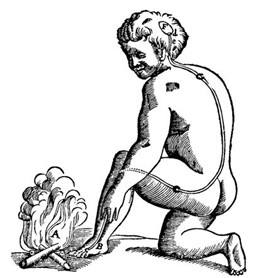
\includegraphics[width=4.16667in,height=\textheight,keepaspectratio]{images/DescartesWikipedia.jpg}

}

\caption{\label{fig-descartes}Descartes Schmerzmodell (1662)}

\end{figure}%

Heute denken wir, dass Schmerz zwar grundsätzlich von diesem Prinzip
herrührt, jedoch viel weiter geht. Wie wir Schmerz empfinden und ob wir
Schmerz empfinden, ist einerseits von biologischen Faktoren, aber auch
von psychischen und sozialen Faktoren abhängig. Wir können Schmerzen in
manchen Situationen gut ertragen oder sogar genießen und in anderen
Fällen die gleiche physische Quelle des Schmerzes als unerträglich
einstufen (für eine einfache, anwendbare Übersicht zu Schmerztheorie:
Butler and Moseley 2016; weiters Egger 2017; Mescouto et al. 2022).

Das BPS-Modell geht heute noch viel weiter. Auch anderer Bereiche sind
direkte oder indirekt von psychosozialen Faktoren beeinflusst. Du hast
dich bereits im Prozess der Anamnese und der Motivation mit psychischen
und sozialen Faktoren beschäftigt. Du hast dich und deine Klient*innen
gefragt, welche Personen sie in ihren Vorhaben unterstützen können, wie
sie mit Stress und Schlaf umgehen oder wie sie ihre Training in den
Alltag einbauen können.

Wenn wir Trainingspläne schreiben, über Motivation reden, Lifestyle
Coaching betreiben und Ziele besprechen, sollten wir immer an vier
Ebenen denken:\\
\textbf{Biologie}: Was wäre biologisch/physiologisch die richtige
Herangehensweise?

Z.B. ist „kcal in kcal out`` der wichtigste biologische Faktor um
abzunehmen.

\textbf{Psychologie:} Welche psychologischen Hindernisse oder Barrieren
bestehen für diesen Menschen?

z.B. ist vielleicht Intermittierendes Fasten eine psychologische Hilfe
um „kcal in kcal out`` zu optimieren (vergl. Aragon and Schoenfeld
2022).

\textbf{Soziologie}: Welche sozialen Faktoren spielen eine Rolle?

z.B. Kann mein Kunde mit „Dinner canceling`` nicht mehr am gemeinsamen
Familienabendessen teilnehmen.

\textbf{Umfeld:} Wie beeinflussen Klima, Infrastruktur, Wohnsituation,
Arbeitsweg unseren Entscheidungsprozess?

z.B. Gibt es nur fixe Mahlzeitengrößen in der Büro-Kantine; Heißer
Sommertag erschwert für viele Menschen die Nahrungsaufnahme zu Mittag.

\section{Klientenzentriertes Coaching
(CCC)}\label{klientenzentriertes-coaching-ccc}

CCC bedeutet, dass wir die Prozesse, die wir durchlaufen an die
Kund*innen anpassen. Das Gegenteil davon ist ein \textbf{Trainer*innen-
oder Traditionszentrierter Ansatz}. Diese beiden Modelle sind in
Aussagen wie: „Das haben wir immer so gemacht!{}``, „Ich trainiere auch
so``, „Sportler*in X trainiert auch so!{}``, „Das funktioniert bei allen
meinen anderen Kunden!{}``

Das Problem an diesen Ansätzen ist offensichtlich. Es geht nicht auf die
Individualität der Klient*innen ein. Jedoch schaffen es PCs so sich ihr
Weltbild intern aufrecht zu halten. Denn: Wenn es nicht klappt, ist die
Kundin zu „willensschwach, dumm, unmotiviert\ldots``. Wenn es jedoch
klappt, ist das wieder ein „Beweis`` für mein funktionierendes System.

Der CCC Ansatz basiert ursprünglich auf den Annahmen des Psychologen
Karl Rogers (Personenzentierte Psychotherapie). Er stellte sechs
Bedingungen für eine gelingenden Therapie auf, die sich auch heute noch
als entscheidend herausstellen. (Einige Zeit wurde sogar in
wissenschaftlichen Kreisen diskutiert, dass sie die einzigen wirkenden
Kräfte in der Psychotherapie sind (Cuijpers, Reijnders, and Huibers
2019).) Die vier für uns wichtigsten Grundannahmen, die Rogers auch
immer weiter ausgebaut hat sind (Egger 2017):

\begin{itemize}
\tightlist
\item
  \textbf{Bedingungslose positive Wertschätzung}
\end{itemize}

Dies bedeutet, dass Therapeut*innen die Klient*innen nicht bewerten,
sondern deren Erfahrungen anerkennen. Nur so ist es auch möglich die
drei Pfeiler des EBC (siehe weiter unten) voll anzunehmen.

\begin{itemize}
\tightlist
\item
  \textbf{Empathie / Einfühlungsvermögen und Gegenwärtigkeit}
\end{itemize}

Die Therapeut*innen fühlen sich in die Klient*innen ein, um die
Erfahrungswelt ihrer Gegenüber zu prüfen. Sie sind bei Ihnen anstatt bei
ihrer persönlichen Erfahrungswelt.

\begin{itemize}
\tightlist
\item
  \textbf{Kongruenz / Echtheit}
\end{itemize}

Die Therapeut*innen sind in ihrer Rolle mit ihrem Selbstbild kongruent.
Klient*innen sind dies oft nicht (laut Rogers sind sie das in der
Psychotherapie (!) nie). Die Therapeut*innen versuchen diese Echtheit
auch nicht zu überspielen, sondern zeigen sich ebenfalls als
verletzlicher Mensch. Die Klient*innen kommen mit einem Problem (sie
fühlen sich nicht fit oder nicht attraktiv\ldots). Sie sehen auch oft zu
anfangs nicht, dass die meist jungen, fitten Trainer*innen ebenfalls
ähnliche Herausforderungen haben. Echtheit schafft Gemeinsamkeit und
Zugehörigkeit.

Client Centered Care wurde später auch in der Pflegewissenschaft und
Medizin wieder neu aufgefasst.

Im Zentrum steht der humanistische Ansatz von Rogers. Der Mensch
(„Patient*in`` wird als Wort hier meist abgelehnt) soll selbstwirksam
(\textbf{empowered}) werden können und wird in alle
Entscheidungsprozesse miteinbezogen (\textbf{shared decision making}).
Die Aufgaben der Helfer*innen ist es, eine \textbf{partnerschaftliche,
respektvolle, transparente und auf Vertrauen aufgebaute Beziehung zu
ermögliche und zuzulassen} (Louw, Marcus, and Hugo 2017).

\section{Evidence Based Coaching (EBC)}\label{sec-EBM}

Evidence Based Medicine (EBM) wurde durch David Sackett ins Leben
gerufen. Es wurde zusammengefasst als ein System das auf drei Säulen
ruht:

\begin{itemize}
\tightlist
\item
  \textbf{Die wissenschaftliche Evidenz (Forschung, Studien\ldots)}
\item
  \textbf{Die Erfahrung der Klient*innen}
\item
  \textbf{Die Erfahrung der Helfenden}
\end{itemize}

Sackett wird nachgesagt, dass er meinte Fachbücher gehören verbrannt, da
sie veraltetes Fachwissen mit der Meinung der Autor*innen mischen. Die
Autor*innen sind aber nicht bei einer Therapie (oder Training) mit den
Klient*innen dabei, sondern die Therapeut*innen/Trainer*innen und die
Klient*innen.

Die drei Grundpfeiler der \textbf{EBC sind gleichermaßen wichtig!} Es
ist also nicht möglich nur auf Studien aufbauend ein Training zu
gestalten, da keiner eurer Klient*innen den Teilnehmer*innen in den
Studien entspricht und ihr als Trainer*innen andere Kompetenzen
mitbringt als das Forscherteam (zusätzlich zu Ausrüstung und
Infrastruktur). Es ist auch nicht möglich nur auf die eigenen
Erfahrungen zu hören, da die meistens gebiased sind, jede*r einzelne PC
mehr blinde Flecken hat als ungetrübtes Blickfeld.

\emph{„Evidence based medicine is not ``cookbook'' medicine. Because it
requires a bottom up approach that integrates the best external evidence
with individual clinical expertise and patients' choice, it cannot
result in slavish, cookbook approaches to individual patient care.''}
(Sackett et al. 1996, 72)

Sowohl in der Medizin als auch in Exercise Science ging der Trend in den
letzten Jahren mehr und mehr wieder in Richtung EBM Modell.

Durch die größer werdende Datenmenge, die wir von jeder Person bekommen
(durch Wearables und Körper-Maschinen Schnittstellen) erhoffen sich
viele jedoch wieder ein objektivieren und optimieren von
Gesundheitsinterventionen. Ein Push von Seiten der Biomedizin-Hardliner,
der, wenn nicht ganz unnötig, sicherlich verfrüht kommt. Noch sind wir
nicht so weit, dass wir Menschen nur als die Summe ihrer gemessenen
Biomarker betrachten können und Training beispielsweise an die Genetik
anpassen können. Leider sehen wir in der Fitnessbrache oft Scharlatane,
die versuchen über Zahlen und Messdaten Rückschlüsse auf ein „optimales
Trainingprogramm`` zu machen.

Dazu lässt sich nur im Stil von Tyler Durden antworten: „You are not
your f*cking Testosteron level!{}``

\section{Weitere Überlegungen}\label{weitere-uxfcberlegungen}

\subsection{Schuld}\label{schuld}

Der Fitnessbereich arbeitet häufig mit einer Strategie, die die Kirche
seit gut 2000 Jahren erfolgreich perfektioniert hat. Die Idee von Schuld
(z.B. am Gewicht und Gesundheit) ist stark in unsere Kultur und in unser
Denken integriert. Im Unterschied zur Religion sollten wir uns aber klar
sein, dass unser Ziel nicht ist, möglichst viele „Sünder`` möglichst
lange im System Kirche/Fitness-center zu halten, sondern sie von dieser
Idee der Fitness vielleicht sogar ein Stück zu befreien und anstelle von
Unzufriedenheit mit sich selbst, etwas anderes zu erleben, wenn sie in
den Spiegel schauen.

Wer die Schuldkarte spielt schafft lediglich Abhängigkeit und
Unzufriedenheit. Für die Coaches, die die Schuldkarte spielen, ist es
jedoch doppelt angenehm: wenn Klient*innen versagen ist es deren Schuld,
wenn sie jedoch ihr Ziel erreichen, ist es mein Verdienst.

Frag dich mal selbst ernsthaft: Ist es jemandes Schuld\ldots{}

\begin{itemize}
\tightlist
\item
  \ldots{} nicht fit zu sein?
\item
  \ldots{} Nicht intelligent zu sein?
\item
  \ldots{} zu rauchen?
\item
  \ldots{} Übergewichtig zu sein?
\end{itemize}

Frage dich ernsthaft und geh richtig in die Tiefe. Wo startet dessen
Schuld? Wo ist der Punkt im Leben der Person an der sie selbst schuldig
ist?

\subsection{Sünden}\label{suxfcnden}

Was fällt dir ein, wenn du an Sünde denkst - Sex oder Essen?

Viele eurer Kund*innen haben gelernt, dass es Sünden (gerade beim Essen)
gibt. Man kann natürlich Buße tun, indem wir uns bewegen und alles
ungeschehen machen. Manchmal ist Gemüse auch der Ausgleich zur Sünde.
Wir werden von den Sünden losgesagt.

Die eigentliche Idee hinter der Buße war jedoch die Vergebung. Jedoch
bleibt diese im modernen Sinn außen vor. Niemand verzeiht sich selbst
für die Schokolade. Solange das jedoch nicht passiert und die Menschen
nicht auch in Frieden und Akzeptanz mit ihrem Hang zu Schokolade sein
können, dreht sich die Spirale weiter um Selbsthass und „ausbrennen der
Sünde``.

Wichtig ist natürlich, dass Buße tun (= Gemüse oder Sport) niemals Spaß
machen darf! Somit darf ich ja Sport auch nicht genießen. Es ist
schließlich meine Buße. So absurd es scheint, ist es doch Teil unseres
Gedankengutes.

Solange Klient*innen nicht erkennen welche Bedürfnisse sie sich durch
die Handlung, die sie als Sünde abstempeln erfüllen und damit diese auch
wohlwollend annehmen, solange können sie auch das gesunde Essen/die
Bewegung nur als Buße ansehen. Uns ist natürlich auch von einer
biologischen Sichtweise klar, dass schlechtes Verhalten nicht mit gutem
Verhalten wirklich auszugleichen ist. Wer die Kalorien an Keksen beim
Laufen ausgleichen versucht sieht ja nur einen Teil der Gleichung. Sport
ist mehr als nur Kalorien und Kekse sind ebenfalls mehr als Kalorien.

\begin{figure}

\centering{


\includegraphics[width=4.16667in,height=\textheight,keepaspectratio]{images/devildonuts.png}

}

\caption{\label{fig-Simpson}Simpsons}

\end{figure}%

\subsection{Mental Toughness and Grit}\label{mental-toughness-and-grit}

Der typische Coach-Hardass Ansatz von \textbf{Grit} (=
conscientiousness) besagt, dass wir einfach hart zu uns sein müssen.

„Just do it!{}`` (schlag mal nach woher Nike diesen Spruch hat)

„Zähne zusammenbeißen und durch!{}``

„Keine Müdigkeit vortäuschen!{}``

„Fake it till you make it!''

``Geist über Körper!{}``

Es geht zusammengefasst darum, die eigenen Gefühle abzustellen oder sie
zumindest nicht zu zeigen. Es hat sich jedoch herausgestellt, dass
dieser Ansatz mit einigen Problemen einher geht. Die Motivation steigt
schnell, fällt jedoch auch wieder rapide ab. Wenn Kund*innen diese Art
des Denkens länger durchhalten, dann nur auf Kosten anderer
Lebensbereiche, denn sie erfordert viel Willenskraft und Anstrengung.
Die Alternative ist es, Gefühle zu erkennen und zu benennen. Sie sind
unserer wichtigsten Fluginstrumente, die aber auch trainiert werden
müssen. Ja, Kund*innen haben Angst zu versagen, sie verspüren Scham in
der Umkleide oder Ekel vor sich selbst oder vor vielbenutzten
Hantelbänken. Aber auch wir als Trainer*innen haben Angst - zum Beispiel
vor unserer eigenen Ohnmacht beim Umgang mit den Gefühlen der
Trainierenden.

Grit und Mentale Toughness heißt nicht, keine Gefühle zeigen, sondern
diese klar zu erkennen (nicht so leicht), zu benennen und als eine
Einschätzung der Situation mitzunehmen. Als PCs sind wir nicht
therapeutisch ausgebildet. Wir können jedoch (wie im Sport, Ernährung
und Regeneration) mit gutem Beispiel voran gehen und unserer eigenen
Gefühle klar ansprechen.

Verlassen wir uns auf Just-do it Mentalität holen wir außerdem nur die
Kund*innen ab, die es sowieso schaffen würden ihre Ziele in der Fitness
zu erreichen. Ihnen ist dieser Lebensbereich besonders wichtig und sie
haben die Zeit und Ressourcen den Zielen nachzugehen. Genau aus diesem
Grund scheint es auch so, dass Coach-Hardass auch mehr Erfolg hat als
Coach-Mitgefühl. Ersterer hat auch Klient*innen die zu dieser
Philosophie einen Zugang finden. Die anderen springen ab oder werden
grundsätzlich nicht angesprochen.

Buchempfehlung dazu, relevant für den Sportsektor:
\url{http://www.stevemagness.com/do-hard-things/}

\subsection{Probleme kreieren um sie zu
lösen}\label{probleme-kreieren-um-sie-zu-luxf6sen}

Eine häufige Strategie von Trainer*innen und Therapeut*innen ist es,
Probleme aktiv zu suchen, um sie dann zu lösen. Das beeindruckendste
Beispiel dafür sind die \textbf{Memory Wars} der letzten 20 -- 30 Jahre.
Psychotherapeut*innen und Psycholog*innen gelang es mehrmals „verborgene
Erinnerungen`` an z.B. Vergewaltigungen in Personen aufzudecken. Das
Problem dabei: einige der Personen hatten nie eine Vergewaltigung,
konnten aber durch suggestive Techniken und Hypnotherapie dazu gebracht
werden, sich leibhaft an eine solche zu erinnern (Ost et al. 2013). Dies
geschah natürlich nie aus Böswilligkeit der Therapeut*innen, sondern aus
der Überzeugung heraus, dass da doch ein Problem sein muss!

\emph{„Sie reagieren so defensiv auf diesen Typus von Männern -- haben
sie jemanden in der Familie der so ähnlich ist? Welche
Kindheitserinnerungen haben sie an diesen Onkel? Und da ist wirklich nie
etwas besonderes vorgefallen? Bei Ihrem Verhältnis zu Männern, muss da
irgendetwas dahinter stecken\ldots``}

Nun, das Gleiche passiert in der physischen Praxis zum Beispiel mit
Haltung. Es wird das Problem der „schlechten Haltung`` kreiert, das dann
durch die Expert*innen wieder verbessert werden kann.

\emph{„Sie haben eine so schlechte Haltung! Haben Sie Rückenschmerzen?
Nein -- Na das kommt noch, wenn wir nicht gleich was machen!{}``}

Ein anderes Beispiel ist Chiropraktik
(\url{https://youtu.be/t2yBlozgWuc}). Hier wird (konträr zu jeder
wissenschaftlichen Forschung ein alternatives Modell erstellt. Dinge,
die die Wissenschaft nicht sieht und nur die eingeweihten
Chiropraktiker*innen (mit ihrem geheimen Wissen) erfühlen können\ldots{}

Wir sind alle gefährdet in diese Falle zu tappen und unseren
Klient*innen mehr Probleme anzudichten, als gut ist. Wir müssen uns ja
auch verkaufen und uns selbst unsere Profession, das jahrelange Studium
und die hohen Preise rechtfertigen.

\subsection{Was sie wollen und was sie
brauchen}\label{was-sie-wollen-und-was-sie-brauchen}

Wir müssen uns immer fragen, ob wir den Kund*innen das geben, sollen was
sie brauchen (unser PC Blickpunkt) oder was sie möchten (ihr
Blickpunkt).

Einerseits sind wir Dienstleister*innen und sollten uns auch so
verhalten (die Kund*innen möchten etwas und wir liefern), andererseits
können die Kund*innen oft nicht richtig einschätzen was sie brauchen.
(„Ich brauche mehr Bauchmuskelübungen um mein Bauchfett zu verlieren.``)

Es kommt hinzu, dass wir in gewisser Weise von unseren Kund*innen
abhängig sind und Trainer*innen befürchten, dass Kund*innen abspringen,
wenn wir nicht das machen, was sie möchten. Gleichzeitig sollten Sie auf
lange Sicht ihre Ziele erreichen und dabei keine gesundheitlichen
Risiken eingehen.

Denke an CCC. Es geht nicht darum, dass Klient*innen die Entscheidungen
treffen was wir machen, aber auch wir treffen sie nicht alleine. Es geht
um einen Austausch und \textbf{Shared Decision Making}. Dies gelingt nur
bei klarer Kommunikation auf Augenhöhe und gut definierter Berufsethik
(siehe @ref(Ethik))

\subsection{Kundenbindung}\label{kundenbindung}

Viele PCs denken an Kundenbindung. Sie möchten Klient*innen so lange wie
möglich behalten und sind sogar stolz auf Klient*innen die schon
jahrelang mit ihnen trainieren. Dies ist nicht an sich schlecht.

Ab einem bestimmten Punkt sollten wir uns fragen wie viel wir den
Kund*innen noch beibringen können und inwieweit die professionelle
Beziehung mit unseren Kund*innen noch beibehalten werden kann. Auch aus
wirtschaftlicher Sicht ist es nicht nachhaltig, auf Kundenbindung zu
setzen. Auch die PCs binden sich schließlich an die Klient*innen. Fallen
langjährige Kund*innen weg, kommt es schnell zu einer existentiellen
Krise. Auf der anderen Seite könnte es eine Strategie sein Klient*innen
immer schnellst möglich los zu werden. Wenn wir versuchen Kund*innen
möglichst alles wichtige beizubringen, so dass sie selbstwirksam
trainieren können, haben wir die Chance neue Klient*innen anzunehmen.
Jede zufriedene Kundin, der wir eigenständiges Training beibringen, ist
eine potentielle Multiplikatorin.

\subsection{Marketing mit
Testimonials}\label{marketing-mit-testimonials}

Wie entstehen Testimonials?

Selbst die besten Trainer*innen werden es nie schaffen, dass alle ihre
Kund*innen ihre Ziele erreichen. Aber auch die schlechtesten Coaches
haben vielleicht mal einen Glücksfall und eine wirklich gute Responderin
als Klientin oder eine Person, die gerade an einem Wendepunkt ihres
Lebens ist, ihre Ernährung von einem Tag auf den anderen umstellt und
bereit ist alles für ihre Gesundheit zu tun. Sie holt sich sogar einen
Personal Coach\ldots{} Nun, diese Person wird ein Testimonial. Die
hundert anderen werden es nicht.

Coach Hard-ass hat natürlich mehr Testimonials, da er/sie auch mehr
hardass Klient*innen anzieht.

\section{Literatur}\label{literatur-7}

\bookmarksetup{startatroot}

\chapter{Methoden des Coachings}\label{methoden-des-coachings}

\section{Aufbau von Einheiten}\label{aufbau-von-einheiten}

Die meisten Trainer*innen bieten Trainings zwischen 30 und 90min an. In
dieser Zeit sollen viele Bereiche abgedeckt werden:

\begin{itemize}
\tightlist
\item
  Begrüßung
\item
  kurzes einleitendes Gespräch

  \begin{itemize}
  \tightlist
  \item
    Smalltalk
  \item
    Fragen nach heutigem Empfinden
  \end{itemize}
\item
  Rückgriff auf Coaching Elemente seit letzter Einheit

  \begin{itemize}
  \tightlist
  \item
    Besprechung von eigenem Training
  \item
    Besprechen von Lifestyle Coaching (Ernährung,
    Stressmanagement\ldots)
  \end{itemize}
\item
  Mögliche Fortschrittsüberprüfungen
\item
  Absprechen der heutigen Einheit
\item
  Warm-up
\item
  Training
\item
  Cool-down
\item
  Besprechung der Übungselemente bis nächste Einheit
\item
  Terminvereinbarung
\end{itemize}

Es ist nicht immer einfach alles in 60min zu packen. Überlege dir gut,
welche Elemente der Einheit du für die jeweiligen Coachees auch
auslagern kannst. Können sie sich vor der Einheit eigenständig
Aufwärmen? Nein -- nun, dann ist es vielleicht dein persönliches Ziel,
dass sie das erlernen. Möchtest du Terminvereinbarungen außerhalb der
Trainingszeit lösen? Das ist großartig! Überlege dir nur ein gutes
System. Wenn du einmal 20 Kunden hast, ist es kein Spaß mehr über
Whatsapp flexibel Termine auszumachen.

Darüber hinaus haben auch Kund*innen gewisse Vorstellungen. Viele
möchten (bewusst oder unbewusst) mit einem gewissen Gefühl aus der
Einheit gehen. Das Training soll sie entweder mit Energie für den
Arbeitstag füllen (v.a. morgens, mittags), sie möchten sich am Ende
entspannt fühlen (v.a. am Abend oder am Wochenende) oder sie möchten das
Gefühl haben, dass sie alles gegeben und viel geleistet haben (sowieso
immer ).

\subsection{Wahrnehmung von subjektiver
Intensität}\label{wahrnehmung-von-subjektiver-intensituxe4t}

Eine wichtige Strategie, damit du und deine Klient*innen zufrieden aus
der Einheit kommen, ist die \textbf{Peak-End Regel} (Kahneman 2012).
Menschen erinnern sich am meisten an den Höhepunkt und an das Ende eines
Urlaubs, eines Lebensabschnittes, einer medizinischen Untersuchung und
eines Trainings. Kund*innen, denen es wichtig ist, dass sie sich sehr
verausgaben, reicht oft ein kurzer Block von 5-10 Minuten in den letzten
15 Minuten der Einheit. Unter anderem daher (aber im Fall des Trainings
sicher auch aus physiologischen Gründen), fühlt sich ein Training mit
einem kurzen Block von 10-15 hoch intensiven Elementen härter und
„effektiver'' an, als ein Training, das 50min bei 70\% Intensität liegt.
Nutze diese Regel, um das Training so anzupassen, dass es den
Erwartungen deiner Klient*innen entspricht.

Auf der anderen Seite steht das Heranführen an die geforderte
Trainingsintensität. Dies kennst du vielleicht aus deinem eigenen
Training. An manchen Tagen fühlt man sich nicht bereit für ein
intensives Training. Nach einem guten Warm-up und ein paar leichteren
Übungen kommt man jedoch manchmal doch noch in Schwung und übertrifft
sogar die eigenen Erwartungen. Diesem Effekt solltest du dir bewusst
sein, wenn Klient*innen dir erklären, dass heute sie „heute sehr müde
sind und Nichts gehen wird''. Gib ihnen Zeit, schreib die Einheit nicht
gleich ab. Vielleicht entwickelt sich eine eigene Dynamik und ihr könnt
zumindest einen kurzen Teil der Einheit im entsprechenden
Intensitätsbereich verbringen. Wenn dir das gelingt, ist es wichtig die
Klient*innen im Anschluss darauf aufmerksam zu machen. Frag sie, wie
sich das Energielevel während der Einheit verändert hat und was sie über
diesen geänderten Zustand denken. Halte ihre Einschätzung dabei
realistisch. Manchmal gelingt es den Organismus anzukurbeln. An anderen
Tagen ist es einfach besser es ruhig anzugehen. Mit der Zeit können sie
lernen ein Gefühl für den Unterschied zu bekommen. Du kannst ihnen
helfen indem du ihnen auch objektive Maße (Herzfrequenz,
Hantelgeschwindigkeit, Sprunghöhe, Griffkraft, HRV, RPE, \ldots{} oder
andere Parameter die Autoregulation ermöglichen) zu Verfügung stellst,
mit denen Sie ihre innere Wahrnehmung schulen können.

\emph{Hier erscheint in Kürze: ``Subjektive Wahrnehmung''}

\section{Abgleichen der Sichtweisen}\label{abgleichen-der-sichtweisen}

Um die Ansprüche meiner Klient*innen mit meinen Sichtweisen
abzugleichen, müssen wir sie kennen und besprechen! Die Frage nach der
\textbf{Erwartung} der Kund*innen an die Einheit ist dafür wichtig. Das
beutet jedoch nicht, dass wir diesen Erwartungen genau entsprechen
müssen. Wir sollten jedoch ansprechen können, wenn wir sie nicht
erfüllen wollen/können. Wenn Kund*innen glauben Training sei nur
„effektiv'', wenn sie sich total verausgabt haben und erschöpft sind,
wir aber der Meinung sind, dass kontinuierliches Training auf 80\%
langfristig mehr bringt, muss diese Diskrepanz besprochen werden. In den
meisten dieser Gespräche wirst du als Expert*in für Training und Fitness
sicher häufig das Gefühl haben, dass du natürlich die Wahrheit kennst
und recht hast. Es wird dir jedoch nicht immer gelingen Klient*innen von
ihren Überzeugungen mit guten Argumenten umzustimmen. Wie du mit diesen
Diskrepanzen umgehst, ist eine schwierige Frage, die du nicht auf die
leichte Schulter nehmen solltest.

Viele Berufsanfänger*innen (aber auch erfahrenere Coaches) halten es für
wichtig den Kund*innen das zu geben, was sie wollen. Gleichzeitig
verstärkst du dadurch falsche Annahmen bei deinen Kund*innen. Du wirst
außerdem deine Kompetenz interminieren und gleichwohl deinen eigenen
Ansprüchen nicht entsprechen können -- ein Teufelskreis aus dem du nur
schwer wieder heraus kommst.

Die konträre Herangehensweise ist es, von den eigenen Systemen nicht
abzuweichen und darauf zu beharren, dass alle deine Kund*innen dieses
Programm durchlaufen und ja schließlich Erfolg haben. Auch diese Ansicht
ist eine Sackgasse, aus der du nicht so schnell herauskommst. Du
verzichtest hiermit auf individuelle Ansprüche der Kund*innen (das
Herzstück von PT) und verwehrst dir die Möglichkeit dazuzulernen.

\textbf{Deine Aufgabe:} Besprich mit deinen Klient*innen ihre
Erwartungen an die Einheiten. Dann besprich mit ihnen ehrlich und
wertschätzend, was deine Meinung dazu ist. Überlege dann gemeinsam mit
ihnen, wie ihr hier einen gemeinsamen Weg finden könnt. Vielleicht
kannst du deine Kund*innen auch einen oder zwei Tage nach einem Training
kontaktieren und sie rückwirkend fragen, wie es ihnen mit dem Training
ging. Manchmal (meistens) passen das \emph{Erlebende Ich} und
\emph{Erinnernde Ich} auch nicht ganz zusammen. Besprich dann am Anfang
der nächsten Einheit auch das mit ihnen und frag sie, wie sie das
wahrnehmen und was eine gute Lösung sein könnte.\footnote{Du solltest
  immer die Klient*innen nach ihren Lösungen fragen. Halte aber
  mindestens eine Lösung, die von dir kommt, bereit. Schließlich (so das
  Argument der Klient*innen) wirst du ja für die Lösungen bezahlt.}

\textbf{Persönlicher Zwischenreport}

Arbeitet man mit Kund*innen langfristiger zusammen, so verlieren beide
nach einer gewissen Zeit manchmal den Fokus oder es schleifen sich
Muster ein, die für keinen der beiden Parteien zielführend
sind\footnote{Ein bisschen wie das Ehepaar und die Frühstückssemmeln bei
  Paul Watzlawick}. Gleiche Sichtweisen auch mit langfristigen Kunden
explizit ab. Man kann sich leicht täuschen oder aneinander vorbeireden.

Hierzu kann man zum Beispiel einen kurzen (!) Fragebogen vorbereiten,
den man den Klient*innen mit nach Hause gibt oder online zusendet.
Fragen zum vergangenen Trainingsprozess, ihre Einschätzung zur eigenen
Gesundheit und Fitness, Veränderungen, die sie durch das Training erlebt
haben, Erwartungen für zukünftige Einheiten, usw., können zum Beispiel
über Skalen oder offene Textfelder abgefragt werden. Als Nebeneffekt
stellt sich durch die Übung bei den Klient*innen oft eine Dankbarkeit
und Zufriedenheit mit ihren Veränderungen und ihrem Training ein.

Nutze den persönlichen Zwischenreport in der nächsten Einheit als
Einleitung für ein kurzes Gespräch über zukünftige Einheiten.

Ich persönlich nutze diesen Zwischenreport so, dass auch ich den
gleichen Fragebogen für die Kund*innen aus Trainer*innen-Sicht ausfülle.
Diese beiden Versionen können wir abgleichen und daraus unserer Schlüsse
ziehen.

\bookmarksetup{startatroot}

\chapter{Ausgewählte Methoden im
Coaching}\label{ausgewuxe4hlte-methoden-im-coaching}

Im Folgenden findest du ein paar Ideen, die du im Coaching anwenden
kannst. Geh mit der Intention in die Einheit, eine dieser Methoden
auszuprobieren und beobachte den Effekt bis zur nächsten Einheit.
Achtung: Keines davon sind die ultimativen Lösungen die immer und für
alle Kund*innen (und Trainer*innen) funktionieren. Probiere ein bisschen
herum und \emph{„Reject what is useless and add what is specifically
yours''} -- Bruce Lee

\section{Zeige es mir}\label{zeige-es-mir}

Viele Klient*innen haben hohe Ansprüche an sich selbst und übernehmen
sich häufig in ihren Vorhaben („5x die Woche 60min Laufen schaff
ich.''). Mit deiner Hilfe sollten sie realistische Ziele setzen, die sie
auch bewältigen können. Manchmal wird behauptet man soll diese Ziele so
klein wie möglich halten um sie dann zu erreichen (Clear, 2018). Dies
funktioniert aber nur, wenn die Klient*innen diesen Ansatz auch
akzeptieren können. Mehrmals habe ich mit diesem Ansatz die Erfahrung
gemacht, dass die Klient*in den Erfolg, den sie dabei erzielt haben
nicht annehmen konnten. Der „Success breeds success'' Ansatz
funktioniert jedoch nur, wenn die Person den Erfolg auch als einen
solchen verbuchen kann. Ist die Aufgabe zu einfach wird sie ihn als
selbstverständlich abtun. Die Attribution von Erfolg oder Misserfolg
einer Handlung ist immer von mehreren Faktoren abhängig. Ein gewisser
Schwierkeigkeitsgrad und das Gefühl sich angestrengt zu haben sind dabei
jedoch entscheidend (Schunk and DiBenedetto 2021).

Eine Möglichkeit damit umzugehen ist es die Klient*in damit
herauszufordern. „Ok, du denkst, dass diese Strategie für dich richtige
ist. Wunderbar -- zeige es mir, dass du es schaffst. Ich denke es ist
eine Herausforderung, aber ich glaube, dass du es schaffen kannst.
Danach leiten wir den nächsten Schritt ein.

\subsection{Verbesserungen verstehen}\label{verbesserungen-verstehen}

Die Grundlagen einer neuen Fähigkeit zu erlernen -- sei es kochen,
malen, eine Sportart oder gute Gespräche zu führen sind meist recht
einfach. Nach ein paar Fehlversuchen scheint man sich regelrecht mit
jedem Versuch linear zu verbessern. Mit zunehmendem Expertentum wird es
jedoch schwerer und schwerer weitere Verbesserungen zu erzielen. So ist
es auch mit vielen Prozessen die deine Klient*innen betreffen. Nach
einer anfänglichen Phase des Erfolgs wird es zunehmend schwieriger
besser zu werden. Nach wenigen Einheiten ist es möglich eine Strecke von
5km durchzulaufen, aber die Zeit zu verbessern wird zunehmend schwerer.
Die ersten Kilogramm purzeln schnell von der Waage, aber ein Six-pack
ist nicht von heute auf morgen erreichbar. Während dieser Umstand von
außen betrachtet einleuchtend erscheint, führt er aus der persönlichen
Perspektive zu Problemen. Der Umstand, dass der Fortschritt immer
langsamer werden kann und es auch Plateaus oder Regressive Momente geben
kann sollte früh genug kommuniziert werden. Auch hier ist die richtige
Kommunikation das A und O. Nachdem der erste Erfolg verbucht wurde, gilt
es erst mal zu feiern und die Klient*in auf die eigenen Anstrengungen
hinzuweisen, die es ihr erlaubt haben hier anzukommen. Plädiere beim
Übergang zum nächsten Ziel auf ihre neuen Fähigkeiten, die sie in diesem
Prozess erlernt hat. Nun ist es ihr möglich eine neue Herausforderung
anzugehen.

Nach einer Phase der Zielerreichung sollten wir mit unseren Klient*innen
außerdem bewusst über den Prozess der Plateausisierung sprechen. Dieses
Plateau ist jedoch nicht nur ein Hindernis am Weg zu weiterem Erfolg
sondern kann als weiteres Lerninstrument genutzt werden. Das Plateau,
das sich womöglich von selbst einstellt (z.B. nach den ersten 5kg
Gewichtsreduktion) kann es als klares Ziel formuliert werden jetzt
diesen Erfolg zu stabilisieren. Diese Phase kann auch genutzt werden um
neue Energie zu tanken da es meist leichter ist erreichte Erfolge zu
halten als neue oben drauf zu packen.

{\emph{Hier erscheint in Kürze: ``Schwierigkeit von Aufbaben'',
``Fertiggerichte und Eigenkontrolle'', ``Erinnerungen'', ``Wiederholen
ohne wiederholen'' und ``Magische Frage''}}

\section{Literatur}\label{literatur-8}

\bookmarksetup{startatroot}

\chapter{Motorisches Lernen und Lehren}\label{sec-motorlearning}

Einer der offensichtlicheren Aufgaben im PT ist es, Menschen Bewegungen
und Übungen beizubringen. Motorisches Lernen ist ein großes Kapitel. Wie
in allen Bereichen, die wir bisher bearbeitet haben, geht es als PT*in
nicht darum jedes Detail zu wissen, sondern die Basis anwenden zu
können. Die Theorien sollten wir soweit verstehen, dass wir sie im Fall
der Fälle auch verständlich erklären und anwenden können.

Ziel des Kapitels ist es, dass du\ldots{}

\begin{itemize}
\tightlist
\item
  \ldots{} den Unterschied zwischen dem Lernen von Bewegungsverhalten
  und dem Lernen von Übungen verstehst und dadurch zielgerichtet die
  richtigen Methoden des Lehrens einsetzen kannst.
\item
  \ldots{} den Unterschied zwischen akuter Leistungsverbesserung und
  Lernen kennst.
\item
  \ldots{} Vor- und Nachteile von Organisationsformen (geblocktes üben,
  serielles üben, randomisiertes üben) aus Sicht des motorischen Lernens
  richtig einsetzen kannst.
\item
  \ldots{} verschiedene Methoden der Aufmerksamkeitsrichtung für
  Klient*innen zielgerichtet einsetzen kannst.
\item
  \ldots{} verschiedene Feedbackmöglichkeiten einsetzen kannst -- wann,
  wie viel, welche Art von Feedback\ldots{}
\end{itemize}

\section{Bewegungsverhalten oder Übungen
erlernen}\label{bewegungsverhalten-oder-uxfcbungen-erlernen}

Ich möchte als erstes auf den Unterschied zwischen \textbf{Lernen von
Bewegungsverhalten (Kategorie 1)} und \textbf{Lernen von Übungen
(Kategorie 2)} hinweisen. Diese dichotome Einteilung ist rein zur
Veranschaulichung gedacht und tritt in reiner Form nur selten auf. Die
Einteilung soll uns helfen, dass wir uns bewusst für einen Lehrstil
entscheiden können und dabei Vor- und Nachteile der Ansätze nicht aus
den Augen verlieren. Die Unterscheidung wird auch so nicht in der
Fachliteratur getroffen, sondern bezieht sich auf meine Beobachtung,
dass eine solche (oder ähnliche Unterscheidung) als implizite Annahme
den meisten Lehrkonzepten zugrunde liegt.

Unter dem \textbf{Lernen von} \textbf{Bewegungsverhalten} sollen hier
sportliche Fertigkeiten (Skills) oder das Wiedererlernen von
Alltagsbewegungen in der Rehabilitation verstanden werden. Unter dem
\textbf{Lernen von} \textbf{Übungen} werden hier „Fitness-'' oder
Trainingsübungen verstanden, die eine spezielle Form aufweisen sollen,
damit sie effektiv sind. Der Übergang zwischen diesen beiden Bereichen
ist nicht immer klar und es gibt Überschneidungspunkte. Auf den ersten
Blick scheint es so, als würden sich diese beiden Kategorien nur durch
die Vertiefungsstufe des Lernens unterscheiden (z.B.
\href{https://us.humankinetics.com/blogs/excerpt/understanding-motor-learning-stages-improves-skill-instruction}{Konzepte
nach Fitss oder Gentile}). Diese Unterteilung ist jedoch meiner Meinung
nach nicht ausreichend.

Es gibt auch populäre Ansätze, die keinen Unterschied zwischen diesen
Feldern sehen und zumeist unter die Konzepte von „Functional Training''
(vor allem verbreitet seit Verstegen and Williams 2011) oder „Contextual
Training'' (Bosch 2018) fallen können. Wobei es keine Einigkeit zwischen
den verschiednenen Ansätzen gibt. Der verbreitete Begriff des
\emph{Functional trainings} bleibt ohnehin nicht kritiklos (Ide et al.
2021)\footnote{Ide et al. (2021) kommen zu dem Schluss, dass die Beste
  Definition für \emph{Functional Training} von Fleck und Kraemer
  erstellt wurde. Sie nennen \emph{Functional Training} ``{[}\ldots{]}
  training that is meant to increase performance in some type of
  functional task {[}\ldots{]}'' (Fleck and Kraemer 2014 S. 247). Dies
  kann Aktivitäten des täglichen Lebens oder Sportarten beinhalten.}.
Beide fallen aber ebenfalls in den Bereich des sportspezifischen
Trainings. Auch in der Physiotherapie wird traditionellerweise häufig
ein „funktioneller'' Übungsansatz vorgeschlagen, der keine Grenzen
zwischen den Übungen und den Alltagsfunktionen sieht (z.B. Adler,
Beckers, and Buck 2007). Alle diese Konzepte gehen davon aus, dass es
einen starken Transfer vom Geübten zum Alltag oder zur sportlichen
Leistung gibt. So soll zum Beispiel eine Übung einen Bewegungsablauf im
Sport simulieren.

Eine gegensätzliche Meinung wird ebenfalls propagiert und behauptet,
dass das S\&C Training lediglich Energiesysteme und Strukturen
vorbereiten kann, dies jedoch unabhängig von der Sportart ist. Bekannte,
sehr unterschiedliche Vertreter dafür sind zum Beispiel Poliquin oder
Boyle. Wobei letzterer trotzdem von functional training spricht. Der
Sport muss also eigenständig betrachtet und trainiert werden. Alle diese
Konzepte sind natürlich berechtigt und bieten Vorteile, zeigen sich aber
nicht generell überlegen und weisen einige theoretische und praktische
Schwierigkeiten auf, die auch im Fitness- und Gesundheitssport Relevanz
finden.

\begin{longtable}[]{@{}
  >{\raggedright\arraybackslash}p{(\linewidth - 4\tabcolsep) * \real{0.2000}}
  >{\raggedright\arraybackslash}p{(\linewidth - 4\tabcolsep) * \real{0.4000}}
  >{\raggedright\arraybackslash}p{(\linewidth - 4\tabcolsep) * \real{0.4000}}@{}}
\caption{Bewegungsverhalten vs.~Übungen
erlernen}\label{tbl-MotL1}\tabularnewline
\toprule\noalign{}
\begin{minipage}[b]{\linewidth}\raggedright
\end{minipage} & \begin{minipage}[b]{\linewidth}\raggedright
\textbf{Kategorie 1} \textbf{Lernen von Bewegungsverhalten}
\end{minipage} & \begin{minipage}[b]{\linewidth}\raggedright
\textbf{Kategorie 2} \textbf{Lernen von Übungen}
\end{minipage} \\
\midrule\noalign{}
\endfirsthead
\toprule\noalign{}
\begin{minipage}[b]{\linewidth}\raggedright
\end{minipage} & \begin{minipage}[b]{\linewidth}\raggedright
\textbf{Kategorie 1} \textbf{Lernen von Bewegungsverhalten}
\end{minipage} & \begin{minipage}[b]{\linewidth}\raggedright
\textbf{Kategorie 2} \textbf{Lernen von Übungen}
\end{minipage} \\
\midrule\noalign{}
\endhead
\bottomrule\noalign{}
\endlastfoot
\textbf{Ziel} & Bewegungen so erlernen, dass sie möglichst unterbewusst
und automatisiert ablaufen können (Gehen, Laufen, Frontkick,
Carving-Schwung\ldots) & Übungen so ausführen, dass sie einen hohen
Anspruch auf die Zielstruktur oder das Zielsystem haben (aerobes,
anaerobes System, spezielle Muskeln, Faszien, Propriozeption\ldots) \\
\textbf{Energieumsatz} & Minimalisieren: Ziel ist es, die Bewegung
einfach und ohne übermäßigen Aufwand auszuführen & Optimierung: Das zu
trainierende System sollte (hoch) belastet werden, andere Systeme sollen
geschont werden, um sie nicht zu überlasten. \\
\textbf{Äußerer Fokus} & Zumeist ein äußerlicher Effekt in der Umwelt
oder eine körperliche Leistung (maximal weit, maximal schwer, hohe
Präzision, \ldots) & Zumeist ein Fokus auf Belastungs-Metrik, die nicht
unbedingt maximal sein muss (Volumen, Belastungsdichte, Herzfrequenz,
\ldots) \\
\textbf{Innerer Fokus} & Mit Bildern verbunden „\emph{Fly like a
butterfly and sting like a bee!}'' & Auf „richtige Ausführung'' nach
vorgegebenen Standards oder nach körperlicher Wahrnehmung (maximale
Muskelspannung, subjektive Belastung) \\
\textbf{Vorschlag für dazu passende Lehrkozepte} & Externale
Zielsetzung, Impliziter Lehrstil, (Differenzielles Lernen),
Kontextualisieren der Aufgaben (\emph{Adaptation}), Sequentielles oder
randomisiertes Üben & Internale Zielsetzung, Expliziter Lehrstil,
Maximale Sicherheit, keine Kontextualisierung notwendig, Blockweise oder
serielle Organisation je nach Zielsystem \\
\end{longtable}

In Table~\ref{tbl-MotL1} werden die beiden Lernziele unterschieden und
der daraus propagierte Lehransatz zusammengefasst. Die Kategorie 1
beschäftigt sich mit Bewegungen, die automatisiert werden sollen, häufig
kontextabhängig eingesetzt werden müssen (ein Pass muss immer etwas
anders aussehen, je nach Spielsituation; ein Schritt muss dem Untergrund
und der Ganggeschwindigkeit angepasst werden\ldots) und die Bewegung
sollte am Ende leichtfallen und möglichst wenig Energie benötigen. Im
Training von Fitnessübungen soll die Belastung einer bestimmten Struktur
(z.B. einzelne Muskeln) hoch ausfallen, damit es zu einem
Anpassungsprozess kommt. Dabei ist die Ökonomie der Bewegung oft
gewünscht sehr gering. Jedoch sollte die Übung so erstellt werden, dass
unnötige Belastungen vermieden werden.

Im Sinne dieses Unterschieds kann das folgende Video als schlechter
Bizepscurl aus Sicht Kategorie 2 oder als sehr guter Curl in Kategorie 1
betrachtet werden.

\url{https://youtu.be/Sqs1SRpcpeQ}

Diese Gegenüberstellung sollte dem Lehransatz entsprechend
berücksichtigt werden. Die meiste Grundlagenliteratur zum motorischen
Lernen beschäftigt sich mit Kategorie 1 (Magill and Anderson 2021;
Schmidt et al. 2019). Daraus ergeben sich auch viele Vorschläge für
Personal Trainer*innen und \emph{Strength and Conditioning (S\&C)
Coaches} auf Basis der Erkenntnisse von Magill, Schmidt oder Wulf. Die
genau gegensätzliche Herangehensweise wird in Systemen propagiert, die
vom klassischen Bodybuilding („the pump'') oder in körperzentrierten
Bewegungsmethoden (Yoga, Feldenkrais\ldots) inspiriert sind. Also wer
hat recht? \url{https://youtu.be/-xZQ0YZ7ls4?t=19}

Natürlich keiner und alle. Aber um uns klar zu werden, welche Art des
Bewegungslehrens wir wann verwenden wollen, müssen wir ein paar
Grundlagen zu \textbf{Motor Control} \textbf{und Motor Learning}
wiederholen:

\section{Performance vs.~Learning}\label{performance-vs.-learning}

Eine wichtige und häufig übersehene Differenzierung ist jene zwischen
\textbf{Performance (P) Leistung} und \textbf{Learning (L) Lernen}
(Schmidt et al. 2019). P bezeichnet die Fähigkeit, die jetzt im Moment
vorliegt. Diese P kann sehr variabel sein und so gelingen Anfänger*innen
vielleicht 5 von 10 Basketball Freiwürfen. Eine halbe Stunde später
gelingen der gleichen Person 1 von 10 oder 9 von 10.

\begin{figure}

\centering{

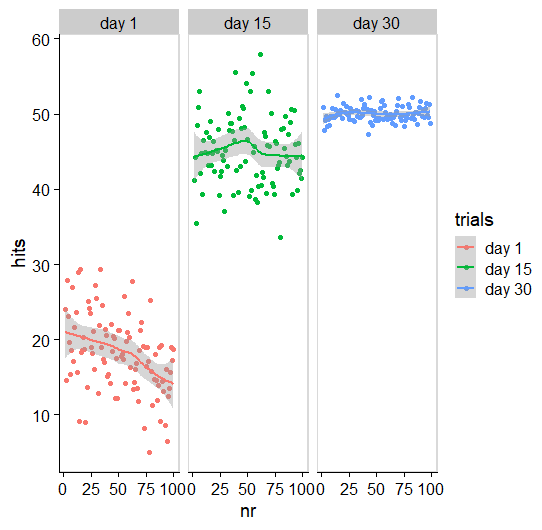
\includegraphics[width=4.16667in,height=\textheight,keepaspectratio]{images/MotL_sim1.png}

}

\caption{\label{fig-simA}Simulation Leistung vs.~Lernen 1}

\end{figure}%

Figure~\ref{fig-simA} zeigt ein simuliertes Beispiel, das dir den
Unterschied zwischen Lernen und Performance erklären soll. Hier macht
eine Person immer 100 Versuche einer Übung und bekommt dafür Punkte. Am
ersten Tag (rot) bekommt sie im Durchschnitt 20 Punkte (= P). Jede
Wiederholung sieht aber anders aus. In diesem Beispiel sieht es sogar so
aus, als würde sie am Ende des Tages schlechter sein als am Anfang (= P
sinkt)! Trotzdem, nach 15 Tagen üben (grün) ist die Person viel besser
geworden (= Lernen). Sie bekommt im Schnitt 45 Punkte (= P). Die
Wiederholungen sind alle noch immer sehr unterschiedlich. Nach weiteren
15 Tagen bekommt sie im Durchschnitt nur 5 Punkte mehr, jedoch ist ihre
Variabilität geringer geworden. Dies ist ein typisches Muster im
Lernprozess einer Person.

Veränderungen in der Performance sind ähnlich zu akuten Auswirkungen von
Ausdauer- oder Krafttraining - sie haben wenig damit zu tun, was
chronisch passiert. So macht ein einzelnes Ausdauertraining vielleicht
kurzzeitig müde und weniger leistungsfähig, mehrere machen jedoch
langfristig ausdauernder. \textbf{Lernen} \textbf{L} ist genau dieser
zweite Schritt und wird als ein langfristiger Prozess verstanden, der an
sich nicht beobachtbar ist (Schmidt et al. 2019). Bleiben wir beim
Beispiel aus dem S\&C so ist dir vielleicht bewusst, dass die aktuelle
Leistungsfähigkeit in einem Countermovement Jump (CMJ) recht leicht
manipuliert werden kann. Zum Beispiel kann das richtige Warm-up und ein
gut gesetzter PAPE Effekt deine Sprungleistung stark erhöhen (Seitz and
Haff 2016a). Du wirst aber nicht auf die Idee kommen, dass deine
Sportler*in nach einem guten Warm-up gelernt hat, jetzt dauerhaft höher
zu springen. Dir ist bewusst, dass das ein temporärer Zustand ist. (Eine
Gruppe aus Deutschland kommt in einem Review zu diesem speziellen Thema
zu dem Schluss, dass es möglicherweise auch zu langzeitigen
Verbesserungen kommt (Lesinski et al. 2014), konnten dieses Resultat
aber in einem eigenen RCT nicht bestätigen (Wallenta et al. 2016).

Auf eine ähnliche Weise sollte nicht angenommen werden, dass eine
Person, der ich jeden Schritt einer Übung genau zeige und daraufhin die
Übung am Ende der Einheit auch besser macht (P), dies auch
\textbf{gelernt (L)} hat! Sie hat \textbf{lediglich P erhöht}.

\begin{tcolorbox}[enhanced jigsaw, colback=white, toptitle=1mm, opacitybacktitle=0.6, title=\textcolor{quarto-callout-tip-color}{\faLightbulb}\hspace{0.5em}{Tip}, colframe=quarto-callout-tip-color-frame, colbacktitle=quarto-callout-tip-color!10!white, toprule=.15mm, rightrule=.15mm, bottomtitle=1mm, left=2mm, arc=.35mm, opacityback=0, titlerule=0mm, coltitle=black, breakable, leftrule=.75mm, bottomrule=.15mm]

\textbf{MERKE: Verbesserungen in der Leistung während der Einheit, hat
grundsätzlich nichts mit der dauerhaften Verbesserung der Leistung im
Sinn von Lernen zu tun!}

\end{tcolorbox}

Eine weitere Änderung des motorischen Verhaltens passiert durch
\textbf{Adaptionen} (Motor Adaptations). Hierunter verstehen wir zum
Beispiel \textbf{Kontext} \textbf{Änderungen} (Magill and Anderson
2021). Adaptionen sind feine Anpassungen in der Ausführung der Bewegung.
Selbst scheinbar sehr repetitive Bewegungen oder \textbf{Closed}
\textbf{Skills} sind immer leicht variabel in ihrer Ausführung. Eine
typische Adaption passiert beispielsweise, wenn eine geübte
Laufsportlerin schon lange nicht mehr (oder noch nie) auf einem Laufband
gelaufen ist. Die ersten fünf Minuten sehen seltsam aus und fühlen sich
möglicherweise für sie auch seltsam an. Die Variabilität der Schritte
ist dabei anfangs hoch, dann nimmt die Variabilität ab und die Läuferin
hat eine Adaption ihres Laufmusters gefunden. Steigt sie am nächsten Tag
auf das Laufband, dauert der Prozess vielleicht nur noch 2 Minuten. Sie
hat somit eine neue Variante ihres motorischen Verhaltens gelernt.
\textbf{Adaptionen, Variabilität von Bewegungen} und \textbf{Skill
Transfer} sind daher wichtig, weil sie zu interessanten methodischen
Ansätzen im Bewegungslehren führen, wie zum Beispiel dem im
deutschsprachigen Raum verbreiteten \textbf{Differenziellem}
\textbf{Lernen} (Schöllhorn, Eekhoff, and Hegen 2015), das in den
letzten fünfzehn Jahren verstärkt Kritik eingefahren hat (Künzell and
Hossner 2012)\textbf{.}

Jene Personen, die besonders gut im Adaptieren und Anpassen ihrer
Bewegungen sind, fallen uns häufig als besonders begabt auf. Sie
probieren eine Bewegung das erste Mal aus scheinen sie umgehend zu
beherrschen.

Aus dem Beispiel der Läuferin kann noch etwas anderes herausgelesen
werden. Während dem Adaptionsprozess kommt es \textbf{zu höherer
Variabilität} (= die einzelnen Schritte sind sehr unterschiedlich).
Dieser Prozess ist wahrscheinlich notwendig damit der Lernprozess
überhaupt passieren kann. Betrachten wir zwei Trainierende, die eine
neue Bewegung erlernen sollen und eine Person zeigt einmal eine sehr
gute Ausführung, dann wieder eine sehr schlechte Ausführung. Bei der
anderen Person sieht jede Ausführung in etwa gleich aus. Wir erwarten
hier bei der ersten Person schnellere Lernerfolge als bei der zweiten
(Magill and Anderson 2021). Die Person, die immer die gleiche Ausführung
macht hat ihre stabile Variante bereits gefunden. Diese wird schwieriger
aufzubrechen und neu zu lernen sein. Sie verwendet die spontan
präferierte Variante (preferred pattern, Kostrubiec et al. 2012). Das
ist aus einer Coaching Sicht eine wichtige Beobachtung. Bei der ersten
Person tritt vielleicht Frustration durch die scheinbar vielen
misslungenen Wiederholungen auf. Das sollten wir erwarten und
rechtzeitig abfedern. Gleichzeitig müssen wir dieser Person
wahrscheinlich auch nicht viel Feedback geben damit sie sich verbessert
(siehe Kapitel Feedback). Natürlich schwanken die Bewegungen auch bei
der anderen Person noch. Echten Stillstand und immer exakt die gleiche
Ausführung gibt es nie! Trotzdem braucht diese zweite Person vielleicht
ein paar Auslenkungen aus ihrer bisherigen Bewegung, damit sie weiter
vorwärtskommt. Um das Lernen nun wieder anzukurbeln zeigt sich, dass
durch \textbf{kontextuelle Interferenz} (Magill and Anderson 2021;
Wright and Kim 2020) bzw. durch Rauschverstärkung (Schöllhorn, Eekhoff,
and Hegen 2015), also Variationen in der Umwelt oder innerhalb der
übenden Person, verbessertes Lernen möglich wird. Dieser zweiten Person
geben wir also einen neuen Reiz, ein neues Bild zur Übung oder ein
anderes Feedback.

Betrachten wir nochmal unsere übende Person aus Figure~\ref{fig-simA}.

Nun übt sie weitere 30 Tage und merkt, dass sie stagniert. Also ändert
sie ihre Technik drastisch (Kontext Interferenz). Dies äußert sich in
einer kurzzeitigen Verschlechterung der Performance (grün) und ihre
Variabilität steigt. Sie übt weiter und nach weiteren 30 Tagen (blau)
stellt sich endlich ein neues Leistungsniveau ein Figure~\ref{fig-simB}.
Ein \textbf{Regressiver Moment} kann manchmal für das Lernen notwendig
sein.

\begin{figure}

\centering{

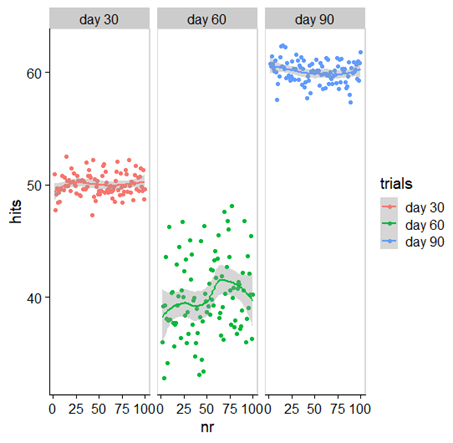
\includegraphics[width=4.16667in,height=\textheight,keepaspectratio]{images/MotL_sim2.png}

}

\caption{\label{fig-simB}Simulation Leistung vs.~Lernen 2}

\end{figure}%

\textbf{MERKE: Verbesserungen entstehen aus Variabilität. Aufbrechen von
konstanten Mustern kann nur durch Auslenkung passieren.}

\section{Bildliches Lernen}\label{bildliches-lernen}

\subsection{Vorzeigen}\label{vorzeigen}

Eine Übung vorzuzeigen bedeutet vor allem \textbf{Lernen am Modell}. Die
Lernenden sehen die Bewegung und versuchen die
Bewegung/Bewegungsprinzipien zu imitieren. Ste-Marie und Kollegen
beschreiben 2012 ein generelles Modell zum Erlernen durch Beobachtung.
Sie fassen die bisherige Forschungen zusammen (Ste-Marie et al. 2012)
und überarbeiteten vor kurzem ein narratives Review dazu (Ste-Marie,
Lelievre, and St Germain 2020).

Um optimales Lernen am Modell zu erreichen, sollte das Modell \textbf{so
ähnlich wie möglich} zur lernenden Person sein. Ähnlichkeiten in Gender,
Alter oder Körpermaße sind relevant. Aber sogar die Expertise des
Modells kann einen Einfluss haben. So ist es für absolute Anfänger nicht
unbedingt vorteilhaft von einem Profi zu lernen, sondern von jemanden,
der/die nur leicht über ihrem Erfahrungslevel steht. Es zeigt sich sogar
manchmal, dass es Vorteile haben kann, wenn das Modell selbst noch
kleine Varianten oder Fehler macht, diese erkennt und versucht diese
auszubessern. Auch die Art wie das Modell über sein eigenes Können und
seine Verbesserungen spricht ist entscheidend.

Das sogenannte \textbf{Learning und} \textbf{Coping} \textbf{Modell},
das selbst noch lernt und ihre eigenen Schwierigkeiten und
Lernstrategien anspricht, hilft vor allem Lernenden selbst eine höhere
Zuversicht und Motivation gegenüber dem eigenen Lernprozess zu bekommen.
Ein \textbf{Skilled und} \textbf{Mastery Modell} (zeigt immer perfekte
Bewegungen und hat keine Zweifel am Können) auf der anderen Seite, führt
eher zu besserem motorischen Lernen aber unterstützt weniger die
self-efficacy.

Einer Person, die eher damit Schwierigkeiten hat zu glauben, dass sie
die Bewegung erlernen kann und daher motivationale Probleme hat, zeigt
die Trainerin ein ähnliches Modell, das am Anfang auch Probleme hatte
und langsam besser wird/wurde. Geht es rein um die technischen
Schwierigkeiten, ist es zumeist hilfreicher die „perfekte'' Ausführung
zu zeigen. Darüber hinaus kann aber ein Learning Coping Model auch
geeignet sein, um ein aktives Problem-lösen oder kreatives Handeln zu
forcieren. Noch erstaunlicher ist, dass Ste-Marie und Kollegen (2020)
beschreiben, dass bei Modellen, die der lernenden Person nicht ähneln,
ein Coping Model immer dem Mastery Model sowohl motorisch als auch
psychologisch überlegen ist! Bei der Beobachtung unterschiedlicher
Modelle sollte immer auf das Skill-Level der Person hingewiesen werden.

Hier sehen wir ein paar Probleme im Personal Coaching. Oft haben wir
Kund*innen, die uns als Trainer*innen sehr unähnlich sind (Alter,
Fitnesslevel, Geschlecht\ldots). Welche Strategien fallen dir ein um
dieses Problem zu minimieren?

\begin{itemize}
\tightlist
\item
  Kleingruppentraining
\item
  Zeigen der eigenen Leistungen
\item
  Videomaterial von anderen Übenden
\item
  Auf ausführliche Demonstrationen durch die PTs verzichten und andere
  Cues verwenden
\item
  Eigene Lernfelder und Lernprozesse aufzeigen
\item
  \ldots{}
\end{itemize}

\subsection{Lernunterstützung qualitative
Videoanalyse}\label{lernunterstuxfctzung-qualitative-videoanalyse}

Die Möglichkeit videounterstützt zu Arbeiten sollte genutzt werden. Bei
Verwendung von Smartphones sollten wir aber immer die Schwierigkeiten
des \textbf{Datenschutzes} beachten. Gerade auch in öffentlichen
Fitnessstudios sollte außerdem die Privatsphäre andere Besucher*innen
gewahrt werden! Bitte, lade keine Videos von anderen Personen (Klient*in
oder nicht) ungefragt auf öffentliche Plattformen hoch! Get your Ethics
straight Section~\ref{sec-ethikschuetzt}.

Die hier dargestellte Methode zur qualitativen Videoanalyse stützt sich
praktisch auf dem Buch \emph{Qualitative Diagnosis of human movement}
(Knudson 2013), wurden jedoch inhaltlich mit den neueren Ergebnissen von
Ste-Marie at al. (2020) und Grundlagenliteratur (Magill and Anderson
2021) verglichen.

Nimm immer mehrere Wiederholungen auf (5-8+). Achte darauf, dass die
ganze Person im Video zu sehen ist. Wenn du auch einfache
\textbf{quantitative Tools} einsetzen möchtest, achte auf
\textbf{Parallaxenfehler} (Figure~\ref{fig-Paralax}) und wähle einen
optimalen Winkel zur Analyse (90° zur Bewegungsrichtung). Die
Aufnahmefrequenz sollte nach dem Nyquist Theorem gestaltet sein (Siehe
Biomechanik und Sportinformatik Vorlesungen).

\begin{figure}

\centering{

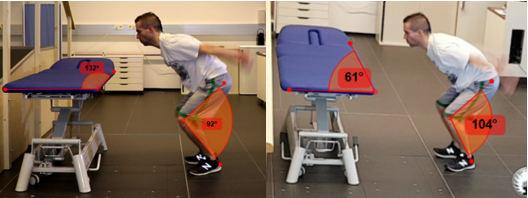
\includegraphics[width=4.16667in,height=\textheight,keepaspectratio]{images/MotL_Videoaufnahme.png}

}

\caption{\label{fig-Paralax}Winkel bei Videoaufnahmen}

\end{figure}%

Aus der Sicht des motorischen Lernens ist es wohl besser (wenige Studien
dazu), wenn das Video die Person frontal (\emph{objectiv view}) oder von
hinten (\emph{subjectiv view}) zeigt, nicht von der Seite oder einem
anderen Winkel. Aus praktischer Sicht sollte man sich hier jedoch vor
allem nach der gezeigten Bewegung und der Zielkorrektur richten.

Achte darauf, dass du die Aufnahme früh genug startest. Bei Kraftübungen
empfiehlt es sich auch die Vorbereitung und Nachbereitung der Übung zu
filme (aufheben und ablegen der Hanteln). Gerade in diesem Zeitfenster
passieren oft die ersten Fehler, die potentiell zu Verletzungen führen
können.

Die Kamera ist bei Bewegungsaufnahmen möglichst immer statisch! Daher
brauchst du zum Beispiel bei Laufübungen viel Abstand zwischen Kamera
und übender Person (bis zu 20m).

Es empfiehlt sich aus zwei Betrachtungswinkel zu filmen. In der Praxis
ist das meist schwierig. Wähle die wichtigste Ansicht zuerst. Dafür muss
dir im Vorhinein klar sein, worauf du deinen Coachee hinweisen möchtest.

Wenn du der Person das Video zeigst bietet sich folgendes Vorgehen an:

\begin{enumerate}
\def\labelenumi{\arabic{enumi}.}
\tightlist
\item
  Zeige erst das ganze Video in normaler Geschwindigkeit und ohne
  Kommentar. So kann die Person einen Überblick gewinnen und sich auf
  die Ansicht einstellen. (Manchmal kommt von Kund*innen als erstes „Oh
  Gott ,wie schau ich denn aus!{}``. Das ist nicht hilfreich, wenn es um
  Bewegungsqualität geht und du ihr eigentlich etwas erklären willst.
  Also lass der Person erst mal Zeit.)
\item
  Gib deinem Coachee dann konkrete Hinweisen dazu, auf was sie schauen
  soll. Denke daran - \emph{weniger ist mehr} -- und zeig ihr das Video
  noch ein paar Mal in normaler Geschwindigkeit und ohne Zoom.
  (Langzeitlernen lässt sich durch Hinweise wahrscheinlich nicht
  verbessern, aber es hilft Kurzzeit P zu verbessern).
\item
  Falls es noch notwendig ist, kannst du Zoom und Zeitlupe zu Hilfe
  nehmen, um auf deine Punkte oder auf Fragen genauer einzugehen. (Bei
  manchen Untersuchungen zu Krafteinsatz und optimalen Timing einer
  Bewegung stellt sich Slow-motion sogar als negativ heraus, bei
  komplexen Bewegungsabfolgen als positiv.)
\item
  Lass der Person etwas Verarbeitungszeit und lass sie dann die Bewegung
  nochmals probieren.
\item
  Wenn du ein zweites Modell hast, ist das in jedem Fall vorteilhaft
  dieses zusätzlich zu zeigen. Zum Beispiel kannst du deine Variante als
  \textbf{Skilled Model} zeigen. Achte darauf, dass beide Videos die
  gleiche Ansicht zeigen. Ob du sie dann übereinanderlegst oder
  nebeneinander präsentierst ist nicht so wichtig. Wenn du sie
  hintereinander zeigst, zeige sie möglichst abwechselnd.
\item
  Manche PTs geben den Trainierenden die Kameraaufnahme zum
  eigenständigen abspielen und zeigen gleichzeitig die Übung selbst,
  live vor. Dies scheint mir eine gute Strategie zu sein. Studien, die
  genau diese Variante verwenden sind mir nicht bekannt.
\item
  Lass deine Coachees selbst wählen wie oft sie videogestütztes Feedback
  bekommen. Dies scheint deutlich besser zu sein, als einer Person
  ungefragt Feedback Videos zu geben!
\end{enumerate}

\section{Lernstrategien -
Lernmodelle}\label{lernstrategien---lernmodelle}

\subsection{Implizites Lernen}\label{implizites-lernen}

In den letzten Jahrzehnten kamen implizite Lernstrategien gegenüber
expliziten mehr und mehr in Mode. In drei verbreiteten Lehrbüchern von
Magill (2021), Schmidt (2019) und Gollhofer (2012) wird implizites
Lernen als überlegen dargestellt und von den Author*innen für das
\textbf{Lernen von Bewegungsverhalten} empfohlen.

Implizites Lernen geht von der Idee aus, dass der anfänglich hohe
kognitive Aufwand zum Erlernen einer neuen Fertigkeit oder Fähigkeit
umgangen werden kann, indem von Anfang an auf \textbf{unterbewusste oder
automatisierte Strategien} gesetzt wird. Es wird daher zum Beispiel
nicht exakt beschrieben oder gezeigt, wie der Arm bei einer Bewegung
geführt wird. Anstelle dessen werden Bilder oder Analogien verwendet und
damit ein \textbf{externaler Fokus} und \textbf{Knowledge of Results}
gesetzt. Anstelle Übungen so zu gestellten, dass sie kognitiv analysiert
werden können und die Personen Zeit und Aufmerksamkeit auf einzelne
Aspekte setzen können, werden von Anfang an \textbf{Dual-Task} Aufgaben
gesetzt, die ein „Zerdenken'' der Bewegung verhindern.

Nach Meinung von 49 Expert*innen in einem Delphi Prozess ist jedoch
nicht klar, welche dieser Strategien wirklich mehr explizit oder mehr
implizites lernen aktivieren (Kleynen et al. 2014). Theoretisch sollte
es jedenfalls durch implizites Lernen schneller möglich werden, dass die
Übenden ein automatisiertes Bewegungsverhalten im Alltag oder im Chaos
eines Spiels umsetzen können (Figure~\ref{fig-ImpExp}).

\begin{figure}

\centering{


\includegraphics[width=4.16667in,height=\textheight,keepaspectratio]{Images/MotL_Kal2018.png}

}

\caption{\label{fig-ImpExp}Implizites vs.~Explizites Lernen (Kal et al.,
2018, 3/25)}

\end{figure}%

In einem systematischen Review zeigten Kal et al. (2018), dass implizite
Lernstrategien (vorrangig Analogien und externaler Fokus) Vorteile haben
können. Besonders im Sinne des Langzeitlernens zeichnen sich
Unterschiede ab. Die Studienlage ist jedoch sehr begrenzt und eine Risk
of Bias Analyse fiel hier unklar aus. Die Autoren beschränkten sich auf
das Maß der Automatisierung der Bewegung. Gollhofer und Kollegen (2012)
beschreiben ihrerseits viele Studien, die Vorteile von implizitem Lernen
zeigen, wenn es zum Beispiel zu Handlungen unter Ermüdung kommt. Masters
et al. (2020) beschreiben ebenfalls einige Vorteile für Personen mit
eingeschränkten kognitiven Fähigkeiten oder bei Kindern.

Insgesamt sind jedenfalls keine negativen Effekte durch implizite
Lernstrategien zu erwarten. Die meisten Abhandlungen von Expert*innen
raten stark zum Einsatz von implizitem Lernen, auch wenn systematische
Reviews scheinbar kaum vorhanden und mit spärlicher Evidenz aufwarten
können. Aus eigener Erfahrung bedarf es aber ein höheres Maß an
Expertise und Kreativität die Inhalte mit impliziten Lernstrategien
anzubieten.

Implizite Strategien {[}mastersAdvancesImplicitMotor2020{]}:

\begin{itemize}
\tightlist
\item
  Fehlerreduziertes Üben:

  \begin{itemize}
  \tightlist
  \item
    Übungen werden so leicht gestaltet, dass es kaum zu Fehlern kommt
    und die Übenden einfach die Bewegung machen können ohne zu denken.
    Dann erst werden die Übungen stufenweise erschwert
  \item
    Im Personal Coaching findet diese Methode wohl vorrangig bei
    koordinativen Übungen Einsatz. Aber auch bei higher-risk Übungen
    (Clean, Snatch\ldots) ist es wohl angebracht fehlerreduziertes Üben
    einzusetzen
  \end{itemize}
\item
  Analogien / mit mentalen Bildern arbeiten:

  \begin{itemize}
  \tightlist
  \item
    Es werden mentale Bilder (Tiere, geometrische Figuren, analoge
    Bewegungsmuster, Töne\ldots) eingesetzt um die Bewegung zu
    verdeutlichen
  \item
    Analogien sind aus meiner Erfahrung auch sinnvoll, weil sie gut
    erinnert werden können (und sie sorgen oft für ein paar Lacher im
    Training). Später reicht oft ein einzelnes Wort und die Klient*innen
    können die Übung nach dem mentalen Bild durchführen.
  \item
    Beispiele finden sich bei vielen der Oldschool Praktikern wie Pavel
    Tsatsouline oder Dan John. (Bankdrücken: „Brich die Stange'',
    Kniebeuge: „Zerreiße den Boden mit den Füßen!``, Single Leg RDL:
    „Wie eine Kinderwippe'', Kettlebell Snatch: „Reißverschluss
    zuziehen.'', Springen: „Lande wie eine Katze'' \ldots{}
  \end{itemize}
\item
  Externaler Fokus der Aufmerksamkeit:

  \begin{itemize}
  \tightlist
  \item
    Dieser Punkt wird von Masters unter implizites Lernen gesetzt.
    Gabriele Wulf, die viele der Studien durchgeführt hat, beschränkt
    sich jedoch nicht auf diese Einteilung.
  \item
    Unabhängig davon wurden viele Studien zu externalem Fokus
    durchgeführt und die Ergebnisse scheinen recht konsistent.
    Externaler Fokus ist für das Lernen fast immer besser als
    internaler!
  \item
    Es wird dabei nicht der Fokus auf den Körper oder die Bewegungen des
    Körpers gelenkt, sondern auf äußere Effekte der Bewegung oder auf
    Instrumente.
  \item
    Z.B. Langhantel Press: Internal = „Streck die Arme''; „Spann den
    Trizeps'', External = „Drück die Hantel zur Decke''
  \end{itemize}
\item
  Dual Task Learning:

  \begin{itemize}
  \tightlist
  \item
    Hier werden von Anfang an Dual Task Aufgaben eingebaut.
  \item
    Dies macht aus meiner Sicht besonders dann Sinn, wenn Personen
    Übungen unaufgefordert „zerdenken''. Gleichgewichtsübungen können
    zum Beispiel manche Personen mental sehr fordern. Sie beginnen über
    die richtige Beinachse oder das Fußgewölbe nachzudenken (=meist
    internaler Fokus). Um das zu verhindern könnten zusätzliche
    motorische oder kognitive Aufgaben gestellt werden (miteinander
    reden, einen Ball zuwerfen\ldots).
  \end{itemize}
\end{itemize}

\subsection{Explizites Lernen}\label{explizites-lernen}

Seit Jahrzehnten werden von führenden Denkern im Bereich Motor Control
und Motor Learning Modelle vorgeschlagen, die Stufen des Lernens
beschreiben. Diese basieren zumeist auf einem \textbf{expliziten
Lernmodell}. Eine Einstufung hat in der Praxis den Vorteil, dass
möglicherweise erkennbar wird wann welches Verhalten und welche
Verbesserungen eintreten. Es hilft uns auch die richtige Lehrstrategie
zu wählen. So beschreiben schon Fitts und Posner 1967 ein dreistufiges
Modell, das von einer \textbf{Kognitiven}, einer \textbf{Assoziativen}
und einer \textbf{Autonomen/Automatisierten} \textbf{Phase} spricht. Die
beschriebenen Strategien zum Erlernen decken sich Großteiles mit
modernen Ansätzen.

\begin{figure}

\centering{


\includegraphics[width=4.16667in,height=\textheight,keepaspectratio]{Images/MotL_Spampinato2021.png}

}

\caption{\label{fig-Spampinato}Heat map of Learning Strategies
(Spampinato \& Celnik, 2021, p.~247)}

\end{figure}%

Aktuell unterscheidet man vier Lernstrategien im expliziten Lernen
(Spampinato and Celnik 2021):

\begin{itemize}
\tightlist
\item
  Error Based Learning:

  \begin{itemize}
  \tightlist
  \item
    Fehler erkennen und korrigieren. Ist besonders am Anfang der
    Lernphase wichtig und führt zu schnellen (jedoch weniger
    dauerhaften) Verbesserungen
  \item
    Führt zu hoher Variabilität der Ausführung
  \item
    Wiederholtes, direktes Feedback für Anfänger*innen ist die Methode
    der Wahl
  \item
    Das Feedback sollte direkt durch das Ergebnis erfahrbar sein, da es
    auch um quantitative Abweichungen geht (wie weit ist der Ball
    daneben geflogen)
  \end{itemize}
\item
  Use-Dependent Learning:

  \begin{itemize}
  \tightlist
  \item
    Am besten zu beschreiben durch den bekannten Spruch „practice makes
    permanent''
  \item
    Wiederholen von Bewegungen führt zum „einschleifen''. Dadurch wird
    die Strategie vermehrt eingesetzt.
  \item
    Selbst bei Fehlern wird die Bewegung nicht korrigiert
  \item
    Sollte erst in einer späteren Phase des Lernens, wenn die Bewegung
    bereits zu einem hohen Maße beherrscht wird, eingesetzt werden. Es
    führt dann jedoch zu höherer Präzision, Automatisierung und
    geringerer Reaktionszeit. Das ist notwendig im Sport und für das
    Entstehen von \textbf{Flow} \textbf{Erlebnissen.}
  \end{itemize}
\item
  Reinforcement Learning:

  \begin{itemize}
  \tightlist
  \item
    Die Person muss Bewegungen erforschen, um die besten Erfolge zu
    finden und versucht diese dann zu reproduzieren.
  \item
    Durch das Erkennen von erfolgreichen Wiederholungen kommt es zu
    geringerer akuter Verbesserung, aber das Behalten
    (\textbf{retention}) ist dafür länger als beim Error based learning.
  \item
    Positive Verstärkung bei gelungenen Bewegungen ist die Methode der
    Wahl. Die Wichtigkeit der Methode steigt mit dem Grad des
    Fortschritts der lernenden Person
  \end{itemize}
\item
  Strategy Learning:

  \begin{itemize}
  \tightlist
  \item
    Kognitive Prozesse in Bezug auf die Übung/Bewegung. Trainierende
    müssen Bewegungsabfolgen verstehen, verinnerlichen und Abrufen und
    oft auch mehrere Bewegungen gleichzeitig starten.
  \item
    Die richtige Sprache und das Verwenden von Schlüsselwörtern/-phrasen
    sind die richtige Strategie zur Unterstützung.
  \end{itemize}
\end{itemize}

\subsection{Update (08-2024)}\label{update-08-2024}

Mögliche zukünftige Updates sollten die aktuelle Diskussion und Evidenz
berücksichtigen (z.B. \href{https://peerj.com/articles/17718/}{Nevo et
al., 2024}).

\section{Organisationsformen im Motorischen
Lernen}\label{organisationsformen-im-motorischen-lernen}

Wie im S\&C Training, gibt es auch beim Lernen die Möglichkeit für
längere Zeit bei einer Übung zu bleiben (\textbf{geblocktes üben}),
Übungen abwechselnd oder in einer Art Zirkel zu machen
(\textbf{serielles üben} Figure~\ref{fig-seriell}) oder die Übungen in
zufälliger Reihenfolge zu machen (\textbf{randomisiertes üben}).
Vielleicht hast du nach all den Informationen schon eine Idee wie sich
welche Form auf die akute P und auf langzeitiges L (retention und
transfer) auswirken könnte\ldots{}

Es zeigt sich fast uneingeschränkt, dass serielles und randomisiertes
üben zu besseren Retention und Transfer-tests führt (= besseres lernen).
Geblocktes lernen führt zu höherer akuter Leistung (Wright and Kim
2020). Diese Erkenntnis ist für Trainierende oft schwer vorstellbar.
Viele motivierte Kund*innen, die Übungen ganz genau lernen wollen,
halten es für wichtig lange und ganz intensiv beim Coaching einer Übung
zu bleiben. Es bedarf manchmal einer Erklärung dazu, dass zufälliges
auswürfeln der nächsten Übung der beste Weg wäre, um sich die Ausführung
aller Übungen zu merken.

\begin{figure}

\centering{

\pandocbounded{
\includegraphics[keepaspectratio]{Images/MotL_Seriell.png}}

}

\caption{\label{fig-seriell}Feedback bei seriellem Üben}

\end{figure}%

Spätestens hier sollte dir auch auffallen, dass Empfehlungen für
optimales \textbf{Training} (zum Beispiel Stationstraining für
Muskelaufbau) nicht unbedingt mit Empfehlungen für \textbf{motorisches
Lernen} übereinstimmen. Als Personal Trainer*in ist es also deine
Aufgabe dir zu überlegen was für individuelle Klient*innen in der
aktuellen Situation der wichtigere Faktor ist. Darüber hinaus soll
gesagt sein: auch randomisiertes Training kann Muskeln aufbauen und auch
Block Üben kann Lernen anregen.

\section{Feedback -- aber wie viel}\label{feedback-aber-wie-viel}

Nach erfolgreicher Bewegungsausführung geben Coaches Feedback zur
gelungenen Technik, um so ein besseres Lernen zu gewährleisten (und
ihren Job zu rechtfertigen 😉). Jedoch bekommen Trainierende nicht nur
durch die Trainer*in Rückmeldung. Erstens bekommen die Klient*innen
Feedback über die erbrachte externe Wirkung, die sie erzeugt haben.
Wurde das Gewicht bewegt, wurde die geforderte Arbeit am Ergometer
gefahren, stehe ich noch immer einbeinig auf dem Wackelkissen\ldots{}
Dies wird als \textbf{knowledge of results} bezeichnet. Zweitens
bekommen sie Feedback durch ihren Körper. Hier gilt leider oft die
Devise des Körpers: „Nichts gesagt ist Lob genug''. Denn dieser meldet
sich mittels Schmerzen nur dann, wenn etwas nicht stimmt. Geübte
Trainierende bekommen aber auch ein Gefühl dafür, wenn sich eine
Bewegung gut anfühlt. Sie verleihen diesem Gefühl auch verschiedenartig
Ausdruck: die Bewegung fühlt sich dann zum Beispiel \emph{rund, weich}
oder \emph{einfach} an. Dies wird als \textbf{knowledge of performance}
bezeichnet. Der Job der PTs ist es diese Art des eigenen Feedbacks zu
verbessern, indem sie zusätzliche Rückmeldungen anbieten. Dieses äußere
Feedback soll aber das innere Feedback nicht ersetzen, sondern eben
helfen das innere Feedback zu verstehen.

Praktische Zusammenfassung von Feedbackgabe nach Grundlagen des
motorischen Lernens:

\begin{itemize}
\tightlist
\item
  Weniger ist mehr (Guidance Hypothese nach Schmidt)

  \begin{itemize}
  \tightlist
  \item
    Diesen Rat geben alle Grundlagenwerke, die bisher zitiert wurden.
    Gerade für Retention- und Transfertests ist es wahrscheinlich
    vorteilhaft weniger, geblocktes Feedback, und mit zunehmenden
    Leistungslevel immer weniger zu geben.
  \item
    Eine umfangreiche Meta-analyse (McKay et al. 2022) versuchte genau
    diese Hypothesen zu testen. Die Analyse von McKay fand ein sehr
    breites 95\%CI für die gepoolten Effekte und es scheint einige
    Covariaten zu geben, die zu unterschiedlichen Effekten führen. Diese
    wurden aber in der Analyse nicht eindeutig identifiziert. Der wahre
    Effekt liegt also weiterhin im Dunkeln. Für Praktiker*innen reicht
    bis auf weiteres: Weniger ist mehr!
  \end{itemize}
\item
  Lass die Übenden aktiv Feedback einfordern

  \begin{itemize}
  \tightlist
  \item
    Auch dieser Rat zieht sich durch die gesamte Literatur. Feedback zu
    ziehen, verbessert jedoch nicht nur das motorische Lernen. Es ist
    ist auch ein entscheidender Faktor in den Bereichen
    Selbstwirksamkeit, Selbstbild und Motivation. Lass also deine
    Kund*innen entscheiden wann und wie oft du Rückmeldung gibst.
  \end{itemize}
\item
  Zeitlich muss Feedback nicht sofort gegeben werden. Lass erst Lernende
  selbst über die Leistung reflektieren.
\item
  Passe die Präzision des Feedbacks an das Leistungslevel an
  (\textbf{Bandwidth Feedback}).

  \begin{itemize}
  \tightlist
  \item
    Einzelne Studien zeigen, dass zu hohe Präzision im Feedback
    überfordert. Wenn die Wiederholungen in einem guten Rahmen sind,
    reicht es dies zu bestätigen/verstärken. Liegt eine Abweichung vor
    reicht oft „zu weit''/``zu viel'', anstatt präzisen Angaben. Diese
    kommen erst bei Fortgeschrittenen in Spiel.
  \item
    Auch dieser Punkt wurde bei McKay et al. (2022) miteinbezogen und
    konnte nicht voll bestätigt werden.
  \end{itemize}
\item
  Gib mehr positives Feedback als negatives. (Was ist gelungen vs.~Was
  ist nicht gelungen)
\item
  Mische \textbf{Knowledge of Results} mit \textbf{Knowledge of
  Performance}
\item
  Richte einen externalen Fokus der Aufmerksamkeit
\item
  Identifiziere die kritischen Punkte der Übung
\item
  Geblocktes Feedback über mehrere Wiederholungen
  (Figure~\ref{fig-block}) ist oft gleichwertig oder besser als Feedback
  nach jeder Wiederholung.
\end{itemize}

\begin{figure}

\centering{


\includegraphics[width=4.16667in,height=\textheight,keepaspectratio]{Images/MotL_Block.png}

}

\caption{\label{fig-block}Feedback bei Block-üben}

\end{figure}%

Hier erscheint in Kürze: ``Lernen unter Ermüdung'' und ``Schlaf und
Motorisches Lernen''

\section{Weiterführende Literatur}\label{weiterfuxfchrende-literatur}

Eine praxisorientierte Zusammenfassung mit wunderbaren Bildern und
Coaching Cues findet sich bei
\href{https://www.thelanguageofcoaching.com/}{Nick Winkelman -- The
Language of Coaching}.

\section{Literatur}\label{literatur-9}

\bookmarksetup{startatroot}

\chapter{Trainingsplanung und -steuerung im Personal
Training}\label{sec-trainingsplanung}

Trainingswissenschaft und Trainingslehre sind eine der umfangreichsten
Unterrichtseinheiten in den meisten Personal Training Ausbildungen.
Warum nicht in diesem Kurs?

Der wichtigste Grund dafür ist, dass angenommen wird, dass Du als
Student*in der Sportwissenschaft bereits umfangreiches Wissen in anderen
Lehrveranstaltungen gesammelt hast. Aus Erfahrung interessieren sich die
meisten Sportwissenschafter*innen ohnehin stark für Trainingslehre, die
im Selbststudium über durch Bücher, Kurse, Videoplattformen und
Eigenerfahrung recht „leicht'' erlernt werden kann. Selbst Laien können
sich heute schnell das wichtigste Wissen um Übungsausführung und
Trainingsplanung aneignen. Wahrscheinlich ist die Trainingssteuerung
jener Zweig, der schwieriger zu beherrschen ist und zu dem auch weniger
frei zugängliche Information im Netz zur Verfügung steht.

Was sind die Ziele dieses Kapitels?

\begin{itemize}
\tightlist
\item
  Kritisches Hinterfragen der gängigen Planungskonzepte für Personal
  Training
\item
  Herunterbrechen von Zielen der Kund*innen auf die kleinste
  Organisationseinheit in der Planung: einzelne Trainingseinheiten
\item
  Üben einen Trainingsplan zu erstellen und anzuwenden
\item
  Wie kann ich Fortschritte sichtbar machen? -- reliable, objektive und
  valide Testungen
\end{itemize}

\section{Kritisches Auseinandersetzen mit bekannten
Trainings-Prinzipien}\label{kritisches-auseinandersetzen-mit-bekannten-trainings-prinzipien}

In diesem Unterkapitel spielen wir \emph{advocatus diaboli} und nehmen
uns ein paar der weit verbreiteten Trainingsprinzipien genauer unter die
Lupe.

\subsection{Testen und Messen -- kritisch
hinterfragen}\label{testen-und-messen-kritisch-hinterfragen}

Eine fast universelle Regel ist, dass Trainer*innen möglichst präzise
und akribisch den Ist-stand der Trainierenden testen sollen, um daraus
die Trainingsplanung zu gestalten. Nach einer angemessenen Zeit werden
die Variablen wieder bewertet.

Warum sollten wir deiner Meinung nach Ziele objektivierbar machen, um
dann zeitlich wiederholte Testungen durchzuführen?

Mit den Worten des viel vergötterten Managers Peter Drucker: „What gets
measured gets managed''.\footnote{Peter Drucker hat das übrigens
  wahrscheinlich nie gesagt und dieser Artikel
  \url{https://www.drucker.institute/thedx/measurement-myopia/}
  beschreibt ein ganz anderes Bild. Aber Peter Druck, Albert Einstein
  Buddha und Warren Buffet kassieren wohl viele falsche Zitate .} Dies
wird auch auf den Umgang mit Menschen umgelegt -- egal ob bei
Bildungszielen und vergleichbaren Bildungstests (siehe Zentralmatura),
in der Reha oder im Training (Spiroergometrie, Krafttests,
Körperzusammensetzung\ldots). Überall folgen wir der Leitidee nach
Drucker. Daraus ergibt sich aber auch im Umkehrschluss eine mögliche
Verzerrung der Inhalte, Ziele und der Interpretation der Ergebnisse.
Denn es verbessert sich auch nur das was wir messen. Alles was Training
kann und nicht gemessen wird, wird abgewertet oder wird völlig aus den
Augen verloren. Was passiert also mit den Kund*innen die „einfach
fitter'' werden wollen. Wir als Trainer*innen münzen dies jedoch um auf
die Verbesserung der 5Rm Kniebeugen und des 2000m Ruderergometertests?

Wenn sich die Kund*innen schließlich darin auch wirklich verbessern,
sind sie zumindest zufrieden. Verbessern sie sich nicht, haben aber
endlich Freude an Bewegung gefunden, Blutwerte und Schlaf sind
verbessert, können sie diese Änderung nicht wahrnehmen. Was nicht
gemessen wurde, wurde mental diskreditiert und fällt nicht auf.

Für die folgende Übung bitte ich dich, dass du alle Wirkungen
niederschreibst, die ein gutes Training auf einen Menschen haben kann.
Mach dir keine Sorgen, wenn du nicht die aktuelle Evidenzlagen dazu
kennst und dir nicht unsicher bist. Probiere es einfach mal aus - Was
kann Training alles bewirken?

Hast du alles? Hier noch ein paar Denkanstöße: Herzkreislaufsystem
(Herz, Blutgefäße, Blut), Stoffwechsel, Immunsystem, Bewegungsapparat
(Knochen, Sehnen, Muskeln, Faszien), Psychisches (Kognition, Emotionen,
Selbstbild\ldots), Schmerzverarbeitung, Soziales, Schlaf,
Körperzusammensetzung, äußeres Erscheinungsbild, selbst wahrgenommenes
Erscheinungsbild, \ldots{}

Ok, wenn du dir etwas Zeit genommen hast, dann sollte deine Liste
ziemlich lang sein. Nun, wieviel davon kannst du als Trainer*in
realistischerweise, mit dir zugänglichem Equipment messen? Nicht gerade
viel, oder?

Das Problem entsteht damit auf zwei Ebenen. Zum Ersten bedeutet das,
dass wir notgedrungen unsere Trainingsprinzipien und -pläne auf jene
Dinge ausrichten, die wir einfach messen können. Andere Ebenen bleiben
unterrepräsentiert und in der Praxis (teilweise auch in der Forschung)
weniger bekannt. Manche Dinge können wir mit subjektiven Skalen gut
abdecken. Das funktioniert aber auch nur in jenen Bereichen, in denen
subjektive Empfindungen auch entscheidende Outcomes sind (z.B.
Gelenksverscheiß vs.~Schmerzen im Gelenk).

Zweitens bedeutet das auch für Trainierende, dass ein Training (oder
allgemein Bewegung) nur dann effektiv und hilfreich ist, wenn es diese
messbaren und sichtbaren Variablen verändert. Wir verändern als
Trainer*innen und Forscher*innen den Fokus der Gesellschaft durch unsere
Messungen. Wenn alle Praktiker*innen ihre Trainings mit „verringerter
Bauchumfang'' auf ihrer Homepage bewerben, so wird dies zum
entscheidenden Outcome durch Training.

Dazu kommt noch die Schwierigkeit, dass die Effektivität von Training
(auf die gemessenen Outcomes) individuell und zeitlich sehr variabel
ist. Die Frage nach Trainierbarkeit einzelner Individuen ist noch lange
nicht vollständig geklärt. Aber es kann angenommen werden, dass sich der
Anteil der non-responder \footnote{Ich verwende hier bewusst den Begriff
  Non-Responder aus reinem Pragmatismus und um die Problematik noch
  klarer darzustellen. Es geht um für die gemessenen Variablen in einem
  relevanten Zeitraum! In Wahrheit sollte \emph{responsivness} nicht als
  fixer Bestandteil einer Person (\emph{trait}) sondern wohl eher als
  ein zeitlich begrenzter und auf einen Faktor bezogenen Zustand
  (\emph{state}) betrachtet werden.} im zweistelligen Prozentbereich
befindet (Bouchard et al. 2012; M. Roberts et al. 2018).

Nicht alle deine Kund*innen werden also durch das Training, das du ihnen
bieten kannst auch wirklich Verbesserungen erzielen. Jedoch kann es sehr
wohl sein, dass Personen in anderen, nicht gemessenen Bereichen
Verbesserungen erzielen(Bouchard et al. 2012; Karavirta et al. 2011;
Radak and Taylor 2021).

Die Frage ist dementsprechend, ob wir Training an sich nicht auch falsch
vermarkten!

Natürlich brauchen wir weiter Anhaltspunkte für unsere
Trainingssteuerung. Wenn keine gewünschten Ergebnisse erzielt werden,
sollten wir nicht automatisch davon ausgehen, dass es sich hier um
reduzierte Anpassungsfähigkeit handelt. Zuerst sollten wir immer nach
Verbesserungen im Training oder in anderen Zubringersystemen (Ernährung,
Regeneration) suchen. Gleichzeitig ist es wichtig, dass wir unseren
Klient*innen neben der Verringerung des Bauchumfangs oder der
verbesserten Bankdrückleistung auch andere Marker für Verbesserung
anbieten können.

Alternativ können wir beginnen alles zu messen und zu tracken, was uns
möglich ist und nach angemessener Zeit betrachten was sich verbessert
hat. Dieser Ansatz ist für die Trainer*innen ein sehr praktischer und
bietet sich wunderbar an, um die Markttrommel zu schlagen. Durch die
Verbreitung von Wearables und Tracking-Devices wird dies auch immer
einfacher. Auch diese Handlungsweise hat ihre Tücken. Messen wir
möglichst viele Variablen können wir sicher sein, dass sich irgendeine
verbessern wird. Leider liegt das dann nicht unbedingt an einem
erfolgreichen Trainingsprozess, sondern entsteht durch Zufall. Dieser
Gefahr setzten wir uns besonders aus, wenn wir auch kleine
Verbesserungen sofort als relevant werten. Wir sollten zumindest a
priori einen minimalen messbaren und relevanten unterschied festlegen
(Franco et al., 2016). Nur wenn sich unserer Kund*innen darüber hinaus
verändern, sollten wir von einer „echten'' Anpassung ausgehen. Anders
entsteht daraus eine sehr unehrliche Praxis.

Wie denkst du, können wir vorgehen? Findest du einen optimalen Weg
zwischen \emph{alles testen} und \emph{nichts testen} und ins Blaue
hinein trainieren?

Eine Lösung des Problems ist, sich nochmal neu zu überlegen, wie Ziele
definiert werden und wie wir mit Klient*innen über das Erreichend dieser
Ziele sprechen. Es ist eine schwierige Angelegenheit, aber die
ehrlichere Variante. Wir können die letztendliche Anpassung der
Kund*innen nicht vorhersehen und sollten solche Anpassungen auch nicht
als Ziele definiere (outcome goas). Die Ziele werden vielmehr als
Handlungen (process goals) definiert. Darüber haben wir mehr Kontrolle
und diese sollten auch gemessen und gemanaged werden. Wenn dies für alle
Beteiligen klar ist, können Trainingsleistungen trotzdem „on the fly'',
also während dem Training und nur zum Zweck der Trainingssteuerung
gemessen werden. Es werden also keine spezifischen Tests durchgeführt,
die den Trainingsprozess unterbrechen, Zeit und Ressourcen kosten und
oft hoch belastend sind. Anstelle dessen werden Daten währende dem
Training erhoben.

\subsection{Periodisierung im Personal
Coaching}\label{periodisierung-im-personal-coaching}

Eine der einflussreichsten und universellsten Theorien im Training ist
die Periodisierung von Trainingsinhalten. Aufbauend auf den Konzepten
der Stressreaktion nach Hans Selye (1975), hat sich die
Trainingswissenschaft ein Modell zurechtgezimmert, das von Ermüdung und
Erholung des Organismus ausgeht (Cunanan et al., 2018). Darauf aufbauend
werden durch zyklisches planen und steuern von Training versucht, eine
optimale Anpassung und Leistungsspitzen termingerichtet zu erreichen.
Dies wird als \textbf{Periodisierung} bezeichnet. Darunter seht die
Steuerung der einzelnen Elemente (Übungen und Belastungsparameter), was
als \textbf{Programming} bezeichnet wird (Bompa 2019; Cunanan et al.
2018; Stone et al. 2021). Für einen Versuch der Begriffsdefinition siehe
Figure~\ref{fig-peridprogram}.

\begin{figure}

\centering{

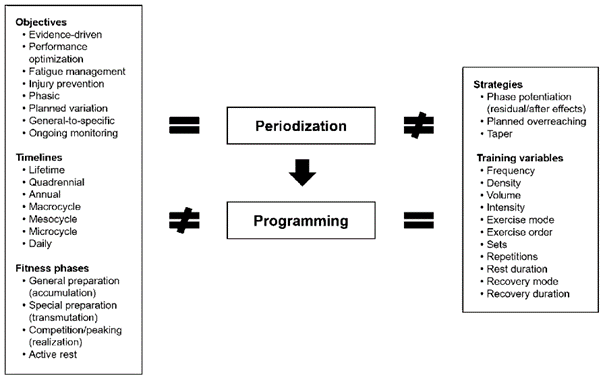
\includegraphics[width=4.16667in,height=\textheight,keepaspectratio]{images/PeriodProgram_Cunanan.png}

}

\caption{\label{fig-peridprogram}Periodisierung vs.~Programming: Was
genau Periodisierung eigentlich ist, scheint nicht so klar zu sein und
Kritiker und Befürworter liefern sich eine Schlacht über die
Nomenklatur. Einen Versuch der Klärung bieten Cunanan et al.~(2018)}

\end{figure}%

Aufbauend auf diesem Gerüst, das immer wieder konzeptuelle Kritik
erfährt (Buckner et al. 2017; Kiely 2018), haben Trainer*innen und
Wissenschafter*innen Prinzipien erstellt, um Training effektiver zu
machen. Besonders Arbeiten aus dem Kontext olympischer Sportarten haben
dabei unser Handeln geprägt (v.a. bekannt durchfig-peridprogram Matveyev
und Issurin, siehe Hornsby et al. 2020). Zusammenfassende
Übersichtsarbeiten fallen gemischt aus. In aktuelle Reviews zeigt sich
Periodisierung für Kraftverbesserungen zwar als vorteilhaft, für
Muskelaufbau jedoch weniger entscheidend (Moesgaard et al. 2022;
Williams et al. 2017). Für Ausdauertestungen könnte es wieder Vorteile
durch spezielle Periodisierungsmodelle geben (Mølmen, Øfsteng, and
Rønnestad 2019). Die wissenschaftliche Datenlage zu Periodisierung ist
insgesamt überraschend überschaubar. Kritisiert wird außerdem, dass
Ergebnisse vor allem durch den Effekt von „Training näher am Test''
entstehen (Kiely 2018; Nunes et al. 2018). Wenn also
Periodisierungsmodelle nur für Testergebnisse bzw. Wettkämpfe
vorteilhaft sind, ist es dann überhaupt sinnvoll für Klient*innen im
Personal Coaching ein Periodisierungskonzept aufzubauen?

Eine Struktur und zeitliche Abfolge geplanter Trainingsinhalte und
Methoden ist meiner Meinung nach sinnvoll um (1) einzelne Strukturen und
Systeme vor Überlastung zu schützen, (2) das Training abwechslungsreich
zu gestalten und (3) Verbesserungen sichtbarer zu machen.

Der erste Punkt ist ein sehr verbreitetes Argument für Periodisierung
und ergibt sich auch aus den Modellen, wie sie in der Basisliteratur
aufzufinden ist. Verschiedene Strukturen brauchen unterschiedlich lange,
um sich zu regenerieren. Eine Trainingspause zwischen Belastungen soll
vermeiden, dass zum Beispiel passive Strukturen überlastet werden. So
werden Periodisierungsmodelle nicht nur im Spitzensport, sondern auch
für Hobbyathleten (Leseempfehlung Boullosa et al. (2020)) oder in der
Reha (Kakavas et al. 2021) empfohlen.

Gerade bei Trainingsanfänger*innen mit hoher Motivation kann es
vorkommen, dass sie sich zu schnell zu viel zumuten. Es benötigt keinen
fein justierten Plan für jeden Mikrozyklus über die nächsten zwölf
Wochen. Jedoch sollten wir Klient*innen von Anfang an ein Verständnis
für kontinuierlichen, progressiven Trainingsaufbau vermitteln. So können
wir mögliche Überlastungen vermeiden. Einfache graphische Darstellungen
der Inhalte und eine kurze Erklärung dazu sind ausreichend, um den
Trainierenden ein Gefühl von Sicherheit zu geben.

Stone und Kollegen (Hornsby et al. 2020; Stone et al. 2021) gehen in
mehreren Artikeln gegen die Kritiken am Konzept der Periodisierung vor.
Ein Argument der Autoren ist, dass die experimentellen Vergleichsstudien
oft nicht der realen Applikation entsprechen. Sie sind ihrer Meinung
nach viel zu kurz, um Unterschiede in den Trainingsanpassungen zwischen
Periodisierungsmodellen zu zeigen\footnote{Zum Thema interne
  vs.~ökologisch Validität soll hier nochmal auf Kapitel 2
  Organisationsformen verwiesen werden. Dort ist uns diese Schwierigkeit
  schon begegnet als wir Personal Training mit eigenständigem Training
  nach Plan verglichen haben.}. Weiters geben sie an, dass die
Bezeichnung „Periodisierung'' oft falsch Verstanden wird (siehe auch
Cunanan et al., 2018 und Abbildung 1). In einem Punkt sind sich Kritiker
und Befürworter von klassischer Periodisierung einig: Es ist nicht
möglich dauerhaft in Topform zu sein! Daher wird in den
Periodisierungsmodellen versucht, einen Leistungspeak zu einem vorher
festgelegten Zeitpunkt zu schaffen. Diese Argumentation fällt jedoch für
die meisten Gesundheitssportler*innen flach.

\bookmarksetup{startatroot}

\chapter{Trainingsplanung und Gestaltung aus Sicht des
PTs}\label{trainingsplanung-und-gestaltung-aus-sicht-des-pts}

Da nun ein paar Konzepte kritisch beleuchtet wurden möchte ich auf
mögliche Lösungsvorschläge eingehen. Manche davon wurden aus der
Literatur entnommen. Andere sind aus meiner Erfahrung oder aus dem
Austausch mit Kolleg*innen gewachsen. Natürlich wird weiter spezifisch
auf die unterschiedlichen Evidenzlagen eingegangen.

\section{Übergeordnete Denkmodelle}\label{uxfcbergeordnete-denkmodelle}

Bitte behalte die beiden führenden Modelle der Evidenzbasierten Medizin
(EBM) und des Bio-Psycho-Sozialen (BPS) Sicht im Hinterkopf
Section~\ref{sec-BPS}, Section~\ref{sec-EBM}. Sie leiten uns durch die
Auswahl der Trainingsmethoden und Inhalte Figure~\ref{fig-EBM_BPS}.

\begin{figure}

\centering{

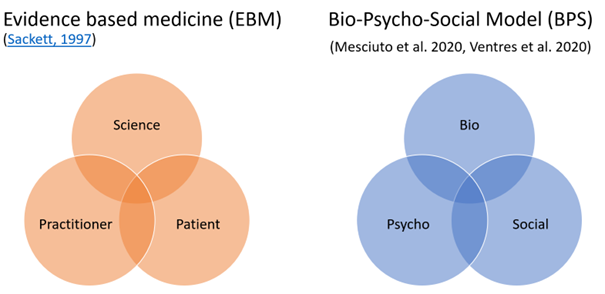
\includegraphics[width=4.16667in,height=\textheight,keepaspectratio]{images/EBM_BPS.png}

}

\caption{\label{fig-EBM_BPS}Grundlegende Modelle EMB \& BPS}

\end{figure}%

Das EBM Modell besagt, dass alle drei Pfeiler gleich stark gewichtet
werden sollen. In der Anwendung der Trainingsplanung soll diese so
aussehen, dass wir unsere Trainingspläne grundsätzlich nach den
Ergebnissen der wissenschaftlichen Forschung erstellen. Wir richten uns
nach Meta-Analysen, Systematischen Reviews, Guidelines, RCTs,
non-Randomized Trials und Cross-Sectional Studies (möglichweise in der
Reihenfolge, vergleiche dazu die Evidenzpyramide Abbildung 2, die in
unterschiedlicher Form veröffentlicht, kritisiert und überarbeitet wurde
(Mulimani 2017; Murad et al. 2016; Walach and Loef 2015)).

\begin{figure}

\centering{

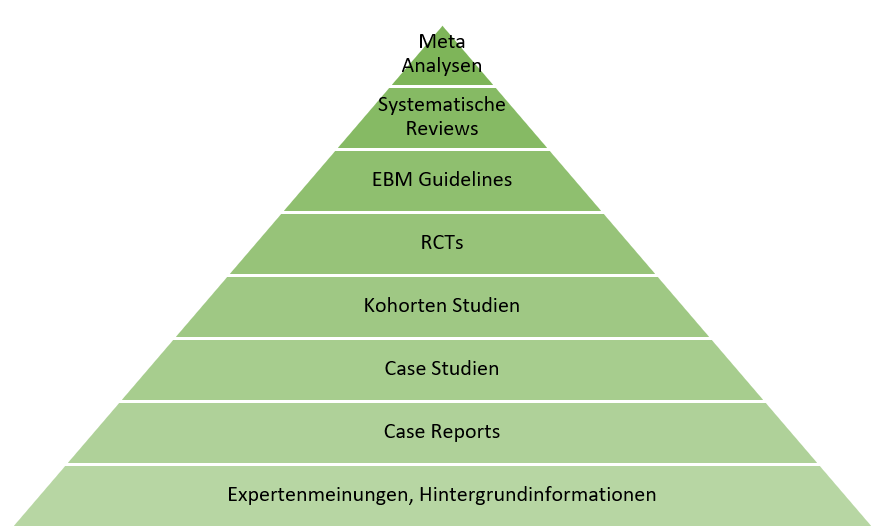
\includegraphics[width=4.16667in,height=\textheight,keepaspectratio]{images/Evidenzpyramide.png}

}

\caption{\label{fig-evidenzpyramide}Evidenz Pyramide (verbreitet z.B.
Cochrane Institute, Zugriff 2023
(\url{https://rehabilitation.cochrane.org/sites/rehabilitation.cochrane.org/files/uploads/sosort_dubrovnik_-_cochrane_reviews.pdf})}

\end{figure}%

Unser erster Entwurf eines Trainingsplans sollte sich also immer nach
dieser Pyramide (oder einem anderen, gut erprobten Modell) richten. Es
entsteht daraus häufig ein recht generischer Trainingsplan, der
generellen Vorgaben (z.B. jenen der WHO Bull et al. 2020) folgen sollte.
Wie oben bereits kurz angesprochen bilden die meisten Studien (und vor
allem Übersichtsarbeiten, die ja unsere primären Quellen sein sollen)
nur die Wirkung auf den „\emph{Durchschnittsmenschen}'' ab. Dieser
\emph{Durchschnittsmensch} ist jedoch ein Konstrukt und eine
statistische Illusion! Das folgende Beispiels soll das veranschaulichen:

Das erste Bild (Abbildung 3) zeigt ein typisches Ergebnis aus einer
Trainingsstudie. Man sieht, dass sich die Probanden im Schnitt eindeutig
verbessert haben. Es gibt auch ein paar Ausreißer nach oben und unten,
aber im Grunde ergibt sich eine erfolgreiche Intervention. In diesem
Fall ist das Ergebnis der n = 100 Personen mit einem gepaarten T-Test
hoch signifikant (p\textless0.001) und zeigt eine für Trainingsstudien
typische Effektgröße von d = 0.96, 95\% CI {[}1.25, 0.67{]}.

\begin{figure}

\centering{


\includegraphics[width=4.16667in,height=\textheight,keepaspectratio]{12-Programing_files/figure-pdf/fig-TrainingBoxplot-1.pdf}

}

\caption{\label{fig-TrainingBoxplot}Simuliertes Trainingsergebnis von
100 Probanden als Boxplot}

\end{figure}%

Das zweite Bild (Figure~\ref{fig-TrainingBoxplot}) zeigt das Ergebnis
jedoch auf individueller Ebene. Ungefähr 20\% der Proband*innen zeigen
keine Verbesserung oder sogar eine Verschlechterung. Im Normalfall haben
wir auch keine gute Erklärung dafür, warum es zu so einem Unterschied
kommt. Vielleicht gibt es Unterschiede in der Ernährung, im
Schlafverhalten, genetisch Unterschiede, etc. Selbst wenn die Studien
alle diese Daten erheben würden, wäre es statistisch jedoch nicht leicht
den echten Grund zu erfahren. Das hängt vor allem mit der geringen
Stichprobe zusammen, die wir meist in der Forschung zu Bewegung und
Sport finden. In Meta-Analysen und Systematischen Reviews verschwimmt
der Unterschied zwischen einzelnen Individuen deutlich mehr. Hier werden
schließlich auch leicht unterschiedliche Stichproben, Trainingsprogramme
(Interventionen) und Outcomes zusammengenommen.

\begin{figure}

\centering{


\includegraphics[width=4.16667in,height=\textheight,keepaspectratio]{12-Programing_files/figure-pdf/fig-TrainingLineplot-1.pdf}

}

\caption{\label{fig-TrainingLineplot}Simuliertes Trainingsergebnis von
100 Probanden als individuelle Punkte}

\end{figure}%

Was tun wir also, wenn wir mit einer Person trainieren, die in diesem
Fall nicht gewünscht auf das Training reagiert? Nachdem wir abgeklärt
haben, dass wir keinen Fehler in der Planung gemacht haben und die
Person auch wirklich alle Trainings gewünscht durchgeführt hat, müssen
wir einen Schritt weiter gehen. Wir müssen uns leicht außerhalb der
Ergebnisse der wissenschaftlichen Evidenz bewegen. Das ist eine schmaler
Grat. Manche Praktiker*innen machen den Fehler hier gleich die Evidenz
als unbrauchbar abzustempeln und bei ihren Erfahrungswerten zu beginnen.
Das ist aber nicht richtig. Im DURCHSCHNITT funktioniert das, was uns
die Studien präsentieren. Jedoch funktioniert für manche vielleicht eher
das, was im Durchschnitt in den Studien nicht so gut funktioniert.

Ich schlage daher vor, sich als Trainer*in langfristig auf die
Darstellung in Abbildung 5 einzulassen und uns für Klient*innen nur nach
genauem Prüfen aller Einflussfaktoren zu überlegen, wann wir das Feld
von gut erforschter Trainingswissenschaft verlassen. Für alle folgenden
Angaben und Empfehlungen, die in dieser Abhandlung gegeben werden,
solltest du diese Idee der graduellen Individualisierung
berücksichtigen.

\begin{figure}

\centering{

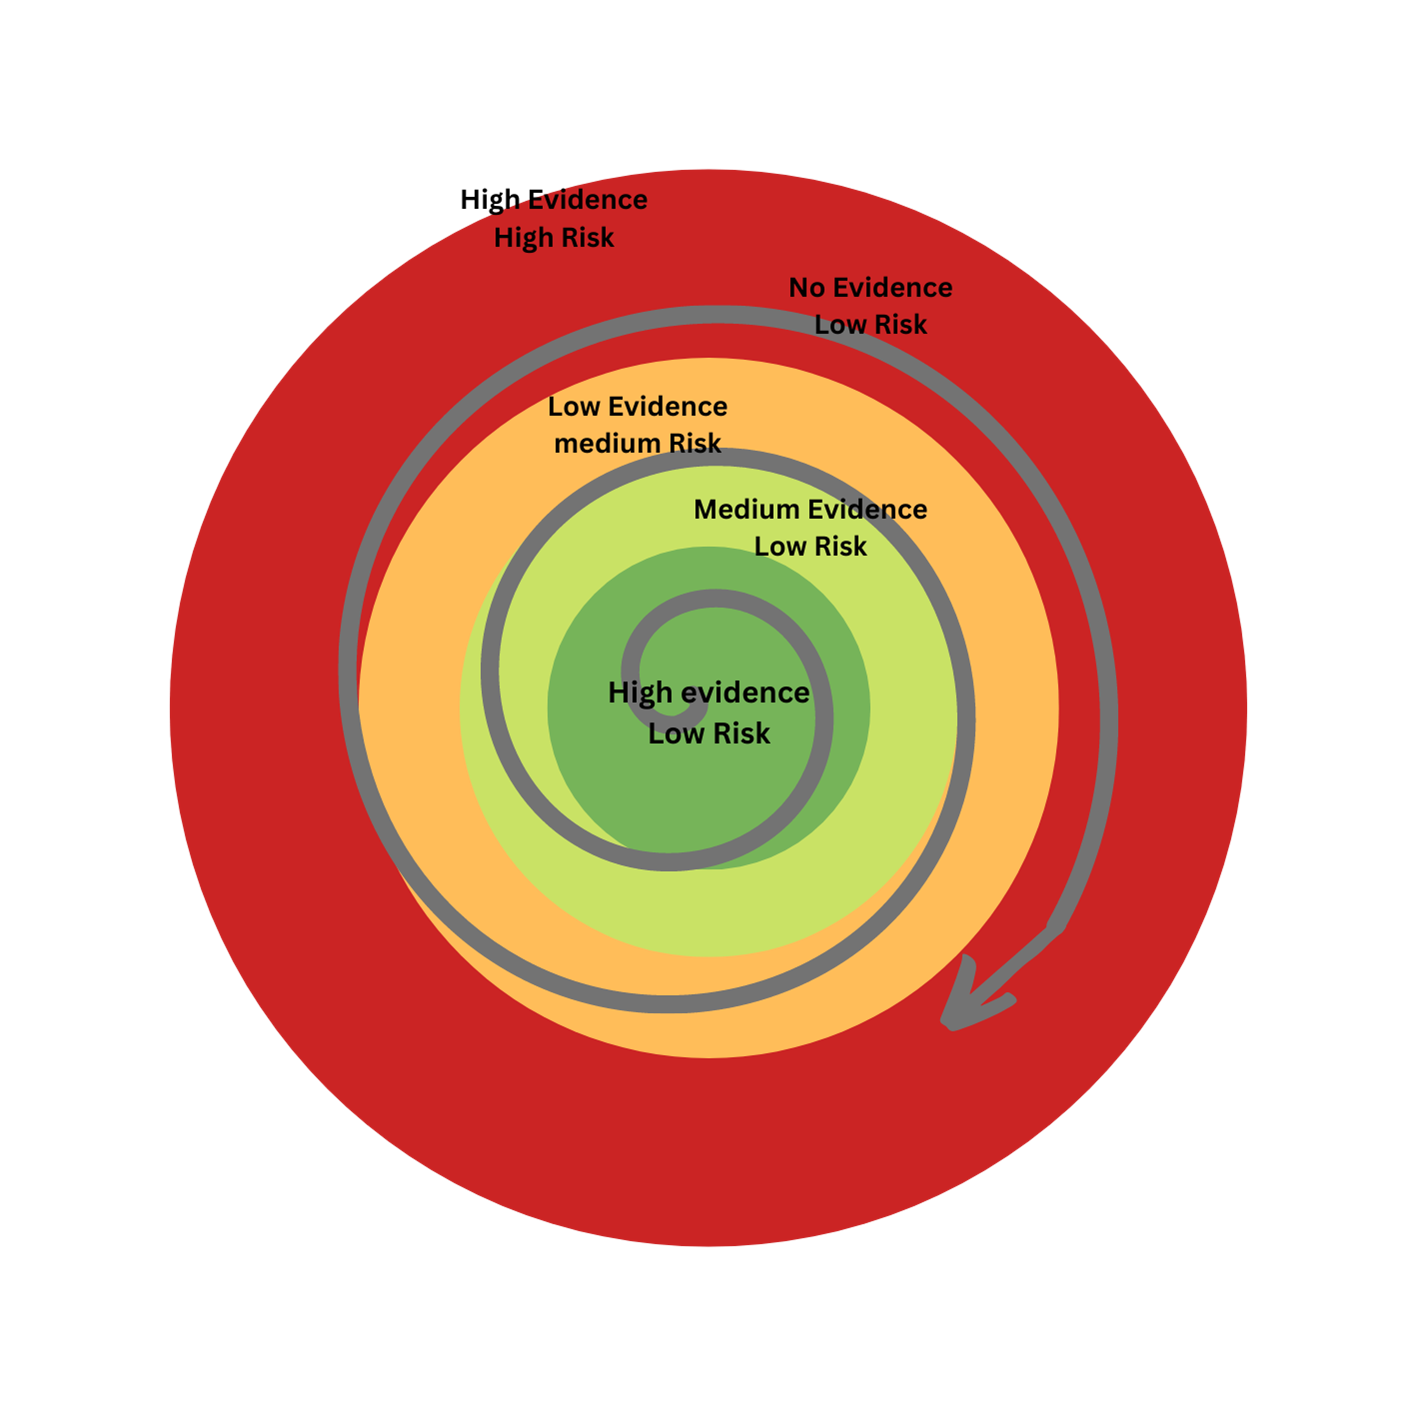
\includegraphics[width=4.16667in,height=\textheight,keepaspectratio]{images/RiskEvidence.png}

}

\caption{\label{fig-RiskEvidence}Wie wir uns im Feld der Evidenz bewegen
sollten}

\end{figure}%

\section{Was und wie viel sollten unsere Kund*innen
trainieren?}\label{was-und-wie-viel-sollten-unsere-kundinnen-trainieren}

Den ersten Anhaltspunkt für Trainingsempfehlungen bieten uns große
Organisationen oder Nationale Projekte, die sich um die Gesunderhaltung
der Bevölkerung kümmern. Die WHO Guidelines wurden zuletzt 2020 erneuert
(Bull et al., 2020). Auf nationaler Ebene setzt sich der Fond gesundes
Österreich (\url{https://fgoe.org/}) für die Durchführung der
Richtlinien ein und versorgt auch für Informationen, die leicht
verständlich und umsetzbar sind (siehe Abbildung 6).

Unsere Aufgabe als Sportwissenschafter*innen und PCs ist es, diese
Vorgaben zu propagieren und für unsere Klient*innen Möglichkeiten der
Umsetzung zu finden. Häufig konzentrieren wir uns als Trainer*innen auf
die spezifische Umsetzung von intensiven und expliziten Übungen. Jedoch
sollte vor allem \textbf{die allgemeine Aktivität bei mittlerer
Intensität} im Zentrum stehen. Diese allgemeine Aktivität ist zumindest
äquivalent (wenn nicht überlegen) in der Verringerung der Mortalität.
Dies bestätigte auch eine der größten Kohortenstudien der letzten Jahre
(Lee et al., 2022), sowie eine größere Meta-Analyse (Ekelund et al.,
2019).

Für manche sportbegeisterte PCs scheinen die vorgeschlagenen
Trainingsvolumina in den Guidelines vielleicht etwas niedrig. Es zeigt
sich jedoch, dass der gesundheitliche Haupteffekt von Training wirklich
mit den ersten \textbf{ca. 180 -- 240 Minuten} erreicht ist (Ekelund et
al., 2019). Für die Kommunikation mit Klient*innen ist dabei wichtig,
dass diese Werte keine magischen Zahlen sind. \textbf{JEDE Aktivität ist
gut}, egal wie kurz oder wie gering! (Siehe auch
\href{https://www.who.int/news/item/25-11-2020-every-move-counts-towards-better-health-says-who\#:~:text=Up\%20to\%205\%20million\%20deaths,global\%20population\%20was\%20more\%20active.}{\emph{Every
Step counts}}).

\begin{figure}

\centering{

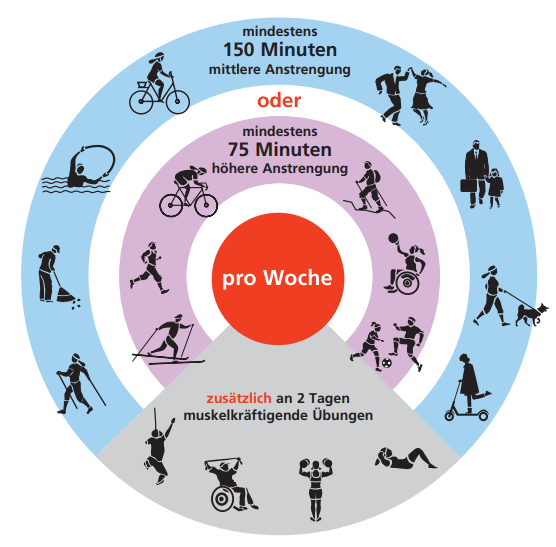
\includegraphics[width=4.16667in,height=\textheight,keepaspectratio]{images/FGO_Bewegung.png}

}

\caption{\label{fig-FGO}Fond gesundes Österreich, Zugriff 2024
https://fgoe.org/medien/Brosch\%C3\%BCren-Folder-Plakate}

\end{figure}%

Dies alles gilt vorrangig für Herzkreislauftraining. Krafttraining wird
in den Richtlinien zwar immer fokusierter angesprochen, bleibt aber
trotzdem leicht im Hintergrund. Der FGÖ gibt 2x pro Woche 30min
Krafttraining zur Gesundheitssteigerung an. Mehr ist besser? Nun, gleich
zwei aktuelle Meta-Analysen wurden zu dieser Frage im Jahr 2022
veröffentlicht. Die inkludierten Studien überscheiden sich und die
Arbeiten kamen zu sehr ähnlichen Ergebnissen (Momma et al. 2022;
Shailendra et al. 2022). Auch diese Artikel beschäftigen sich rein mit
der Sterblichkeit durch die größten, nicht übertragbaren Krankheiten
unserer Gesellschaft. In den Arbeiten wurde anhand von insgesamt 16 bzw.
10 Studien gezeigt, dass höhere Umfänge an Krafttraining nicht besser,
in manchen belangen sogar schlechter sind! Bereits mit 140-150 min
Krafttraining pro Woche annihiliert sich der positive Effekt auf die
Gesamtsterblichkeit. Höhere Umfänge sind bereits mit tendenziell
negativen Effekten verbunden Figure~\ref{fig-Momma2022}.

\begin{figure}

\centering{

\pandocbounded{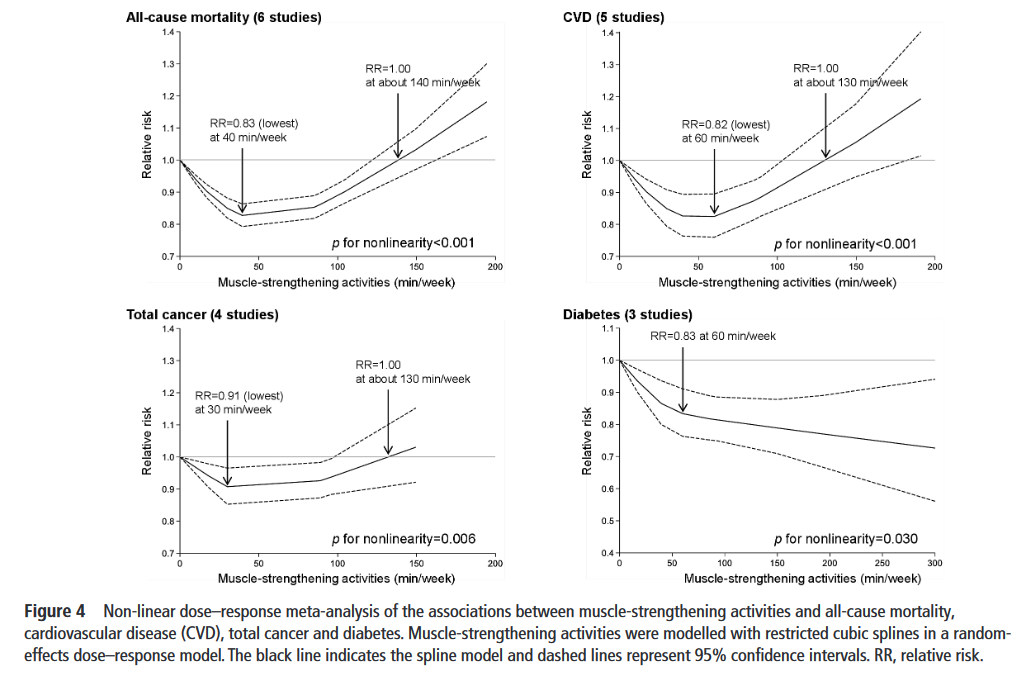
\includegraphics[keepaspectratio]{images/Momma_Risk.png}}

}

\caption{\label{fig-Momma2022}Risk-Ratio Sterblichkeit in Abhängigkeit
zu Krafttraining (Momma et al., 2022, p.~6)}

\end{figure}%

Bedacht werden sollte in jedem Fall, dass wir uns hier auf die
wichtigsten Krankheiten und Sterblichkeitsraten fokussiert haben.
Bekanntlich ist aber nicht nur wichtig \emph{wie lange} man lebt,
sondern auch \emph{wie} man lebt. Die Lebensqualität und
Selbstständigkeit im Alter ist in jedem Fall abhängig von Kraft und
Muskelfunktion. Außerdem scheint auch immer mehr Evidenz darauf zu
deuten, dass eine Kombination von Ausdauer und Kraft einen besonderen
gesamtgesundheitlichen Benefit für ältere Personen und Patient*innen zu
bietet (Fan et al. 2021; Marzolini, Oh, and Brooks 2012).

\section{Die ersten Einheiten mit Anfänger*innen -- Wie soll ich
starten?}\label{die-ersten-einheiten-mit-anfuxe4ngerinnen-wie-soll-ich-starten}

Der folgende Auszug ist vorrangig auf meiner eigenen Erfahrung aufgebaut
und bietet nur einen Anhaltspunkt. Diskussionen und Gegenmeinungen sind
wie immer im Rahmen der Lehrveranstaltung erwünscht.

\textbf{Beginne mit einer Unterbelastung:}

Ein häufiger Fehler im PC ist es, Trainierende in den ersten Stunden zu
stark zu belasten. Starker Muskelkater oder kleiner Verletzungen können
zu einem raschen Ende der Trainingskarriere führen. Dies gilt besonders
für Personen, für die es schon viel Überwindung gebraucht hat, überhaupt
ein Training zu starten. Es bietet sich also an immer der Devise zu
folgen: „You can easily do more tomorrow. But you can't undo
exercises.''

Auf der anderen Seite gibt es Klient*innen, die anfangs denken, dass nur
hartes Training ein effektives Training ist. Manche potentielle
Kund*innen konnte ich in der Vergangenheit auch dadurch nicht
überzeugen, regelmäßig meine Leistungen in Anspruch zu nehmen, weil mein
Training „zu einfach'' (= ineffektiv) war. Bei Neukunden gilt es also
früh genug zu erkennen, was ihre Erwartungen und Überzeugungen zu
Training sind. Dies bedeute nicht, dass man alle Erwartungen erfüllen
muss. Aber man sollte zumindest die unterschiedlichen Auffassungen
aufzeigen können und ein Gespräch mit den Kund*innen starten können.
Mein „Trick'' für diese letzte Kund*innen ist dann oft, sie mit einer
wenig strukturell belastenden Übung und hohen Wiederholungszahlen
subjektiv zu erschöpfen und Muskelkater eher in Körperpartien zu
erzeugen, die wenig Einfluss auf ihren Alltag haben werden (lieber Arme
oder Bauch als Oberschenkel).

\textbf{Bei Anfänger*innen funktioniert alles:}

Bei Neulingen im Training gibt es einen \textbf{großen Transfer} in der
Leistungsfähigkeit. Krafttraining verbessert die Leistung bei
Ausdauertests und umgekehrt. Dieser Transfer hält natürlich nicht lange
an und verringert sich mit zunehmender Spezialisierung und
Trainingsfortschritt. Außerdem ist zu beachten, dass dieser Transfer
vorrangig für die Funktion (Funktionelle Tests haben mehr zutragende
Komponenten) ersichtlich ist. Das bedeutet aber nicht zwangsläufig, dass
es auch zur Verbesserung derselben darunter liegenden physiologischen
Parameter kommt. Beispielsweise verbessert Krafttraining und
plyometrisches Training häufig die Leistungsfähigkeit in Lauftests.
Trotzdem verbessern sich weder Ruhepuls noch VO2max. Das gilt
wahrscheinlich für viele unterschiedliche Kohorten und wurde sowohl für
Ausdauerathlet*innen (Beattie et al. 2014) als auch Patient*innen
gezeigt (Li et al. 2020).

Die schnellsten Erfolge zeigen sich bei Anfängern tendentiell beim
Krafttraining. Natürlich sind diese Verbesserungen oft mit besserer
Technik und Ansteuerung verbunden und weniger (aber auch) mit
strukturellen Änderungen. Schnelle erfolge erhöhen bei Einsteiger*innen
die Adhärenz. Daher ist meine Empfehlung bei fast allen Neueinsteigern
mit einem Fokus auf Krafttraining zu beginnen.

\subsection{Blockperiodisierung aus Sicht des klientenzentrierten
PTs}\label{blockperiodisierung-aus-sicht-des-klientenzentrierten-pts}

Blockperiodisierung steht für fokussierte Phasen, in denen an wenigen
Qualitäten gearbeitet wird (Stone et al., 2021). Aus Sicht der PTs ist
diese Herangehensweise besonders aus psychologischer Sicht vorteilhaft.
Das klare Setzen eines Schwerpunkts für einen festgelegten Zeitraum
hilft den Trainierenden motivational. Auch das Besprechen und Darlegen
der später folgenden Blöcke kann als Ansporn genutzt werden.
Trainierende fokussieren sich für einen kurzen Zeitraum auf wenige
Inhalte. Das kann nicht nur für Training, sondern auch für Life-style
Coaching gut angewendet werden. Zum Beispiel könnte ein Prozessziel
eines Klienten mit Einschlafproblemen sein sich für die nächsten zwei
Wochen nur darauf zu beschränken, dreißig Minuten vor dem zu Bett gehen
keine Bildschirmaktivitäten mehr durchzuführen. Darauf aufbauend kann,
wie im Training auch, ein weiterer Block gebaut werden.

Da es typischerweise keinen externen Zeitpunkt gibt zu dem
Gesundheitssportler*innen die höchste Leistung bringen
müssen\footnote{Natürlich gibt es die Personen, die zu einem Zeitpunkt
  (Hochzeit, Badurlaub) ihre „Topfigur'' haben wollen. Diese sollten
  wohl mehr so behandelt werden wie klassische Bodybuilder, die auf die
  Bühne wollen.}, bietet es sich an die Blöcke nach Jahreszeiten oder
nach anderen gesellschaftlichen Gegebenheiten zu strukturieren. Im
Hochsommer (Périard, DeGroot, and Jay 2022) und im Winter (Gatterer et
al. 2021) bieten sich für die meisten Personen keine HIIT Outdoor
Trainings an. LSD sind hier noch besser geeignet (Flüssigkeitszufuhr
beachten
\href{https://www.embodymate.at/2020/08/21/wasser-1-gesundheit-und-trinkmenge/}{Blogpost}).
Höhere Intensitäten sind eher bei milderen Temperaturen zu setzen.

In den Schulferien haben Eltern, wenn sie bei den Kindern zu Hause
bleiben möchten, manchmal andere Bedürfnisse als während der Schulzeit.
So könnten in den Ferien Home-Trainingspläne mehr Sinn machen und in den
Schulzeiten Einheiten im Fitnessstudio.

Ernährungsumstellungen mit Zuckerreduktion und mehr frischem Obst und
Gemüse sind leichter im Sommer zu implementieren als kurz vor
Weihnachten. Vor Weihnachten werden sich jedoch andererseits viele
Menschen ihrem Stresslevel bewusst und hier können Strategien geplant
und umgesetzt werden
(\href{https://www.embodymate.at/2020/12/24/entspannung-erlernen/}{Entspannung
lernen}).

Bei einer Blockperiodisierung ist es nicht notwendig (und meist nicht
möglich) einen genauen Plan für kommende Zyklen auszuarbeiten. Jedoch
zeugt es von Transparenz und Struktur Klient*innen bereits im Vorhinein
die grobe Zielsetzung und Methoden der kommenden Zyklen vorzulegen.

Um die Dauer eines Trainingsblocks festzulegen gibt es drei
Grundsätzliche Strategien:

\begin{itemize}
\tightlist
\item
  Absolute Zeitbasiert (z.B. 8-12 Wochen)
\item
  Relative Zeitbasiert (z.B. für 12 Trainingseinheiten)
\item
  Absolut Zielbasiert (z.B. wenn X nach Kriterium Y erfüllt wurde)
\end{itemize}

Keine der Strategien ist den anderen absolut überlegen. Wo siehst du die
Vor- und Nachteile der Strategien?

\begin{tcolorbox}[enhanced jigsaw, colback=white, toptitle=1mm, opacitybacktitle=0.6, title=\textcolor{quarto-callout-note-color}{\faInfo}\hspace{0.5em}{Note}, colframe=quarto-callout-note-color-frame, colbacktitle=quarto-callout-note-color!10!white, toprule=.15mm, rightrule=.15mm, bottomtitle=1mm, left=2mm, arc=.35mm, opacityback=0, titlerule=0mm, coltitle=black, breakable, leftrule=.75mm, bottomrule=.15mm]

Einschub Individualität -- Biologische Faktoren:

Vielleicht fallen dir bei den Stichworten biologische Rhythmen und
Zyklen noch weitere praktische Überlegungen der Trainingsinhalte ein.
Zyklusorientiertes Training für Frauen ist zum Beispiel aktuell wieder
im Trend. Frauen durchlaufen innerhalb des Menstruationszyklus
hormonelle Schwankungen, welche theoretisch zu unterschiedlicher
Anpassungsfähigkeit, Trainingsleistung, Verletzungsanfälligkeit und
psychologischer Resilienz führen (Kudielka and Kirschbaum 2005; Reed and
Carr 2000; Sims and Heather 2018). Leider gibt es noch immer eine starke
Unterrepräsentation weiblicher Probandinnen in Exercise Science (Cowley
et al. 2021). Während wir eindeutige physiologische Unterschiede
identifizieren können (z.B. in den wichtigsten anabolen Hormonen),
wissen wir im Allgemeinen nicht genau, ob und wie wir in der
Trainingsplanung darauf eingehen müssen (B. Roberts, Nuckols, and
Krieger 2020). Hinzu kommt eine Bandbreite an hormonellen Kontrazeptiva,
die weit verbreitet sind. Leider gibt es jedoch kaum Studien in der
Exercise Science zu diesen unterschiedlichen Typen. Fast ausschließlich
werden orale Kontrazeptiva (v.a. der zweiten Generation) erforscht
(Carmichael et al. 2021). Wie gehen wir also mit solchen Unsicherheiten
in der Praxis um?

\end{tcolorbox}

Abschließend soll eine Kurzfassung der Programming Considerations nach
Stone und Kollegen (2021), welche auch für PTs wichtig sein könnte,
dargestellt werden:

\begin{itemize}
\tightlist
\item
  Multi-Joint Übungen verwenden
\item
  Die wichtigsten Übungen zuerst
\item
  Kraft vor Ausdauer am jeweiligen Trainingstag
\item
  HIIT anstelle von LSD mit Kraft kombinieren, um Interferenzen zu
  minimieren
\item
  Wave-Loading bei mehreren Einheiten pro Wochen
\end{itemize}

Jedoch wirst du dich an Kapitel 6 und 7 erinnern und erkennen, dass
diese Prinzipien/Modelle des Programmings ebenfalls angepasst werden
können und keiner absoluten Wahrheit für Personal Coaching und
Gesundheitssport entsprechen.

\section{Warm-up}\label{sec-warm-up}

Das Aufwärmprogramm soll den Trainierenden auf die Einheit vorbereiten
und spezifisch auf die Inhalte des Hauptteils ausgelegt sein. Im PC wird
das Warm-up zumeist nach einem kurzen Check-in und generellen Austausch
(Tagesverfassung des Trainierenden, Rückblick auf vergangene Tage,
Ausblick auf die heutige Trainingseinheit, etc.) durchgeführt. Die
Zielsetzung des Warm-up ist es, die Leistung in der Einheit zu erhöhen
und das Verletzungsrisiko zu verringern. Während ersteres durch ein gut
durchgeführtes Warm-up gut zu erreichen ist, scheint es nach aktueller
Forschunglage unklar inwieweit das Verletzungsrisiko gesenkt werden
kann. Je nach Verletzung und Sportart existiert nur eine begrenzte Menge
an Literatur, die zusammengefasst aber auf einen positiven Effekt
hinweist(McCrary, Ackermann, and Halaki 2015; Behm et al. 2023). Zur
Vermeidung und Verbesserung mancher Überlastungserscheinungen, ist ein
gutes Warm-up jedoch unumgänglich. Tendinopathien zeigen zum Beispiel
eine starke, akute Verbesserung durch Aufwärmen, wodurch effektives (und
notwendiges) Training erst möglich wird {[}{``How to {Self-Manage
Achilles Tendon Pain} and {When} to {See} a {Health Professional}''}
(2024); de Vos et al. (2021); {]}. Auch Personen mit Arthrose reagieren
zumeist recht sensibel auf Belastung ohne vorhergehenden langsamen
Aufbau der Belastung. Gesunde, junge Personen sind im allgemeinen
weniger auf das Aufärmen angewiesen als ältere Personen. Aus Sicht
akuter Leistungsverbesserung sollte noch erwähnt werden, dass gerade
hochtrainierte Personen von einem umfangreichen Aufwärmen profitieren,
während weniger trainierte (aber gesunde) Personen mit kürzeren
Aufwärmprozessen auskommen.

\subsection{RAMP}\label{ramp}

Ian Jeffreys schlägt das \textbf{RAMP-Protokoll} als Guideline vor. RAMP
steht für \emph{Raise}, \emph{Activate}, \emph{Mobilize} und
\emph{Potentiate} und soll die effktiven Phasen eines Aufwärmprogramms
für sportliche Betätigung darstellen (Jeffreys 2007; Jeffreys in Hough
and Schoenfeld 2021). \emph{Raise} steht für das Erhöhen der
Körperkerntemperatur (+3-4°C) und wird zumeist durch aktive Maßnahmen
erreicht. Kontinuierliche, low-impact Inhalte eignen sich hier zumeist
gut. \emph{Activate} steht für die Ativierung der spezfischen
Körperregionen, die für das Training gebraucht werden. Hier können
low-load Übung für die wichtigsten Muskelgruppen eingesetzt werden. Für
Personen mit einer Verletzungsvergangenheit im Schutlergurt könnten zum
Beispiel Übungen für die Rotatorenmanschette eingesetzt werden.
\emph{Mobilize} steht für die Mobilisierung der Gelenke. Statische oder
dynamische Beweglichkeitsübungen sind das Mittel der Wahl. Dynamischen
Übungen sollten der Vorzug gegeben werden. Häufig wird aufgrund des
mehrfach nachgewiesenen ``stretch-induced performance loss'' gegen
statisches Dehnen argumentiert. Dieser Effekt ist jedoch recht gering
und kann vorrangig beobachtet werden, wenn Dehnpositionen lange gehalten
werden (\textgreater60s) und kein weiteres Warm-up durchgeführt wird
(Behm et al. 2021). Dynamisches Dehnen erhöht die Herzfrequenz und den
Blutfluss in der Muskulatur mehr als passives Dehnen. Dynamische
Beweglichkeitsübungen bieten darüber hinaus mögliche(!) Vorteile der
chronischen Anpassung im Bereich des Leistungsfähigkeit,
Bewegungsqualität Koordination und Muskel-Sehnen Morphologie (Behm et
al. 2023). Damit sollte statisches Dehnen in den meisten Fällen an das
Ende des Trainings (siehe Cool-down) oder in eine eigene Einheit verlegt
werden. \emph{Potentiate} steht für die Aktivierung der Trainierenden
aus neuromuskulärer und auch mentaler sicht. Hier wird meist vom ``Post
activation performance enhancement effect'' (kurz PAP oder besser PAPE /
treppe effect) gesprochen (Blazevich and Babault 2019). Durch den PAPE
Effekt erhöht sich die Leistungsfähigkeit sich nach kurzer, nicht
ermüdender Aktivität hoher Intensität (\textgreater80\%). Hierfür können
plyometrische und explosive Bewegungen wie Sprints, Würfe/Stöße oder
Sprünge zur Anwendung kommen. Aber auch kurze isometrische Übungen mit
hoher Intensität könnten sich aufgrund ihrer geringen Verletzungsgefahr
und Belastung der Gelenke gut anbieten (Finlay et al. 2022; Seitz and
Haff 2016b).

Im Personal Coaching lässt sich das Warm-up mit zwei weitgehend
unterschiedlichen Ansätzen durchführen. Es kann als Teil der 1-on-1
Betreuung innerhalb der betreuten Einheit durchgeführt werden oder
Klient*innen führen das Warm-up bereits vorher eigenständig druch.

\subsection{Warm-up als Möglichkeit der Bewegungsvielfalt und
Koordinativen
Schulung}\label{warm-up-als-muxf6glichkeit-der-bewegungsvielfalt-und-koordinativen-schulung}

Das Warm-up kann nicht nur als Notwendigkeit angsehen werden, um das die
vorliegende Trainingseinheit effektiver oder sicherer zu machen. Es kann
auch als Chance wahrgenommen werden, langfristig Verbesserungen zu
erzielen und Kompetenzen der Trainierenden zu fördern. Das Warm-up soll
also bereits chronische Anpassungen erzielen. Diese sind möglicherweise
weniger physiologischer als vielmehr technisch-koordinativer Natur, da
die Belastung notgedrungen geringer sein muss. Es werden bereits Übungen
eingesetzt, die wichtig für die Bewegungsfähigkeiten der Klient*innen
sind. Für Läufer*innen könnten das zum Beispiel koordinative Laufübungen
sein. Besonders gut lässt sich diese Herangehensweise mit der dirkten
Betreuung im 1-on-1 Setting kombinieren. Die Trainierenden werden also
bereits während dem Aufwärmen direkt von den PCs betreut. Es bietet sich
in diesem Zusammenhang auch an, ein sehr variantenreiches Aufwärmen zu
gestalten. Der Hauptteil des Trainings wird zumeist relativ fix im
Trainingsplan festgelegt. Das Warm-up kann damit etwas Abwechslung
bieten und gleichzeitig die Bewegungsvielfalt und verschiedene
koordinative Fähigkeiten und Fertigkeiten schulen.

\subsection{Warm-up als Möglichkeit Eigenständigkeit im Training zu
üben}\label{warm-up-als-muxf6glichkeit-eigenstuxe4ndigkeit-im-training-zu-uxfcben}

Ein anderer Zugang im Personal Coaching ist, Klient*innen auch in der
1-on-1 Betreuung selbstständig aufwärmen zu lassen. Dies verschafft Zeit
während dem Hauptteil und kann so zu einer effektiveren Betreuung
beitragen. In der Praxis sollten Kient*innen langsam an die
vollständigen Eigentsändigkeit hingeführt werden. Die Trainierenden
könnten also zu Anfangs vollkommen strukturiert und überwacht eine
Warm-up Routine durchführen. Die direkte Überwachung wird schließlich
schrittweise abgebaut (z.B. alle paar Wochen ein gemeinsames Aufwärmen)
wobei die Entscheidungsfreiheit der Klient*innen stetig zunimmt. Der
trainierenden Person kann schrittweise das RAMP Protokoll (oder ein
anderes System) beigebracht werden. Wenn am Anfang zum Beispiel der
Radergometer zur Erhöhung der Herzfrequenz (\emph{Raise}) eingesetzt
wird, könnte später Freiheit über die Bewegungsmodalität gegeben werden.
Wobei trotzdem Vorgaben der Belastungsdauer und Intensität durch die PCs
stattfinden.

\section{Weiterführende Literatur:}\label{weiterfuxfchrende-literatur-1}

M. Jovancović -- Strength Training Manual Volume 1 und 2 bieten einen
alternativen Ansatz zu „traditionellen'' top down
Trainingsplanungsmodellen. Die Bücher beschäftigen sich vorrangig mit
S\&C im Sportbereich. Besonders die Philosophie dahinter (Volume 1)
bietet sich jedoch auch für Personal Coaches an.

Stone et al.~2021 konstruieren Argumente für die Block Periodisierung im
Krafttraining. Die Autoren sind teilweise seit Jahrzehnten Forscher und
Verfechter von Periodisierung. Ihre Argumente sollten nicht ganz über
den Haufen geworfen werden.

\section{Literatur}\label{literatur-10}

\bookmarksetup{startatroot}

\chapter{Selbststudiumsaufgaben -
SSA}\label{selbststudiumsaufgaben---ssa}

\begin{verbatim}
systemfonts and textshaping have been compiled with different versions of Freetype. Because of this, textshaping will not use the font cache provided by systemfonts
\end{verbatim}

Die SSAs erscheinen wöchentlich im Moodle Kurs zum Seminar. Beachte,
dass es unterschiedliche Kriterien zum Erfüllen der Aufgaben gibt. Für
machen reicht es, wenn du ein kurzes ``ok'' im Antwortenfeld
hinterlässt. Dies ist vor allem dann der Fall, wenn die Antworten
potentiell persönliche Informationen von dir oder deinen Klient*innen
beinhalten könnten. Bei anderen Aufgaben musst du eine Datei hochladen
oder kurze Antworten (stichwortartig) hinterlassen.

\section{Organisation}\label{organisation}

\subsection{Semesterplan}\label{semesterplan}

\textbf{Start:} Erste Einheit\\
\textbf{Dauer:} 2 Wochen\\
(Aufgrund der Möglichkeit, dass Studierende erste in der zweiten Einheit
eingeschrieben werden können.)

\textbf{Beschreibung:}\\
Verschaffe dir Überblick im Skript und auf Moodle. Plane das Semester!

\textbf{Aufgabe:}\\
``Planen ist alles, ein Plan ist nichts!'' - Eisenhower

Organisiert zu sein und vorausschauend zu planen, ist eine der
wichtigsten Kompetenzen als Coach. Klient*innen verlassen sich auf deine
zeitnahe und voraussehnede Bearbeitung ihrer Anliegen. Vorbereitet zu
sein, ist außerdem ein erlernbarer und machbarer \emph{Skill}. Deine
ersten Aufgaben beziehen sich gleich darauf:

\begin{enumerate}
\def\labelenumi{\arabic{enumi})}
\tightlist
\item
  Lies die Einleitung im Skriptum (Chapter~\ref{sec-einleitung}). Hier
  findest du alle Informationen zum Ablauf der LV.
\item
  Schreibe dir auf was unklar ist. Besprich es mit Kolleg*innen und
  bring offene Fragen zur nächsten Einheit.
\item
  Zücke deinen Kalender versichere dich, dass du bei allen Terminen
  (voraussichtlich) Zeit hast. Sprich geplante Abwesenheiten direkt in
  der nächsten Einheit an.
\end{enumerate}

Als abgeschlossen gilt diese Aufgabe, wenn du ein ``OK'' in das Textfeld
schreibst.

\subsection{Schaffe dir Platz im
Kalender}\label{schaffe-dir-platz-im-kalender}

\textbf{Start:} Erste Einheit\\
\textbf{Dauer:} 2 Wochen\\
(Aufgrund der Möglichkeit, dass Studierende erste in der zweiten Einheit
eingeschrieben werden können.)

\textbf{Beschreibung}\\
Plane fixe Zeitfenster in denen du dich mit dem Seminar beschäftigst.

\textbf{Aufgabe}\\
Dieses Seminar hat 2 ECTS (= 50 - 60h) und etwas mehr als die Hälfte
dieser Zeit (\textasciitilde{} 30h) wirst du NICHT in den
Präsenzeinheiten (20 - 22h) aufwenden (siehe
Chapter~\ref{sec-einleitung}).

Von Semester Anfang bis vorlestungsfreie Zeit sind es ca. 15-16 Wochen.
Das ergibt für die 30 Arbeitsstunden ca. 2h Arbeit pro Woche.

Du hast wöchentliche kurze Aufgaben (wie diese hier). Plane für die
kommenden \textbf{4 Wochen} jeweils zwei Blöck von \textbf{30-60min} pro
Woche für die Erfüllung dieser SSAs, sowie Planung und Dokumentation der
Personal Coachings. Trage sie \textbf{jetzt} in deinen Kalender ein.

Versuche realistische Zeitfenster zu planen, die du auch wirklich
einhalten kannst.

Anschließend hast du 4 Wochen Zeit, dich zu üben konsistent zu sein.
Denke daran, dass eine ähnliche Situation auf deine Klient*innen
zukommen kann. Sie ``sollen'' einen Trainingsplan einhalten. Nicht immer
ist das zu schaffen und es kommen verschiedene Herausforderungen zum
Vorschein, die sie an den Trainingseinheiten hindern. Es bedarf Übung,
sich an einen Plan zu halten. Jedes mal, wenn du es schaffst wird es
etwas einfacher. Wie im Training gilt:

\textbf{Consistence is Queen!}

\section{Berufsethik und Berufsbild}\label{berufsethik-und-berufsbild}

\subsection{Angebotsrecherche}\label{angebotsrecherche}

\textbf{Start:} Woche 2\\
\textbf{Dauer:} 1 Woche

\textbf{Beschreibung}\\
Du findest Informationen zum Beruf des Personal Coach oder Personal
Trainer*in im Kapitel Was ist Personal Coaching
(Chapter~\ref{sec-was-ist-personal-coaching}).

Was bieten Personal Trainer*innen rund um Wien oder in anderen Gegenden?

\textbf{Aufgabe}\\
Schaue dir unterschiedliche Web-Auftritte von Personal Trainer*innen an.
Du kannst Webseiten und Social Media einsetzen.

Welche Angebote gibt es? Welche Marketingstrategien werden eingesetzt?
Welche Zielgruppen werden angesprochen? Wie sind Trainer*innen
ausgebildet? In welchem Arbeitssetting arbeiten sie (Hometraining,
online, Studio, \ldots) Was fällt dir sonst ein?

Trage stichwortartig deine Erkenntnisse zusammen und bringe sie als
Diskussionsmaterial zur nächsten Einheit.

\subsection{Was macht gute PCs aus?}\label{was-macht-gute-pcs-aus}

\textbf{Start} Woche 2\\
\textbf{Dauer} 1 Woche

\textbf{Beschreibung:}\\
Du findest Informationen zum Beruf des Personal Coach oder Personal
Trainer*in im Kapitel Was ist Personal Coaching
(Chapter~\ref{sec-was-ist-personal-coaching}). Lies dir das Kapitel
durch. Anschließend sprich mit potentiellen Klient*innen von Coaches.

\textbf{Aufgabe:}\\
Bearbeite im im Laufe der Woche diese Aufgaben und beschreibe im
Antwortfeld kurz deine Erkenntnisse.

Sprich mit mindestens drei Personen aus deinem Umfeld. Wähle dazu, wenn
möglich sehr unterschiedliche Personen aus (Alter, Geschlecht,
Trainingserfahrung, Gesundheitszustand\ldots). Frage sie, was sie von
Personal Training halten und was sie sich von den Coaches erwarten
würden. Was wäre ihnen wichtig? Sammle die Antworten als Stichworte.
Dann setze dich hin und mache dir ein paar Minuten selbst dazu Gedanken.
Was sind wichtige Eigenschaften und Kompetenzen von Trainer*innen?
Schreibe deine Ergebnisse in Stichworten auf.

\section{Erstelle eine Berufsethik}\label{erstelle-eine-berufsethik}

\textbf{Start:} Woche 2\\
\textbf{Dauer:} 2 Wochen

\textbf{Beschreibung}\\
\textbf{Eine Berufsethik schützt!} Du findest Informationen zur Ethik im
Kapitel Berufsethik und Berufsbild (Chapter~\ref{sec-berufsethik}).
Erstelle in dieser SSA deine eigene Berufsethik.

\textbf{Aufgabe:}\\
Lies die vorgeschlagenen ethischen Grundlagen der verschiedenen
Berufsgruppen und überlege dir, wie ein ähnliches Dokument für PCs
aussehen könnte. Was wären die für dich wichtigsten Punkte, die du in
einer solchen Berufsethik sehen möchtest? Beschreibe im Antwortfeld
deine wichtigsten Punkte der Berufsethik für Personal Coaches.

\section{Ziele setzen}\label{ziele-setzen-1}

\subsection{Deine Ziele}\label{deine-ziele}

\textbf{Start:} Woche 3\\
\textbf{Dauer:} 1 Woche

\textbf{Beschreibung}\\
Genauso wichtig wie die Ziele deiner Klient*innen, sind deine Ziele.
Werde dir deiner Ziele bewusst! Für diese Aufgabe brauchst du ein bis
zwei Blatt Papier, einen Stift (analog ist wirklich besser) und 20-30min
ungestörte Zeit.

\textbf{Aufgabe:}\\
Es gibt viele verschiedene Zielsetzungsübungen. Eine, die auf der
Zuschreibung deiner Werte basiert, haben wir wahrscheinlich in der LV
ausprobiert. Hier ist eine andere. Geh mit frischer Neugierde hinein -
\emph{Shoshin}

Nimm dir deinen Zettel und Stift zur Hand, um die Punkte der Reihe nach
zu bearbeiten. Schließe am Ende die Aufgabe ab indem du ein ``OK'' oder
eine sonstige Anmerkung in das Textfeld schreibst. Deine persönlichen
Ziele musst du hier nicht mitteilen!

\begin{enumerate}
\def\labelenumi{\arabic{enumi}.}
\item
  \textbf{Quo Vadis?} Welche Ziele in Bezug auf Bewegung Gesundheit oder
  Training hast du? Alles was dir einfällt. Frei aus dem Bauch heraus
  und stichwortartig.
\item
  \textbf{Via Negativa!} Schaue dir deine Ziele an und setze
  Prioritäten. Schaffst du es zumindest die Hälfte der Ziele zu
  streichen? Was bleibt übrig, das dir wirklich im Moment am Herzen
  liegt? Je mehr du streichst, desto mehr Fokus und Erfolg bleibt übrig!
  Schreibe die übrigen gebliebenen Ziele, noch einmal auf ein neues
  Blatt Papier. Was machst du mit den anderen Ziele, die du davor
  gestrichen hast? Diese sind auch wichtig! Denn diese zu verfolgen gilt
  es dringend zu vermeiden! Bewahre dir also den Zettel mit den
  gestrichenen Zielen ebenfalls auf.
\item
  \textbf{Affektbilanz!} (Storch \& Tschacher, 2016) Schau dir jedes
  dieser wichtigen Ziele einzeln an und bewerte auf zwei Skalen:

  \begin{enumerate}
  \def\labelenumii{\arabic{enumii}.}
  \setcounter{enumii}{2}
  \tightlist
  \item
    Löst dieses Ziel und die Arbeit an diesem Ziel etwas Positives in
    dir aus? Auf einer Skala von 0-100, wie positiv sind deine
    Emotionen, wenn du an das Ziel denkst.
  \item
    Löst dieses Ziel und die Arbeit an diesem Ziel gleichzeitig etwas
    Negatives in dir aus? Auf einer Skala von 0-100, wie negativ sind
    deine Emotionen, wenn du an das Ziel denkst.
  \end{enumerate}

  Verwende dazu den Affektregler für jedes einzelne Ziel. Wichtig ist,
  dass du dir dabei etwas Zeit lässt und dir das Erreichen der Ziele und
  die Arbeit an den Zielen so körperlich wie möglich vorstellst.

  \begin{figure}

  \centering{

  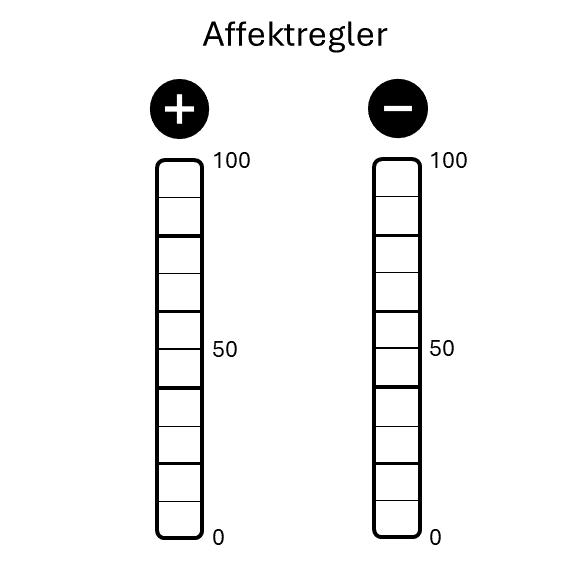
\includegraphics[width=4.16667in,height=\textheight,keepaspectratio]{Appendix/Affektregler.png}

  }

  \caption{\label{fig-affekt}Affektregler}

  \end{figure}%
\item
  \textbf{Objective!} Gibt es eine übergeordnetes Thema für deine Ziele?
  Versuche eine Art Überschrift zu finden. Ein Titel soll kurz und
  knackig sein. Gestalte ihn wie einen Leitspruch, Werbeslogan oder
  einen Buchtitel. Formuliere ihn positiv! (Beispiel: ``Training als
  Stütze''; ``Mein Weg zum ersten Halbmarathon''; ``Ausgeglichen und
  Effektiv'')
\item
  \textbf{Die 5-Minuten Aktion!} Was kannst du heute tun, um deinem Ziel
  ein kleines Stück näher zu kommen? Versuche eine Aktion zu setzen, die
  maximal 5 Minuten in Anspruch nimmt und die Kugel ins rollen bringt.
  Reflexion und planen sind gut, aber Aktion bringt Wandel!
\item
  \textbf{Hilfe Ansuchen!} Wen kannst du um Hilfe bitten? (Freund,
  Familie, Kollegen Lehrbeauftragte, \ldots) Überlege dir auch wie dir
  diese Person konkret helfen kann und bitte Sie genau darum.
\end{enumerate}

Diese Aufgabe bestätigst du mit ``ok''.

\section{Ananmese und Erstkontakt}\label{ananmese-und-erstkontakt}

\subsection{Erstelle einen
Anamnesebogen}\label{erstelle-einen-anamnesebogen}

\textbf{Start} Woche 4\\
\textbf{Dauer} 2 Wochen

\textbf{Beschreibung:}\\
Erstelle einen Anamnesebogen. Verwende ein eigenes Design, das
übersichtlich und professionell wirkt.

\textbf{Aufgabe:}\\
Überlege dir, wie du deinen Anamnesebogen einsetzen möchtest.
Verbreitete Ansätze sind:

\begin{itemize}
\item
  Die Klient*innen füllen diesen im Vorhinein alleine aus und ihr
  besprecht dann die Antworten gemeinsam. So haben sie Zeit sich
  Gedanken zu machen. Wenn du den ausgefüllten Bogen schon im Vorhinein
  zurück bekommst, kannst auch du dich besser vorbereiten. Bitte
  beachte, dass der Anamnesebogen sensible persönliche Daten enthält.
  Daher sollte er über ein sicheres Medium an dich gesendet werden.
\item
  Du füllst den Fragebogen in einem gemeinsame Gespräch vollständig aus.
  Dies hat den Vorteil, dass die Klient*innen nicht vorher schon etwas
  erarbeiten müssen. Für viele ist das Ausfüllen der Daten (womöglich
  bevor sie dich persönlich kennen) eine unangenehme Hürde. Im
  gemeinsamen Gespräch kannst du außerdem tiefere Einblicke sammeln als
  es vielleicht durch den strukturierten Bogen alleine möglich ist.
  Klient*innen sprechen selbstständig für sie wichtige Themen an und
  auch du hast mehr Freiheit.
\item
  Du lässt nur die wichtigsten Punkte (medizinisches Risk-Assessment und
  Kontaktdaten) von den Klient*innen ausfüllen, startest in ein Training
  und füllst im Laufe des Coaching Prozesses mehr und mehr aus, um es
  dann erneut aufzugreifen und mit den Klient*innen abzusprechen. Dies
  bietet den schnellsten Einstieg in das, was den meisten Klient*innen
  wichtig ist - das eigentliche Training. Es bedarf jedoch mehr Struktur
  von deiner Seite, da dir wichtige Informationen vielleicht noch fehlen
  und du diese im Nachhinein erfragen und eintragen musst.
\end{itemize}

Gib deinen fertigen Anamnesebogen unten als PDF oder Word-Datei ab und
kommentiere, wie du den Bogen einsetzen möchtest.

\subsection{Plan Update}\label{plan-update}

\textbf{Start:} Woche 4\\
\textbf{Dauer:} 1 Woche

\textbf{Beschreibung:}\\
Als Coach hältst du den Raum für Veränderungen. Du lädst zu
Veränderungen ein, planst die Schritte und kontrollierst den Erfolg. Im
Anschluss Evaluierst du die Handlungen und Ergebnisse, um so die
weiteren Schritte zu setzen.

In diese Übung wirst du deinen persönlichen Semesterplan updaten.

\textbf{Aufgabe:}\\
Vor 4 Wochen hast du dir einen Plan erstellt, der dich durch das
Semester führt. Du hast dir damals wöchentliche Zeitfenster zur
Bearbeitung der Aufgaben in deinen Kalender eingetragen.

Seither hast du neue Informationen gesammelt. Setze deinen Coaching-Hut
auf und gehe die letzten Wochen gedanklich durch.

Hat deine Herangehensweise geklappt? Mit welchen Aspekten bist zu
zufrieden? Wo solltest du nachjustieren? Du hast dich auch mit deinen
persönlichen Zielen auseinandergesetzt. Beziehe diese ebenfalls mit ein
und erstelle einen verbesserten Plan für die nächsten 4 Wochen. Du
kannst dir wieder Zeitfenster in deinen Kalender eintragen oder eine
andere Strategie überlegen. Dieses mal kannst du dir auch Gedanken dazu
machen, wie du den Erfolg deiner Strategien messbar machen kannst. Ein
``OK'' bestätigt, dass du die Aufgabe durchgeführt hast.

\section{Volition und Verhalten}\label{volition-und-verhalten}

\textbf{The goal is to keep the goal the goal!}\\
- Dan John

Motive, Ziele, eine klare Strategie und ein System sind die Zutaten für
den Erfolg. Du hast dich bereits etwas mit den Zielen beschäftigt. Nun
ist es an der Zeit, dir Strategien zurecht zulegen. Bearbeite in dieser
Woche Handlungspläne und Bewältigungspläne.

\subsection{Konkrete Pläne}\label{konkrete-pluxe4ne}

\textbf{Start:} Woche 5\\
\textbf{Dauer:} 2 Wochen

\textbf{Beschreibung:}\\
Du findest in Skript einen kurzen Abschnitt zu Handlungsplänen und
Bewältigungsplänen (Section~\ref{sec-ziel-handlung}).

\textbf{Aufgabe:}\\
Deine Klient*in und du entscheiden sich für grobe Strategien, um Ziele
zu erreichen. Die Klient*in könnte zum Beispiel einen dieser Sätze
sagen:

\begin{itemize}
\tightlist
\item
  ``Ich \emph{will} weniger Fleisch essen.''
\item
  ``Ich \emph{muss} früher ins Bett gehen.''
\item
  ``Ich \emph{sollte} im Büro die Treppen nehmen anstelle des Aufzugs.''
\item
  ``Ich \emph{darf} abends vor dem zu Bett gehen Instagram nicht mehr
  öffnen.''
\item
  ``Ich \emph{will} meinen Bizeps aufblasen.''\footnote{Beachte auch die
    Modalverben, die hierbei verwendet werden können. In der Einheit zu
    Motivation werden wir diese im \textbf{Change Talk} (Motivational
    Interviewing) wieder finden.}
\end{itemize}

Ob diese ``gute'' oder ``schlechte'' Strategien sind sei fürs Erste
dahingestellt. Um die Strategie der Klient*in zu unterstützen, wäre es
jedenfalls hilfreich einen konkreten \textbf{Handlungsplan} zu
erstellen. Welche Handlungspläne kannst du für jeden dieser Punkte
finden? Wie könnte die Klient*in jeden Satz als Handlungsplan
formulieren? Schreib diese ins Antwortfeld.

\textbf{Prepare to fail!} Manche Klient*innen wollen es nicht hören
(vielleicht willst auch du es auch nicht hören), aber es wird definitiv
Zeiten geben in denen das System nicht funktioniert und wir unserer
Handlungspläne nicht einhalten können/wollen.

Diese Situationen sollten wir antizipieren und einen
\textbf{Bewältigungsplan} dafür errichten.

Finde Bewältigungspläne für jeden der oben genannten Sätze und schreibe
sie ins Antwortfeld auf Moodle.

\section{Autonomie im Training}\label{autonomie-im-training}

Einerseits wollen deine Klient*innen, dass du deine Kompetenzen
einsetzt, um ihnen den ``perfekten'' Trainingsplan und die ``optimalen
Lösungen'' für ihre Ziele vorzulegen. Andererseits wollen sie und du,
dass sie selbstständig in ihrem Gesundheits- und Bewegungsverhalten
werden.

Werden Menschen selbstständiger und erfahren mehr über sich und ihr
Verhalten, bleiben sie auch aufmerksam und sind leichter zu coachen.

Einige Studien unterstützen die Hypothese, dass Autonomie allgemein zu
höherer Motivation und Erfolg führt. Es sollte also immer euer Ziel
sein, eure Klient*innen so autonom zu machen, wie es gerade im Moment
möglich ist. Manche sind unsicherer im Umgang mit Training, andere musst
du etwas bremsen. Allgemein gilt jedoch - gib ihnen Kompetenzen und
lasse sie mitbestimmen!

Lies im Kapitel Trainingsplanung (Chapter~\ref{sec-trainingsplanung}) im
Skript.

\subsection{Minimal Effektiver Plan}\label{minimal-effektiver-plan}

\textbf{Start:} Woche 6\\
\textbf{Dauer:} 2 Wochen

\textbf{Beschreibung:}\\
Wir wollen oft den ``perfekten Plan'' ausarbeiten und haben hohe
Ansprüche an Volumen und Intensität, das wir investieren möchten.
Zumeist ist das aber nicht möglich und auch nicht zielführend. In dieser
Aufgabe versuchst du genau den gegenteiligen Weg zu gehen. Was denkst
du, dass die eine wichtigste Komponente ist, die deine Klient*in
durchführen muss, damit der Coaching-Prozess erfolgreich ist?

\textbf{Aufgabe:}\\
Beginne bei einem Gedankenexperiment. Beschreibe die EINE Strategie, die
du denkst, dass deine Klient*innen machen sollten. Sprich dann im
Anschluss mit ihnen und versuche herauszufinden, was sie dazu denken. Wo
können sie sich vorstellen zu starten? Was denken sie, dass die eine
wichtigste Komponente ist? Spiele dabei mit ihnen das
\textbf{Gedankenexperiment}: ``Wenn wir nur eine Sache machen könnten -
was wäre es?'' Setzt dann das Experiment in die Tat um und schreibt
einen ``\textbf{Minimal-effektiven Plan}'' (MEP). Bedenke aber, dass der
MEP auch machbar und erstrebenswert (/lustvoll) für die
Klient\emph{innen sein sollte! Diesen MEP kannst du natürlich in
unterschiedlicher Weise} framen\emph{. Er kann die Basis und alles
andere ist nur das Topping oder du beschreibst diesen Plan als Backup
oder Joker. Diesen Joker können sie einsetzen, wenn sie nicht dazu
kommen ein ganzes Training zu machen. Spiele dich mit der Beschreibung
und Einbettung dieser Idee in dein Coaching. Überlege dir was für deine
Klient}innen den effektiveren Anreiz setzt.

Deiner Fantasie in der Umsetzung sind keine Grenzen gesetzt. Gestalte es
attraktiv! Denke auch daran, dass physische Erinnerungen (ein kleiner
Notizzettel, eine Erinnerung am Mobiltelefon, strategisches platzieren
von Sportequipment in der Wohnung, \ldots) Wunder wirken können. Eine
tägliche \emph{Cecklist} für den MEP oder eine regelmäßige Textnachricht
können unterstützen. Du kannst auch die Abmachung verschriftlichen und
einen ``Trainingsvertrag mit mir selbst'' für deine Klienten gestalten.
Ihr unterschreibt darauf beide, um diesen ``gültig zu machen''. Alles
ist möglich! Beschreibe kurz deinen Prozess im Antwortfeld.

\subsection{Erhöhe Autonomie im
Training}\label{erhuxf6he-autonomie-im-training}

\textbf{Start:} Woche 6\\
\textbf{Dauer:} 3 Wochen

\textbf{Beschreibung:}\\
In dieser Aufgabe versuchst du, Klient*innen etwas mehr
Selbstständigkeit zu geben.

\textbf{Aufgabe:}\\
Diese Übung kann sehr unterschiedlich ausfallen. Je nachdem wo deine
Klient*innen schon stehen, kannst du mehr oder weniger Autonomie
zulassen.

Hier ein paar Beispiele was du machen kannst:

\begin{itemize}
\item
  Lass eine Übung im Trainingsplan frei. Zum Beispiel könnte die letzte
  Übung in einem Krafttraining komplett frei sein oder du gibst vor,
  dass sie eine Bauchübung ihrer Wahl machen können. Für einen
  speziellen Lerneffekt kannst du auch Restriktionen in der Freiheit
  einbauen. z.B.: ``Finde eine Bauchübung bei der du gerade mal 15-20Wh
  schaffst.'' oder ``erfinde eine neue Übung mit dem Gymnastikball.''
\item
  Lasse bei einem gemeinsamen Training die Klient*innen entscheiden,
  welche Abzweigung ihr beim Lauftraining nehmt.
\item
  Überlasse deiner Klient*in das Pacing anstatt es vorzugeben. Ein
  spezieller Twist dieser Idee kann sein, dass du ihre Herzfrequenz
  überwachst und sie bittest in einer speziellen Herzfrequenzzone zu
  laufen (ohne einen Blick auf die Uhr). So lernt sie auch mehr
  subjektive Anstrengung zu beurteilen und lernt ihren Körper kennen.
\item
  Gib Wahlmöglichkeiten direkt im Trainingsplan vor, die kaum
  Unterschiede im Trainingseffekt machen (z.B. Pushups oder
  Bankdrücken).
\item
  Lass sie die Reihenfolge der Trainings in der Woche selbst
  entscheiden. Also anstatt vorzugeben Montag ist Dauerlauf, Mittwoch
  Intervalle und Freitag Krafttraining, gibst du nur vor, dass diese
  drei Inhalte innerhalb einer Woche durchgeführt werden sollten. Die
  Reihenfolge lässt du sie Woche für Woche selbst entscheiden.
\end{itemize}

Denke daran diese Ideen mit den Klient*innen zu reflektieren. Es kann
interessant für sie und dich sein, wenn ihr euch überlegt warum sie z.B.
die Reihenfolge so gewählt haben. Unterstütze und verstärke ihre
Entscheidungen auch. Nicht jeder Tag ist gleich und sie sollten lernen
auch auf ihren Körper zu hören.

Viel Spaß mit der Umsetzung.

Beschreibe kurz was du gewählt hast.

\section{Motorische Lernen}\label{motorische-lernen}

\subsection{Motorisches Lehren}\label{motorisches-lehren}

\textbf{Start:} Woche 7\\
\textbf{Dauer:} 1 Woche

\textbf{Beschreibung:}\\
Lies das
\href{https://bookdown.org/peter_raidl/personalcoaching_script/11-MotorLearning.html}{Kapitel
Motorische Lernen} im Skript und formuliere eine Strategie, die du davon
mitnehmen und mit deinen Klient*innen einsetzen möchtest.

\textbf{Aufgabe:}\\
Beschreibe kurz welche Idee aus der Einheit und dem Skriptum zu
Motorisches Lernen, du mit deinen Klient*innen umsetzen wirst.

\section{If Sh*t goes south}\label{if-sht-goes-south}

\subsection{Erwarte Niederlagen und sprich es
an}\label{erwarte-niederlagen-und-sprich-es-an}

\textbf{Start:} Woche 8\\
\textbf{Dauer:} 2 Wochen

\textbf{Beschreibung:}\\
Besprich mit deinen Klient*innen was bisher nicht geklappt hat und was
in Zukunft ebenfalls zur Herausforderung werden könnte. Diese Aufgabe
klingt einfacher als sie ist. Vielleicht hattet ihr schon ein paar
Motivationale Hürden und deine Klient*innen handeln nicht so wie ihr das
erwartet habt. Möglicherweise ist es an der zeit für eine ``Crutial
Conversation'' (Grenny 2021).

\textbf{Aufgabe:}\\
Wir müssen damit rechnen, dass manche unserer Interventionen nicht
klappen. Es kann jemand krank werden oder sich verletzen oder die Ziele
können sich ändern. An manchen Tagen verlässt einen die Motivation oder
die Arbeit ist wichtiger als das Training.\\
Sprich mit deinen Kund*innen. Vielleicht hattet ihr schon ein oder zwei
Hindernisse in eurem Prozess oder ihr könnt gemeinsam herausfinden
welche Hindernisse auf euch zukommen könnten. (Vielleicht Stehen
Feiertage vor der Tür?)

Mache ihnen dabei auch klar, dass Rückschläge normal sind, wir uns aber
bemühen können den Schaden so gering wie möglich zu halte und den
Schwung nicht verlieren.

Hier ein paar Fragen, die du verwenden kannst:

\begin{itemize}
\item
  ``Ich habe hier den Anamnesebogen von dir und du hast mir damals
  gesagt, dass das Ziel X dir sehr wichtig ist und du sehr motiviert
  bist daran zu Arbeiten. Wie hat sich das in den letzten Wochen deiner
  Einschätzung nach entwickelt?
\item
  ``Wir haben einen Minimal Effektiven Plan erstellt und du hast mir
  gesagt, dass du es schaffen wirst diesen Plan XY drei mal die Woche
  durchzuführen. Laut meinen Aufzeichnungen hast du es einmal pro Woche
  geschafft. Was denkst du ist der Grund dafür?'' --\textgreater{} Was
  sollten wir machen, damit es in den nächsten Wochen besser
  funktioniert?
\item
  ``Du hast mir im letzten Training gesagt, dass du froh bist, dass ich
  dich im Training so pushe. Du würdest das sonst so nicht machen. Es
  freut mich, dass ich dir helfen kann. Gleichzeitig steht auch das Ende
  unserer Zusammenarbeit bevor. Wie denkst du wird es für dich dann im
  Training weiter gehen?
\item
  ``Was könnte dich in den nächsten Wochen an der Durchführung unseres
  Trainingsplans hindern?''
\item
  ``Wir haben schon einige Fortschritte gemacht. (nenne konkrete,
  objektive Fortschritte oder Aussagen der Klient*innen). Ich möchte
  unbedingt, dass das so bleibt. Da das Leben einem manchmal einen
  Strich durch die Rechnung macht sollten wir uns auch mit möglichen
  weiteren Hindernissen beschäftigen. Wo siehst du die größten
  Herausforderungen, um deinem Ziel näher zu kommen?''
\item
  ``Was waren in der Vergangenheit Gründe, aus denen du mit dem Training
  aufgehört hast/ du nicht an dein Ziel gekommen bist?''

  ``Was würde dir helfen, mit diesen Herausforderungen umzugehen?''

  ``Was könnten wir machen, um die Chance zu verringern, dass diese
  Schwierigkeiten wieder eintreten?''

  ``Was machen wir wenn es trotzdem eintritt?''
\end{itemize}

\subsection{Handlungskette zum Erfolg}\label{handlungskette-zum-erfolg}

\textbf{Start:} Woche 8\\
\textbf{Dauer:} 2 Woche

\textbf{Beschreibung:}\\
Jeder Handlungsplan ist aus mehren kleinen Schritten zusammengesetzt.
Die folgende Übung kannst du mit und für deine Klient*innen durchführen
oder für deine eigenen Ziele.

\textbf{Aufgabe:}\\
Du hast dich schon mit deinen eigenen Zielen beschäftigt und einige
Strategien implementiert. Mit dieser Aufgabe hebst du deine
Interventionen (für dich oder einen deiner Klient*innen) auf das nächste
Level. Das Ziel ist es schwierig umzusetzende Startegien greifbarer zu
machen.

\begin{enumerate}
\def\labelenumi{\arabic{enumi}.}
\item
  Nimm dir eines deiner unmittelbaren Ziele heraus und schreibe dir
  nochmal dein \textbf{Motoziel} und oder deine wichtigsten
  \textbf{Werte} heraus.\\
  z.B.: Moto-Ziel ``Sei die Veränderung, die du in der Welt sehen
  willst''. Mein Ziel: Ich möchte als Coach meinen Coachees ein Vorbild
  sein, weil mir (Werte:) Verantwortung, Wirksamkeit und Gemeinschaft
  wichtig sind.
\item
  Wie kommst du deinem Ziel näher? Versuche eine (nächste/neue) Handlung
  zu finden, die dich deinen Zielen näher bringt. Stelle dir diese
  Handlung vor und bemerke wie jede Handlung eigentliche eine Abfolge
  vieler kleinerer Handlungen ist. Versuche diese genau zu
  differenzieren.\\
  z.B. Ausdauertraining. Unterteilt in: Laufschuhe aus dem Keller holen
  und etwas lüften; Batterie für Herzfrequenz-sensor beim Spar um die
  Ecke kaufen (vorher nochmal nachsehen welche Batterie ich benötige);
  Meiner Partner*in mitteilen, dass ich heute Nachmittag eine Runde
  laufen gehe; Laufkleidung anziehen, \ldots, 30min laufen, \ldots{}
  duschen, mir überlegen wann ich das nächste mal gehe, in den Kalender
  eintragen, \ldots{} feiern, dass ich endlich wieder mal laufen war.
  Dies kann natürlich in unendlicher Granularität gemacht durchgeführt
  werden, \textbf{je genauer dein Bild ist, desto besser}.
\item
  Erstelle einen konkreten \textbf{Handlungsplan} für dein Strategie und
  schreibe ihn dir auf. Mache den Handlungsplan zugänglich. Schreib ihn
  also auf ein Blatt Papier und lege ihn in deinen Kalender oder als
  Lesezeichen in dein Buch, klebe ihn an den Kühlschrank, den Laptop
  oder über den Klopapier-Halter.
\item
  Erstelle einen \textbf{Bewältigungsplan}. Schreibe auch diesen auf und
  bewahre Ihn als ``Reserve'' z.B. in deinem Geldbeutel auf.
\end{enumerate}

Bestätige die Aufgabe indem du in das Antwortfeld schreibst für/mit wem
du die Übung gemacht hast (für dich/mit Klient*in).

\section{Follow-up}\label{follow-up}

Informale Gespräche mit den Klient*innen sind das Um und Auf für
effektives Coaching. Du schaffst damit eine direkte Verbindung von
Mensch zu Mensch und damit Rapport und Buy-in.

Gleichzeitig können dir formale Fragebögen und Monitoring des
subjektiven Befindens der Klient*innen, helfen klarere Aussagen zu
bekommen oder einen zeitlichen Verlauf eurer Zusammenarbeit zu
konstruieren.

In dieser Lektion siehst du eine Möglichkeit eine Zwischenstand mit
deinen Klient*innen zu erheben. Außerdem sollst du deine Klient*innen
mit dem Handwerkszeug entlassen weiter an ihren Zielen zu arbeiten.\\
Als letzte SSA sollst du eine Möglichkeit des Follow-ups schaffen.
Nachdem deine Klient*innen die Zusammenarbeit mit dir beendet haben
wirst du sie (ca 2-4 Wochen später noch einmal kontaktieren.

\subsection{Formaler Zwischenstand}\label{formaler-zwischenstand}

\textbf{Start:} Woche 9\\
\textbf{Dauer:} 2 Wochen

\textbf{Beschreibung}:\\
Hier siehst du eine Möglichkeit den Zwischenstand des Coaching Prozesses
zu evaluieren. Nutze solche Fragebögen strategisch und besprich die
Ergebnisse mit deinen Klient*innen. Stimmen deine und ihre
Einschätzungen überein? Wie stimmen sie mit den Angaben am Anfang des
Prozesse überein?

\href{https://docs.google.com/forms/d/e/1FAIpQLSfOVfIAiZ3KLRkWxkahJSP6bdWIT8bwXSCUCIPXqb3FbM3OIw/viewform?usp=sharing}{Google
Formular Reflexion und Zwischenstand}r

Google Formulare ist ein einfach zu verwendendes Tool für (wiederholte)
Befragungen deiner Klient*innen. Hier im Beispiel findest du einen
Reflexionsfragebogen.

Die Antworten lassen sich einfach in Tabellen zusammenfassen und
Downloaden und deine kreierten Templates flexibel einsetzen. Du solltest
dir nur sicher sein, dass deine Klient*innen einen Google Service nutzen
wollen. Vermeide es jedenfalls personalisierte Daten hier abzufragen.

Alternativ kannst du natürlich auch ausgedruckte Fragebögen mit nach
Hause geben und sie wieder einsammeln.

\textbf{Aufgabe}:\\
WICHTIG: Wir haben bereits sehr viele Tools mit deinen Klient*innen in
kurzer Zeit eingesetzt. Überlege dir gut, ob du diese Art der
Zwischenreflexion auch benötigst. Bestätige dies Aufgabe nur mit ``OK''
und entscheide selbst was du damit machst.

\subsection{Post-Coaching Follow-up}\label{post-coaching-follow-up}

\textbf{Start:} Woche 9\\
\textbf{Dauer:} 6 Wochen

\textbf{Beschreibung:}\\
Nachbesprechung Post-Coaching.

\textbf{Aufgabe:}\\
Am Ende des Coaching Prozesse mit einen Klient*innen solltest du in
jedem Fall eine kurze Nachbesprechung einplanen. Vor allem sollte deinen
Klient*innen klar sein, wie sie alleine weiter an ihren Zielen arbeiten
können. Schließlich biete ihnen an, dass du sie in 2-6 Wochen
(vereinbare einen Zeitpunkt mit ihnen) noch einmal kontaktieren wirst.
Du kannst diese letzte Kontaktaufnahme mit einem Formular, schriftlich
(Email) oder als Gespräch (in-Person oder telefonisch) planen.

Versuche folgende Punkte im Follow-up zu erheben:

\begin{itemize}
\item
  Wie blicken Sie jetzt auf den Coaching Prozess zurück?
\item
  Wie ging es ihnen in der Zeit in der du sie nicht gecoacht hast?
\item
  Sind noch offene Fragen oder Themen aufgetaucht mit denen du sie
  unterstützen kannst?
\item
  Wie geht es bei ihnen weiter? Wie planen sie weiterhin sportlich aktiv
  und gesund zu bleiben?
\end{itemize}

Bestätige mit ``OK'' und Behandle das Follow-up in deiner
Abschlussarbeit für das Seminar.

\phantomsection\label{refs}
\begin{CSLReferences}{1}{0}
\bibitem[\citeproctext]{ref-adlerPNFPracticeIllustrated2007}
Adler, Susan S., Dominiek Beckers, and Math Buck. 2007. \emph{{PNF} in
{Practice}: {An Illustrated Guide}}. 3. 3rd ed. 2008. Berlin,
Heidelberg: Springer Berlin Heidelberg.

\bibitem[\citeproctext]{ref-andreasson2014Fitness}
Andreasson, Jesper, and Thomas Johansson. 2014. {``The Fitness
Revolution. {Historical} Transformations in a Global Gym and Fitness
Culture.''} \emph{Sport Science Review} 23 (September).
\url{https://doi.org/10.2478/ssr-2014-0006}.

\bibitem[\citeproctext]{ref-aragonDoesTimingMatter2022}
Aragon, Alan A., and Brad J. Schoenfeld. 2022. {``Does {Timing Matter}?
{A Narrative Review} of {Intermittent Fasting Variants} and {Their
Effects} on {Bodyweight} and {Body Composition}.''} \emph{Nutrients} 14
(23): 5022. \url{https://doi.org/10.3390/nu14235022}.

\bibitem[\citeproctext]{ref-baumeisterEgoDepletionSelfregulation2003}
Baumeister, Roy F. 2003. {``Ego Depletion and Self-Regulation Failure: A
Resource Model of Self-Control.''} \emph{Alcoholism, Clinical and
Experimental Research} 27 (2): 281--84.
\url{https://doi.org/10.1097/01.alc.0000060879.61384.a4}.

\bibitem[\citeproctext]{ref-beattieEffectStrengthTraining2014}
Beattie, Kris, Ian C. Kenny, Mark Lyons, and Brian P. Carson. 2014.
{``The {Effect} of {Strength Training} on {Performance} in {Endurance
Athletes}.''} \emph{Sports Medicine} 44 (6): 845--65.
\url{https://doi.org/10.1007/s40279-014-0157-y}.

\bibitem[\citeproctext]{ref-behmPotentialEffectsDynamic2023}
Behm, David G., Shahab Alizadeh, Abdolhamid Daneshjoo, and Andreas
Konrad. 2023. {``Potential {Effects} of {Dynamic Stretching} on {Injury
Incidence} of {Athletes}: {A Narrative Review} of {Risk Factors}.''}
\emph{Sports Medicine (Auckland, N.z.)} 53 (7): 1359--73.
\url{https://doi.org/10.1007/s40279-023-01847-8}.

\bibitem[\citeproctext]{ref-behmMechanismsUnderlyingPerformance2021}
Behm, David G., Anthony D. Kay, Gabriel S. Trajano, and Anthony J.
Blazevich. 2021. {``Mechanisms Underlying Performance Impairments
Following Prolonged Static Stretching Without a Comprehensive
Warm-up.''} \emph{European Journal of Applied Physiology} 121 (1):
67--94. \url{https://doi.org/10.1007/s00421-020-04538-8}.

\bibitem[\citeproctext]{ref-birrerMotivationstraining2018}
Birrer, Daniel. 2018. {``Motivationstraining.''} In \emph{Sport in
{Kultur} Und {Gesellschaft}: {Handbuch Sport} Und {Sportwissenschaft}},
edited by Michael Krüger and Arne Güllich, 1--17. Living Reference Work.
Berlin: Springer Berlin.
\url{https://doi.org/10.1007/978-3-662-53385-7_38-1}.

\bibitem[\citeproctext]{ref-blazevichPostactivationPotentiationPostactivation2019}
Blazevich, Anthony J., and Nicolas Babault. 2019. {``Post-Activation
{Potentiation Versus Post-activation Performance Enhancement} in
{Humans}: {Historical Perspective}, {Underlying Mechanisms}, and
{Current Issues}.''} \emph{Frontiers in Physiology} 10: 1359.
\url{https://doi.org/10.3389/fphys.2019.01359}.

\bibitem[\citeproctext]{ref-bompaPeriodizationTheoryMethodology2019}
Bompa, Tudor O. 2019. \emph{Periodization: {Theory} and {Methodology} of
{Training}}. 6th ed. Champaign: Human Kinetics.

\bibitem[\citeproctext]{ref-boschStrengthTrainingCoordination2018}
Bosch, Frans. 2018. \emph{Strength Training and Coordination: An
Integrative Approach}. Rotterdam, Netherlands: 2010 Uitgevers.

\bibitem[\citeproctext]{ref-bouchardAdverseMetabolicResponse2012}
Bouchard, Claude, Steven N. Blair, Timothy S. Church, Conrad P. Earnest,
James M. Hagberg, Keijo Häkkinen, Nathan T. Jenkins, et al. 2012.
{``Adverse Metabolic Response to Regular Exercise: Is It a Rare or
Common Occurrence?''} \emph{PloS One} 7 (5): 37887.
\url{https://doi.org/10.1371/journal.pone.0037887}.

\bibitem[\citeproctext]{ref-boullosaFactorsAffectingTraining2020}
Boullosa, Daniel, Jonathan Esteve-Lanao, Arturo Casado, Leonardo A.
Peyré-Tartaruga, Rodrigo Da Gomes Rosa, and Juan Del Coso. 2020.
{``Factors {Affecting Training} and {Physical Performance} in
{Recreational Endurance Runners}.''} \emph{Sports (Basel, Switzerland)}
8 (3). \url{https://doi.org/10.3390/sports8030035}.

\bibitem[\citeproctext]{ref-bucknerGeneralAdaptationSyndrome2017}
Buckner, Samuel L., J. Grant Mouser, Scott J. Dankel, Matthew B. Jessee,
Kevin T. Mattocks, and Jeremy P. Loenneke. 2017. {``The {General
Adaptation Syndrome}: {Potential} Misapplications to Resistance
Exercise.''} \emph{Journal of Science and Medicine in Sport} 20 (11):
1015--17. \url{https://doi.org/10.1016/j.jsams.2017.02.012}.

\bibitem[\citeproctext]{ref-bullWorldHealthOrganization2020}
Bull, Fiona C., Salih S. Al-Ansari, Stuart Biddle, Katja Borodulin,
Matthew P. Buman, Greet Cardon, Catherine Carty, et al. 2020. {``World
{Health Organization} 2020 Guidelines on Physical Activity and Sedentary
Behaviour.''} \emph{British Journal of Sports Medicine} 54 (24):
1451--62. \url{https://doi.org/10.1136/bjsports-2020-102955}.

\bibitem[\citeproctext]{ref-burkow-heikkinenRolePersonalTrainers2009}
Burkow-Heikkinen, Lori. 2009. {``The Role of Personal Trainers for
Stroke Rehabilitation.''} \emph{Neurological Research} 31 (8): 841--47.
\url{https://doi.org/10.1179/016164109X12445505689724}.

\bibitem[\citeproctext]{ref-butlerSchmerzenVerstehenMit2016}
Butler, David S., and G. Lorimer Moseley. 2016. \emph{Schmerzen
Verstehen: {Mit} 99 {Abbildungen}}. 3. Auflage. Berlin; Heidelberg:
Springer.

\bibitem[\citeproctext]{ref-carmichaelImpactMenstrualCycle2021}
Carmichael, Mikaeli Anne, Rebecca Louise Thomson, Lisa Jane Moran, and
Thomas Philip Wycherley. 2021. {``The {Impact} of {Menstrual Cycle
Phase} on {Athletes}' {Performance}: {A Narrative Review}.''}
\emph{International Journal of Environmental Research and Public Health}
18 (4): 1667. \url{https://doi.org/10.3390/ijerph18041667}.

\bibitem[\citeproctext]{ref-cowleyInvisibleSportswomenSex2021}
Cowley, Emma S., Alyssa A. Olenick, Kelly L. McNulty, and Emma Z. Ross.
2021. {``{`{Invisible Sportswomen}'}: {The Sex Data Gap} in {Sport} and
{Exercise Science Research}.''} \emph{Women in Sport and Physical
Activity Journal} 29 (2): 146--51.
\url{https://doi.org/10.1123/wspaj.2021-0028}.

\bibitem[\citeproctext]{ref-cressBestPracticesPhysical2005}
Cress, M. Elaine, David M. Buchner, Thomas Prohaska, James Rimmer,
Marybeth Brown, Carol Macera, Loretta Dipietro, and Wojtek
Chodzko-Zajko. 2005. {``Best Practices for Physical Activity Programs
and Behavior Counseling in Older Adult Populations.''} \emph{Journal of
Aging and Physical Activity} 13 (1): 61--74.
\url{https://doi.org/10.1123/japa.13.1.61}.

\bibitem[\citeproctext]{ref-cuijpersRoleCommonFactors2019}
Cuijpers, Pim, Mirjam Reijnders, and Marcus J. H. Huibers. 2019. {``The
{Role} of {Common Factors} in {Psychotherapy Outcomes}.''} \emph{Annual
Review of Clinical Psychology} 15 (January): 207--31.
\url{https://doi.org/10.1146/annurev-clinpsy-050718-095424}.

\bibitem[\citeproctext]{ref-cunananGeneralAdaptationSyndrome2018}
Cunanan, Aaron J., Brad H. DeWeese, John P. Wagle, Kevin M. Carroll,
Robert Sausaman, W. Guy Hornsby, G. Gregory Haff, N. Travis Triplett,
Kyle C. Pierce, and Michael H. Stone. 2018. {``The {General Adaptation
Syndrome}: {A Foundation} for the {Concept} of {Periodization}.''}
\emph{Sports Medicine} 48 (4): 787--97.
\url{https://doi.org/10.1007/s40279-017-0855-3}.

\bibitem[\citeproctext]{ref-devosDutchMultidisciplinaryGuideline2021}
de Vos, Robert-Jan, Arco C van der Vlist, Johannes Zwerver, Duncan
Edward Meuffels, Frank Smithuis, Ronald van Ingen, Florus van der
Giesen, et al. 2021. {``Dutch Multidisciplinary Guideline on {Achilles}
Tendinopathy.''} \emph{British Journal of Sports Medicine} 55 (20):
1125--34. \url{https://doi.org/10.1136/bjsports-2020-103867}.

\bibitem[\citeproctext]{ref-diasInfluencePersonalTrainer2017}
Dias, Marcelo R. C., Roberto F. Simão, Francisco J. F. Saavedra, and
Nicholas A. Ratamess. 2017. {``Influence of a {Personal Trainer} on
{Self-selected Loading During Resistance Exercise}.''} \emph{Journal of
Strength and Conditioning Research} 31 (7): 1925--30.
\url{https://doi.org/10.1519/JSC.0000000000001663}.

\bibitem[\citeproctext]{ref-dominskiPsychologicalVariablesCrossFit2021}
Dominski, Fábio Hech, Thiago Teixeira Serafim, Thais Cristina Siqueira,
and Alexandro Andrade. 2021. {``Psychological Variables of {CrossFit}
Participants: A Systematic Review.''} \emph{Sport Sciences for Health}
17 (1): 21--41. \url{https://doi.org/10.1007/s11332-020-00685-9}.

\bibitem[\citeproctext]{ref-dominskiFunctionalFitnessTraining2022}
Dominski, Fábio Hech, Ramires Alsamir Tibana, and Alexandro Andrade.
2022. {``{`{Functional Fitness Training},'} {CrossFit}, {HIMT}, or
{HIFT}: {What Is} the {Preferable Terminology}?''} \emph{Frontiers in
Sports and Active Living} 4.

\bibitem[\citeproctext]{ref-eggerTheorieUndPraxis2017}
Egger, Josef W. 2017. \emph{Theorie Und {Praxis} Der Biopsychosozialen
{Medizin}: {K{ö}rper-Seele-Einheit} Und Sprechende {Medizin}}. Wien:
Facultas.

\bibitem[\citeproctext]{ref-ellisInterventionsEngageAffective2018}
Ellis, Erin M., Glyn Elwyn, Wendy L. Nelson, Peter Scalia, Sarah C.
Kobrin, and Rebecca A. Ferrer. 2018. {``Interventions to {Engage
Affective Forecasting} in {Health-Related Decision Making}: {A
Meta-Analysis}.''} \emph{Annals of Behavioral Medicine : A Publication
of the Society of Behavioral Medicine} 52 (2): 157--74.
\url{https://doi.org/10.1093/abm/kax024}.

\bibitem[\citeproctext]{ref-englertVolitionImSport2020}
Englert, Chris, and Alex Bertrams. 2020. {``Volition Im {Sport}.''} In
\emph{Sportpsychologie}, edited by Julia Schüler, Mirko Wegner, and
Henning Plessner, 211--32. Berlin, Heidelberg: Springer Berlin
Heidelberg. \url{https://doi.org/10.1007/978-3-662-56802-6_10}.

\bibitem[\citeproctext]{ref-fanEfficacySafetyResistance2021}
Fan, Yixuan, Meili Yu, Jingen Li, He Zhang, Qiyu Liu, Lin Zhao, Tong
Wang, and Hao Xu. 2021. {``Efficacy and {Safety} of {Resistance
Training} for {Coronary Heart Disease Rehabilitation}: {A Systematic
Review} of {Randomized Controlled Trials}.''} \emph{Frontiers in
Cardiovascular Medicine} 8: 754794.
\url{https://doi.org/10.3389/fcvm.2021.754794}.

\bibitem[\citeproctext]{ref-feilIntentionbehaviourGapPhysical2023}
Feil, Katharina, Julian Fritsch, and Ryan E. Rhodes. 2023. {``The
Intention-Behaviour Gap in Physical Activity: A Systematic Review and
Meta-Analysis of the Action Control Framework.''} \emph{British Journal
of Sports Medicine} 57 (19): 1265--71.
\url{https://doi.org/10.1136/bjsports-2022-106640}.

\bibitem[\citeproctext]{ref-felicetongImpactRoomSharingLength2021}
Felice Tong, Yui Yee, Sascha Karunaratne, Daniel Youlden, and Sanjeev
Gupta. 2021. {``The {Impact} of {Room-Sharing} on {Length} of {Stay
After Total Hip} or {Knee Arthroplasty}: {A Retrospective Study}.''}
\emph{Arthroplasty Today} 8 (January): 289--2942.
\url{https://doi.org/10.1016/j.artd.2021.03.017}.

\bibitem[\citeproctext]{ref-finlayUpperBodyPostactivationPerformance2022}
Finlay, Mitchell James, Craig Alan Bridge, Matt Greig, and Richard
Michael Page. 2022. {``Upper-{Body Post-activation Performance
Enhancement} for {Athletic Performance}: {A Systematic Review} with
{Meta-analysis} and {Recommendations} for {Future Research}.''}
\emph{Sports Medicine (Auckland, N.z.)} 52 (4): 847--71.
\url{https://doi.org/10.1007/s40279-021-01598-4}.

\bibitem[\citeproctext]{ref-fleckDesigningResistanceTraining2014}
Fleck, Steven J., and William J. Kraemer. 2014. \emph{Designing
Resistance Training Programs}. Fourth edition. Champaign, Ill.: Human
Kinetics.

\bibitem[\citeproctext]{ref-floreyPatientPreferencesSingle2009}
Florey, L., R. Flynn, and C. Isles. 2009. {``Patient Preferences for
Single Rooms or Shared Accommodation in a District General Hospital.''}
\emph{Scottish Medical Journal} 54 (2): 5--8.
\url{https://doi.org/10.1258/rsmsmj.54.2.5}.

\bibitem[\citeproctext]{ref-gardinerInjuryRiskInjury2020}
Gardiner, Bradley, Gavin Devereux, and Marco Beato. 2020. {``Injury Risk
and Injury Incidence Rates in {CrossFit}.''} \emph{The Journal of Sports
Medicine and Physical Fitness} 60 (7): 1005--13.
\url{https://doi.org/10.23736/S0022-4707.20.10615-7}.

\bibitem[\citeproctext]{ref-gattererPracticingSportCold2021}
Gatterer, Hannes, Tobias Dünnwald, Rachel Turner, Robert Csapo, Wolfgang
Schobersberger, Martin Burtscher, Martin Faulhaber, and Michael D.
Kennedy. 2021. {``Practicing {Sport} in {Cold Environments}: {Practical
Recommendations} to {Improve Sport Performance} and {Reduce Negative
Health Outcomes}.''} \emph{International Journal of Environmental
Research and Public Health} 18 (18): 9700.
\url{https://doi.org/10.3390/ijerph18189700}.

\bibitem[\citeproctext]{ref-gollhoferRoutledgeHandbookMotor2012}
Gollhofer, Albert, ed. 2012. \emph{Routledge Handbook of Motor Control
and Motor Learning}. Routledge International Handbooks. London:
Routledge. \url{https://doi.org/Albert}.

\bibitem[\citeproctext]{ref-gollwitzerImplementationIntentionsGoal2006}
Gollwitzer, Peter M., and Paschal Sheeran. 2006. {``Implementation
{Intentions} and {Goal Achievement}: {A Meta}-Analysis of {Effects} and
{Processes}.''} In \emph{Advances in {Experimental Social Psychology
Volume} 38}, 69--119. Advances in {Experimental Social Psychology}.
Elsevier. \url{https://doi.org/10.1016/S0065-2601(06)38002-1}.

\bibitem[\citeproctext]{ref-greifWarumUndWodurch2012}
Greif, Siegfried, Frank Schmidt, and André Thamm. 2012. {``Warum Und
Wodurch {Coaching} Wirkt.''} \emph{Organisationsberatung, Supervision,
Coaching} 19 (4): 375--90.
\url{https://doi.org/10.1007/s11613-012-0299-4}.

\bibitem[\citeproctext]{ref-grennyCrucialConversations3E2021}
Grenny. 2021. \emph{Crucial {Conversations 3E}: {Tools} for {Talking
When Stakes Are High}}. 3rd ed. New York, USA: McGraw Hill US.

\bibitem[\citeproctext]{ref-guoIndividualVsGroup2021}
Guo, Tingting, Jing Su, Jiayi Hu, Marianne Aalberg, Yinglin Zhu, Teng
Teng, and Xinyu Zhou. 2021. {``Individual Vs. {Group Cognitive Behavior
Therapy} for {Anxiety Disorder} in {Children} and {Adolescents}: {A
Meta-Analysis} of {Randomized Controlled Trials}.''} \emph{Frontiers in
Psychiatry} 12: 674267. \url{https://doi.org/10.3389/fpsyt.2021.674267}.

\bibitem[\citeproctext]{ref-hargensACSMResourcesPersonal2022}
Hargens, Trent, Elizabeth Skidmore Edwards, Anthony A. Musto, and
Katrina Piercy, eds. 2022. \emph{{ACSM}'s Resources for the Personal
Trainer}. Sixth edition. Philadelphia: Wolters Kluwer.

\bibitem[\citeproctext]{ref-hayesAkzeptanzCommitmentTherapieAchtsamkeitsbasierte2014}
Hayes, Steven C., Kirk Strosahl, and Kelly G. Wilson. 2014.
\emph{Akzeptanz- \& {Commitment-Therapie}: {Achtsamkeitsbasierte
Ver{ä}nderungen} in {Theorie} Und {Praxis}}. Paderborn:
JunfermannVerlag.

\bibitem[\citeproctext]{ref-hornsbyAddressingConfusionPeriodization2020}
Hornsby, W. Guy, Andrew C. Fry, G. Gregory Haff, and Michael H. Stone.
2020. {``Addressing the {Confusion} Within {Periodization Research}.''}
\emph{Journal of Functional Morphology and Kinesiology} 5 (3).
\url{https://doi.org/10.3390/jfmk5030068}.

\bibitem[\citeproctext]{ref-houghAdvancedPersonalTraining2021}
Hough, Paul, and Brad Schoenfeld, eds. 2021. \emph{Advanced {Personal
Training}: {Science} to {Practice}}. 2nd ed. London: Routledge.
\url{https://doi.org/10.4324/9781003204657}.

\bibitem[\citeproctext]{ref-HowSelfManageAchilles2024}
{``How to {Self-Manage Achilles Tendon Pain} and {When} to {See} a
{Health Professional}.''} 2024. \emph{Journal of Orthopaedic \& Sports
Physical Therapy} 54 (1): 95--95.
\url{https://doi.org/10.2519/jospt.2023.9001}.

\bibitem[\citeproctext]{ref-ideThereAnyNonfunctional2021}
Ide, Bernardo N., Amanda P. Silvatti, Moacir Marocolo, Clarcson P. C.
Santos, Bruno V. C. Silva, Dustin J. Oranchuk, and Gustavo R. Mota.
2021. {``Is {There Any Non-functional Training}? {A Conceptual
Review}.''} \emph{Frontiers in Sports and Active Living} 3 (January):
803366. \url{https://doi.org/10.3389/fspor.2021.803366}.

\bibitem[\citeproctext]{ref-jeffreysWarmupRevisitedRamp2007}
Jeffreys, Ian. 2007. {``Warm-up Revisited: {The} Ramp Method of
Optimizing Performance Preparation.''} \emph{Professional Strength and
Conditioning} 6: 12--18.

\bibitem[\citeproctext]{ref-kahnemanThinkingFastSlow2012}
Kahneman, Daniel. 2012. \emph{Thinking, Fast and Slow}. Penguin
Psychology. London: Penguin Books. \url{https://doi.org/Daniel}.

\bibitem[\citeproctext]{ref-kakavasPeriodizationAnteriorCruciate2021}
Kakavas, George, Nikolaos Malliaropoulos, Georgios Bikos, Ricard Pruna,
Xavier Valle, Panagiotis Tsaklis, and Nicola Maffulli. 2021.
{``Periodization in {Anterior Cruciate Ligament Rehabilitation}: {A
Novel Framework}.''} \emph{Medical Principles and Practice :
International Journal of the Kuwait University, Health Science Centre}
30 (2): 101--8. \url{https://doi.org/10.1159/000511228}.

\bibitem[\citeproctext]{ref-kalDoesImplicitMotor2018}
Kal, Elmar, Rens Prosée, Marinus Winters, and John van der Kamp. 2018.
{``Does Implicit Motor Learning Lead to Greater Automatization of Motor
Skills Compared to Explicit Motor Learning? {A} Systematic Review.''}
\emph{PloS One} 13 (9): 0203591.
\url{https://doi.org/10.1371/journal.pone.0203591}.

\bibitem[\citeproctext]{ref-karavirtaIndividualResponsesCombined2011}
Karavirta, Laura, Keijo Häkkinen, Antti Kauhanen, Alfredo
Arija-Blazquez, Elina Sillanpää, Niina Rinkinen, and Arja Häkkinen.
2011. {``Individual Responses to Combined Endurance and Strength
Training in Older Adults.''} \emph{Medicine and Science in Sports and
Exercise} 43 (3): 484--90.
\url{https://doi.org/10.1249/MSS.0b013e3181f1bf0d}.

\bibitem[\citeproctext]{ref-kielyPeriodizationTheoryConfronting2018}
Kiely, John. 2018. {``Periodization {Theory}: {Confronting} an
{Inconvenient Truth}.''} \emph{Sports Medicine} 48 (4): 753--64.
\url{https://doi.org/10.1007/s40279-017-0823-y}.

\bibitem[\citeproctext]{ref-kleynenUsingDelphiTechnique2014}
Kleynen, Melanie, Susy M. Braun, Michel H. Bleijlevens, Monique A.
Lexis, Sascha M. Rasquin, Jos Halfens, Mark R. Wilson, Anna J.
Beurskens, and Rich S. W. Masters. 2014. {``Using a {Delphi} Technique
to Seek Consensus Regarding Definitions, Descriptions and Classification
of Terms Related to Implicit and Explicit Forms of Motor Learning.''}
\emph{PloS One} 9 (6): 100227.
\url{https://doi.org/10.1371/journal.pone.0100227}.

\bibitem[\citeproctext]{ref-knudsonQualitativeDiagnosisHuman2013}
Knudson, Duane V. 2013. \emph{Qualitative Diagnosis of Human Movement:
{Improving} Performance in Sport and Exercise}. Third edition. Human
{Kinetics Library}. Champaign, IL: Human Kinetics.
\url{https://doi.org/10.5040/9781492596790?locatt=label:secondary_humanKineticsLibrary}.

\bibitem[\citeproctext]{ref-kostrubiecBlankSlateRoutes2012}
Kostrubiec, Viviane, Pier-Giorgio Zanone, Armin Fuchs, and J. A. Scott
Kelso. 2012. {``Beyond the Blank Slate: Routes to Learning New
Coordination Patterns Depend on the Intrinsic Dynamics of the
Learner-Experimental Evidence and Theoretical Model.''} \emph{Frontiers
in Human Neuroscience} 6 (January): 222.
\url{https://doi.org/10.3389/fnhum.2012.00222}.

\bibitem[\citeproctext]{ref-kudielkaSexDifferencesHPA2005}
Kudielka, Brigitte M., and Clemens Kirschbaum. 2005. {``Sex Differences
in {HPA} Axis Responses to Stress: A Review.''} \emph{Biological
Psychology} 69 (1): 113--32.
\url{https://doi.org/10.1016/j.biopsycho.2004.11.009}.

\bibitem[\citeproctext]{ref-kunzellDifferenziellesLehrenUnd2012}
Künzell, Stefan, and Ernst-Joachim Hossner. 2012. {``Differenzielles
{Lehren} Und {Lernen}: Eine {Kritik}.''} \emph{Sportwissenschaft} 42
(2): 83--95. \url{https://doi.org/10.1007/s12662-012-0251-y}.

\bibitem[\citeproctext]{ref-leachEffectGroupDynamicsBased2019}
Leach, Heather J., Kelley R. Covington, Corrine Voss, Kelli A. LeBreton,
Samantha M. Harden, and Steven R. Schuster. 2019. {``Effect of {Group
Dynamics-Based Exercise Versus Personal Training} in {Breast Cancer
Survivors}.''} \emph{Oncology Nursing Forum} 46 (2): 185--97.
\url{https://doi.org/10.1188/19.ONF.185-197}.

\bibitem[\citeproctext]{ref-leroi-wereldsUpdateCustomerValue2019}
Leroi-Werelds, Sara. 2019. {``An Update on Customer Value: State of the
Art, Revised Typology, and Research Agenda.''} \emph{Journal of Service
Management} 30 (5): 650--80.
\url{https://doi.org/10.1108/JOSM-03-2019-0074}.

\bibitem[\citeproctext]{ref-lesinskiEffekteKomplextrainingAuf2014}
Lesinski, M., T. Muehlbauer, D. Büsch, and U. Granacher. 2014.
{``Effekte von {Komplextraining} Auf {Kraft-} Und
{Schnelligkeitsleistungen} Bei {Sportlern}: {Ein} Systematischer
{{Ü}berblick}. {Effekte} von {Komplextraining} Auf Sportliche
{Leistungen}.''} \emph{Sportverletzung Sportschaden : Organ Der
Gesellschaft Fur Orthopadisch-Traumatologische Sportmedizin} 28 (2):
85--107. \url{https://doi.org/10.1055/s-0034-1366145}.

\bibitem[\citeproctext]{ref-liEffectsResistanceTraining2020}
Li, Ning, Peijun Li, Yufan Lu, Zhengrong Wang, Jian Li, Xiaodan Liu, and
Weibing Wu. 2020. {``Effects of Resistance Training on Exercise Capacity
in Elderly Patients with Chronic Obstructive Pulmonary Disease: A
Meta-Analysis and Systematic Review.''} \emph{Aging Clinical and
Experimental Research} 32 (10): 1911--22.
\url{https://doi.org/10.1007/s40520-019-01339-8}.

\bibitem[\citeproctext]{ref-limentaniEthicalCodeEverybody1998}
Limentani, A. E. 1998. {``An Ethical Code for Everybody in Health Care.
{The} Role and Limitations of Such a Code Need to Be Recognised.''}
\emph{BMJ (Clinical Research Ed.)} 316 (7142): 1458.
\url{https://doi.org/10.1136/bmj.316.7142.1458a}.

\bibitem[\citeproctext]{ref-lippkeSozialkognitiveTheorienUnd2007}
Lippke, Sonia, and Amelie U. Wiedemann. 2007. {``Sozial-Kognitive
{Theorien} Und {Modelle} Zur {Beschreibung} Und {Ver{ä}nderung} von
{Sport} Und k{ö}rperlicher {Bewegung} - Ein {{Ü}berblick}.''}
\emph{Zeitschrift f{ü}r Sportpsychologie} 14 (4): 139--48.
\url{https://doi.org/10.1026/1612-5010.14.4.139}.

\bibitem[\citeproctext]{ref-louwPatientPersoncentredPractice2017}
Louw, Jakobus M., Tessa S. Marcus, and Johannes F. M. Hugo. 2017.
{``Patient- or Person-Centred Practice in Medicine? - {A} Review of
Concepts.''} \emph{African Journal of Primary Health Care \& Family
Medicine} 9 (1): 1--7. \url{https://doi.org/10.4102/phcfm.v9i1.1455}.

\bibitem[\citeproctext]{ref-magalNEWPREPARTICIPATIONHEALTH2016}
Magal, Meir, and Deborah Riebe. 2016. {``{NEW PREPARTICIPATION HEALTH
SCREENING RECOMMENDATIONS}.''} \emph{ACSM'S Health \& Fitness Journal}
20 (3): 22--27. \url{https://doi.org/10.1249/FIT.0000000000000202}.

\bibitem[\citeproctext]{ref-magillMotorLearningControl2021}
Magill, Richard A., and David I. Anderson. 2021. \emph{Motor Learning
and Control: {Concepts} and Applications}. Twelfth edition. New York,
NY: McGraw-Hill.

\bibitem[\citeproctext]{ref-marckmannQualitatUndEthik2022}
Marckmann, Georg, and Jan Schildmann. 2022. {``Qualit{ä}t Und {Ethik} in
Der {Gesundheitsversorgung}.''} \emph{Bundesgesundheitsblatt,
Gesundheitsforschung, Gesundheitsschutz} 65 (3): 335--41.
\url{https://doi.org/10.1007/s00103-022-03492-4}.

\bibitem[\citeproctext]{ref-marzoliniEffectCombinedAerobic2012}
Marzolini, Susan, Paul I. Oh, and Dina Brooks. 2012. {``Effect of
Combined Aerobic and Resistance Training Versus Aerobic Training Alone
in Individuals with Coronary Artery Disease: A Meta-Analysis.''}
\emph{European Journal of Preventive Cardiology} 19 (1): 81--94.
\url{https://doi.org/10.1177/1741826710393197}.

\bibitem[\citeproctext]{ref-mastersAdvancesImplicitMotor2020}
Masters, Rich S. W., Tina Duijn, and Liis Uiga. 2020. {``Advances in
Implicit Motor Learning.''} In \emph{Skill Acquisition in Sport:
{Research}, Theory and Practice}, edited by Nicola J. Hodges and Mark
Williams, Third Edition, 77--95. London; New York: Routledge Taylor \&
Francis Group.

\bibitem[\citeproctext]{ref-mazzettiInfluenceDirectSupervision2000}
Mazzetti, S. A., W. J. Kraemer, J. S. Volek, N. D. Duncan, Nicholas A.
Ratamess, A. L. Gómez, R. U. Newton, K. Häkkinen, and S. J. Fleck. 2000.
{``The Influence of Direct Supervision of Resistance Training on
Strength Performance.''} \emph{Medicine and Science in Sports and
Exercise} 32 (6): 1175--84.
\url{https://doi.org/10.1097/00005768-200006000-00023}.

\bibitem[\citeproctext]{ref-mccrarySystematicReviewEffects2015}
McCrary, J. Matt, Bronwen J. Ackermann, and Mark Halaki. 2015. {``A
Systematic Review of the Effects of Upper Body Warm-up on Performance
and Injury.''} \emph{British Journal of Sports Medicine} 49 (14):
935--42. \url{https://doi.org/10.1136/bjsports-2014-094228}.

\bibitem[\citeproctext]{ref-mckayMetaanalysisReducedRelative2022}
McKay, Brad, Julia Hussien, Mary-Anne Vinh, Alexandre Mir-Orefice, Hugh
Brooks, and Diane M. Ste-Marie. 2022. {``Meta-Analysis of the Reduced
Relative Feedback Frequency Effect on Motor Learning and Performance.''}
\emph{Psychology of Sport and Exercise} 61 (January): 102165.
\url{https://doi.org/10.1016/j.psychsport.2022.102165}.

\bibitem[\citeproctext]{ref-mclaughlinProjectGYMRandomized2021}
McLaughlin, Paul, Mike Holland, Sandra Dodgson, and Kate Khair. 2021.
{``Project {GYM}: {A} Randomized Feasibility Study Investigating Effect
on Motivation of Personal Trainer-Led Exercise in Young Men with
Hemophilia.''} \emph{Research and Practice in Thrombosis and
Haemostasis} 5 (8): 12613. \url{https://doi.org/10.1002/rth2.12613}.

\bibitem[\citeproctext]{ref-mescoutoCriticalReviewBiopsychosocial2022}
Mescouto, Karime, Rebecca E. Olson, Paul W. Hodges, and Jenny Setchell.
2022. {``A Critical Review of the Biopsychosocial Model of Low Back Pain
Care: Time for a New Approach?''} \emph{Disability and Rehabilitation}
44 (13): 3270--84. \url{https://doi.org/10.1080/09638288.2020.1851783}.

\bibitem[\citeproctext]{ref-meyerBenefitsRisksCrossFit2017}
Meyer, Jena, Janet Morrison, and Julie Zuniga. 2017. {``The {Benefits}
and {Risks} of {CrossFit}: {A Systematic Review}.''} \emph{Workplace
Health \& Safety} 65 (12): 612--18.
\url{https://doi.org/10.1177/2165079916685568}.

\bibitem[\citeproctext]{ref-moesgaardEffectsPeriodizationStrength2022}
Moesgaard, Lukas, Mikkel Malling Beck, Lasse Christiansen, Per Aagaard,
and Jesper Lundbye-Jensen. 2022. {``Effects of {Periodization} on
{Strength} and {Muscle Hypertrophy} in {Volume-Equated Resistance
Training Programs}: {A Systematic Review} and {Meta-analysis}.''}
\emph{Sports Medicine} 52 (7): 1647--66.
\url{https://doi.org/10.1007/s40279-021-01636-1}.

\bibitem[\citeproctext]{ref-molmenBlockPeriodizationEndurance2019}
Mølmen, Knut Sindre, Sjur Johansen Øfsteng, and Bent R. Rønnestad. 2019.
{``Block Periodization of Endurance Training - a Systematic Review and
Meta-Analysis.''} \emph{Open Access Journal of Sports Medicine} 10
(January): 145--60. \url{https://doi.org/10.2147/OAJSM.S180408}.

\bibitem[\citeproctext]{ref-mommaMusclestrengtheningActivitiesAre2022}
Momma, Haruki, Ryoko Kawakami, Takanori Honda, and Susumu S Sawada.
2022. {``Muscle-Strengthening Activities Are Associated with Lower Risk
and Mortality in Major Non-Communicable Diseases: A Systematic Review
and Meta-Analysis of Cohort Studies.''} \emph{British Journal of Sports
Medicine} 56 (13): 755--63.
\url{https://doi.org/10.1136/bjsports-2021-105061}.

\bibitem[\citeproctext]{ref-mulimaniEvidencebasedPracticeEvidence2017}
Mulimani, Priti Subhash. 2017. {``Evidence-Based Practice and the
Evidence Pyramid: {A} 21st Century Orthodontic Odyssey.''}
\emph{American Journal of Orthodontics and Dentofacial Orthopedics} 152
(1): 1--8. \url{https://doi.org/10.1016/j.ajodo.2017.03.020}.

\bibitem[\citeproctext]{ref-muradNewEvidencePyramid2016}
Murad, M Hassan, Noor Asi, Mouaz Alsawas, and Fares Alahdab. 2016.
{``New Evidence Pyramid.''} \emph{Evidence-Based Medicine} 21 (4):
125--27. \url{https://doi.org/10.1136/ebmed-2016-110401}.

\bibitem[\citeproctext]{ref-nunesCommentComparisonPeriodized2018}
Nunes, João Pedro, Alex S. Ribeiro, Brad J. Schoenfeld, and Edilson S.
Cyrino. 2018. {``Comment on: "{Comparison} of {Periodized} and
{Non-Periodized Resistance Training} on {Maximal Strength}: {A
Meta-Analysis}".''} \emph{Sports Medicine} 48 (2): 491--94.
\url{https://doi.org/10.1007/s40279-017-0824-x}.

\bibitem[\citeproctext]{ref-okeeffeAreGroupbasedIndividual2017}
O'Keeffe, Mary, Amy Hayes, Karen McCreesh, Helen Purtill, and Kieran
O'Sullivan. 2017. {``Are Group-Based and Individual Physiotherapy
Exercise Programmes Equally Effective for Musculoskeletal Conditions?
{A} Systematic Review and Meta-Analysis.''} \emph{British Journal of
Sports Medicine} 51 (2): 126--32.
\url{https://doi.org/10.1136/bjsports-2015-095410}.

\bibitem[\citeproctext]{ref-oettingenPowerProspectionMental2016}
Oettingen, Gabriele, and Klaus Michael Reininger. 2016. {``The Power of
Prospection: Mental Contrasting and Behavior Change.''} \emph{Social and
Personality Psychology Compass} 10 (11): 591--604.
\url{https://doi.org/10.1111/spc3.12271}.

\bibitem[\citeproctext]{ref-ostRecoveredMemoriesSatanic2013}
Ost, James, Dan B. Wright, Simon Easton, Lorraine Hope, and Christopher
C. French. 2013. {``Recovered Memories, Satanic Abuse, {Dissociative
Identity Disorder} and False Memories in the {UK}: A Survey of {Clinical
Psychologists} and {Hypnotherapists}.''} \emph{Psychology, Crime \& Law}
19 (1): 1--19. \url{https://doi.org/10.1080/1068316X.2011.598157}.

\bibitem[\citeproctext]{ref-periardExertionalHeatStroke2022}
Périard, Julien D., David DeGroot, and Ollie Jay. 2022. {``Exertional
Heat Stroke in Sport and the Military: Epidemiology and Mitigation.''}
\emph{Experimental Physiology} 107 (10): 1111--21.
\url{https://doi.org/10.1113/EP090686}.

\bibitem[\citeproctext]{ref-pozzaDropoutEfficacyGroup2017}
Pozza, Andrea, and Davide Dèttore. 2017. {``Drop-Out and Efficacy of
Group Versus Individual Cognitive Behavioural Therapy: {What} Works Best
for {Obsessive-Compulsive Disorder}? {A} Systematic Review and
Meta-Analysis of Direct Comparisons.''} \emph{Psychiatry Research} 258
(December): 24--36.
\url{https://doi.org/10.1016/j.psychres.2017.09.056}.

\bibitem[\citeproctext]{ref-proostHowTackleMental2022}
Proost, Matthias, Jelle Habay, Jonas Wachter, Kevin Pauw, Ben Rattray,
Romain Meeusen, Bart Roelands, and Jeroen van Cutsem. 2022. {``How to
{Tackle Mental Fatigue}: {A Systematic Review} of {Potential
Countermeasures} and {Their Underlying Mechanisms}.''} \emph{Sports
Medicine} 52 (9): 2129--58.
\url{https://doi.org/10.1007/s40279-022-01678-z}.

\bibitem[\citeproctext]{ref-radakIssuesTrainability2021}
Radak, Zsolt, and Albert W. Taylor. 2021. {``Issues on
{Trainability}.''} \emph{Frontiers in Physiology} 12 (January): 790196.
\url{https://doi.org/10.3389/fphys.2021.790196}.

\bibitem[\citeproctext]{ref-ratamessSelfselectedResistanceTraining2008}
Ratamess, Nicholas A., Avery D. Faigenbaum, Jay R. Hoffman, and Jie
Kang. 2008. {``Self-Selected Resistance Training Intensity in Healthy
Women: The Influence of a Personal Trainer.''} \emph{Journal of Strength
and Conditioning Research} 22 (1): 103--11.
\url{https://doi.org/10.1519/JSC.0b013e31815f29cc}.

\bibitem[\citeproctext]{ref-reedNormalMenstrualCycle2000}
Reed, Beverly G., and Bruce R. Carr. 2000.
{``\href{https://www.ncbi.nlm.nih.gov/pubmed/25905282}{The {Normal
Menstrual Cycle} and the {Control} of {Ovulation}}.''} In
\emph{Endotext}, edited by Kenneth R. Feingold, Bradley Anawalt, Alison
Boyce, George Chrousos, Wouter W. de Herder, Ketan Dhatariya, Kathleen
Dungan, et al. South Dartmouth (MA): MDText.com, Inc.

\bibitem[\citeproctext]{ref-riegerEuropeActiveEssentialsPersonal2016}
Rieger, Thomas, ed. 2016. \emph{{EuropeActive}'s Essentials for Personal
Trainers}. Champaign, IL: Human Kinetics.

\bibitem[\citeproctext]{ref-robertsSexDifferencesResistance2020}
Roberts, Brandon, Greg Nuckols, and James W. Krieger. 2020. {``Sex
{Differences} in {Resistance Training}: {A Systematic Review} and
{Meta-Analysis}.''} \emph{Journal of Strength and Conditioning Research}
34 (5): 1448--60. \url{https://doi.org/10.1519/JSC.0000000000003521}.

\bibitem[\citeproctext]{ref-robertsPhysiologicalDifferencesLow2018}
Roberts, Michael, Cody Haun, Christopher B. Mobley, Petey W. Mumford,
Matthew A. Romero, Paul A. Roberson, Christopher G. Vann, and John J.
McCarthy. 2018. {``Physiological {Differences Between Low Versus High
Skeletal Muscle Hypertrophic Responders} to {Resistance Exercise
Training}: {Current Perspectives} and {Future Research Directions}.''}
\emph{Frontiers in Physiology} 9 (January): 834.
\url{https://doi.org/10.3389/fphys.2018.00834}.

\bibitem[\citeproctext]{ref-roelandsPhysiologicalNatureMental2022}
Roelands, Bart, Vincent Kelly, Suzanna Russell, and Jelle Habay. 2022.
{``The {Physiological Nature} of {Mental Fatigue}: {Current Knowledge}
and {Future Avenues} for {Sport Science}.''} \emph{International Journal
of Sports Physiology and Performance} 17 (2): 149--50.
\url{https://doi.org/10.1123/ijspp.2021-0524}.

\bibitem[\citeproctext]{ref-rothermundAllgemeinePsychologieMotivation2011}
Rothermund, Klaus. 2011. \emph{Allgemeine {Psychologie}: {Motivation}
Und {Emotion}}. {SpringerLink B{ü}cher}. Wiesbaden: VS Verlag f{ü}r
Sozialwissenschaften. \url{https://doi.org/10.1007/978-3-531-93420-4}.

\bibitem[\citeproctext]{ref-rustadenEffectsBodyPumpResistance2017}
Rustaden, Anne Mette, Lene A. H. Haakstad, Gøran Paulsen, and Kari Bø.
2017. {``Effects of {BodyPump} and Resistance Training with and Without
a Personal Trainer on Muscle Strength and Body Composition in Overweight
and Obese Women-{A} Randomised Controlled Trial.''} \emph{Obesity
Research \& Clinical Practice} 11 (6): 728--39.
\url{https://doi.org/10.1016/j.orcp.2017.03.003}.

\bibitem[\citeproctext]{ref-sackettEvidenceBasedMedicine1996}
Sackett, D. L., W. M. Rosenberg, J. A. Gray, R. B. Haynes, and W. S.
Richardson. 1996. {``Evidence Based Medicine: What It Is and What It
Isn't.''} \emph{BMJ (Clinical Research Ed.)} 312 (7023): 71--72.
\url{https://doi.org/10.1136/bmj.312.7023.71}.

\bibitem[\citeproctext]{ref-schmidtMotorControlLearning2019}
Schmidt, Richard A., Timothy Donald Lee, Carolee J. Winstein, Gabriele
Wulf, and Howard N. Zelaznik. 2019. \emph{Motor Control and Learning:
{A} Behavioral Emphasis}. Sixth edition. Champaign, IL: Human Kinetics.
\url{https://doi.org/Donald}.

\bibitem[\citeproctext]{ref-schnabelTrainingslehreTrainingswissenschaftLeistung2014}
Schnabel, Günter, Dietrich Harre, and Jürgen Krug, eds. 2014.
\emph{Trainingslehre - {Trainingswissenschaft}: {Leistung} - {Training}
- {Wettkampf}}. 3., aktualisierte Auflage. Aachen; Auckland; Beirut;
Budapest; Kairo; Cape Town; Dubai; H{ä}gendorf; Indianapolis;
Maidenhead; Singapur; Sydney; Teheran; Wien: Meyer \& Meyer Verlag.
\url{https://doi.org/Günter}.

\bibitem[\citeproctext]{ref-schoenfeldNSCAESSENTIALSPERSONAL2021}
Schoenfeld, Brad, and Ronald L. Snarr, eds. 2021. \emph{{NSCA}'{S
ESSENTIALS OF PERSONAL TRAINING}}. Third edition. {[}S.l.{]}: Human
Kinetics.

\bibitem[\citeproctext]{ref-schollhornSystemdynamikUndDifferenzielles2015}
Schöllhorn, Wolfgang I., Alexander Eekhoff, and Patrick Hegen. 2015.
{``Systemdynamik Und Differenzielles {Lernen}.''}
\emph{Sportwissenschaft} 45 (3): 127--37.
\url{https://doi.org/10.1007/s12662-015-0366-z}.

\bibitem[\citeproctext]{ref-schunkChapterFourSelfefficacy2021}
Schunk, Dale H., and Maria K. DiBenedetto. 2021. {``Chapter {Four} -
{Self-efficacy} and Human Motivation.''} In \emph{Advances in
{Motivation Science}}, edited by Andrew J. Elliot, 8:153--79. Advances
in {Motivation Science}. Elsevier.
\url{https://doi.org/10.1016/bs.adms.2020.10.001}.

\bibitem[\citeproctext]{ref-seitzFactorsModulatingPostActivation2016}
Seitz, Laurent B., and G. Gregory Haff. 2016a. {``Factors {Modulating
Post-Activation Potentiation} of {Jump}, {Sprint}, {Throw}, and
{Upper-Body Ballistic Performances}: {A Systematic Review} with
{Meta-Analysis}.''} \emph{Sports Medicine (Auckland, N.Z.)} 46 (2):
231--40. \url{https://doi.org/10.1007/s40279-015-0415-7}.

\bibitem[\citeproctext]{ref-seitzFactorsModulatingPostActivation2016a}
---------. 2016b. {``Factors {Modulating Post-Activation Potentiation}
of {Jump}, {Sprint}, {Throw}, and {Upper-Body Ballistic Performances}:
{A Systematic Review} with {Meta-Analysis}.''} \emph{Sports Medicine} 46
(2): 231--40. \url{https://doi.org/10.1007/s40279-015-0415-7}.

\bibitem[\citeproctext]{ref-shailendraResistanceTrainingMortality2022}
Shailendra, Prathiyankara, Katherine L. Baldock, L. S. Katrina Li, Jason
A. Bennie, and Terry Boyle. 2022. {``Resistance {Training} and
{Mortality Risk}: {A Systematic Review} and {Meta-Analysis}.''}
\emph{American Journal of Preventive Medicine} 63 (2): 277--85.
\url{https://doi.org/10.1016/j.amepre.2022.03.020}.

\bibitem[\citeproctext]{ref-sheldonGoalStrivingNeed1999}
Sheldon, Kennon M., and Andrew J. Elliot. 1999. {``Goal Striving, Need
Satisfaction, and Longitudinal Well-Being: {The} Self-Concordance
Model.''} \emph{Journal of Personality and Social Psychology} 76 (3):
482--97. \url{https://doi.org/10.1037/0022-3514.76.3.482}.

\bibitem[\citeproctext]{ref-simsMythsMethodologiesReducing2018}
Sims, Stacy T., and Alison K. Heather. 2018. {``Myths and
{Methodologies}: {Reducing} Scientific Design Ambiguity in Studies
Comparing Sexes and/or Menstrual Cycle Phases.''} \emph{Experimental
Physiology} 103 (10): 1309--17. \url{https://doi.org/10.1113/EP086797}.

\bibitem[\citeproctext]{ref-spampinatoMultipleMotorLearning2021}
Spampinato, Danny, and Pablo Celnik. 2021. {``Multiple {Motor Learning
Processes} in {Humans}: {Defining Their Neurophysiological Bases}.''}
\emph{The Neuroscientist : A Review Journal Bringing Neurobiology,
Neurology and Psychiatry} 27 (3): 246--67.
\url{https://doi.org/10.1177/1073858420939552}.

\bibitem[\citeproctext]{ref-ste-marieObservationInterventionsMotor2012}
Ste-Marie, Diane M., Barbi Law, Amanda M. Rymal, O. Jenny, Craig Hall,
and Penny McCullagh. 2012. {``Observation Interventions for Motor Skill
Learning and Performance: An Applied Model for the Use of
Observation.''} \emph{International Review of Sport and Exercise
Psychology} 5 (2): 145--76.
\url{https://doi.org/10.1080/1750984X.2012.665076}.

\bibitem[\citeproctext]{ref-ste-marieRevisitingAppliedModel2020}
Ste-Marie, Diane M., Natasha Lelievre, and Laura St Germain. 2020.
{``Revisiting the {Applied Model} for the {Use} of {Observation}: {A
Review} of {Articles Spanning} 2011-2018.''} \emph{Research Quarterly
for Exercise and Sport} 91 (4): 594--617.
\url{https://doi.org/10.1080/02701367.2019.1693489}.

\bibitem[\citeproctext]{ref-stonePeriodizationBlockPeriodization2021}
Stone, Michael H., William G. Hornsby, G. Gregory Haff, Andrew C. Fry,
Dylan G. Suarez, Junshi Liu, Jose M. Gonzalez-Rave, and Kyle C. Pierce.
2021. {``Periodization and {Block Periodization} in {Sports}: {Emphasis}
on {Strength-Power Training-A Provocative} and {Challenging
Narrative}.''} \emph{Journal of Strength and Conditioning Research} 35
(8): 2351--71. \url{https://doi.org/10.1519/JSC.0000000000004050}.

\bibitem[\citeproctext]{ref-storerEffectSupervisedPeriodized2014}
Storer, Thomas W., Brett A. Dolezal, Matthew N. Berenc, John E. Timmins,
and Christopher B. Cooper. 2014. {``Effect of Supervised, Periodized
Exercise Training Vs. Self-Directed Training on Lean Body Mass and Other
Fitness Variables in Health Club Members.''} \emph{Journal of Strength
and Conditioning Research} 28 (7): 1995--2006.
\url{https://doi.org/10.1519/JSC.0000000000000331}.

\bibitem[\citeproctext]{ref-streetAreIndividualGroup2022}
Street, Sarah, and Alison Avenell. 2022. {``Are Individual or Group
Interventions More Effective for Long-Term Weight Loss in Adults with
Obesity? {A} Systematic Review.''} \emph{Clinical Obesity} 12 (5):
e12539. \url{https://doi.org/10.1111/cob.12539}.

\bibitem[\citeproctext]{ref-suttonNASMEssentialsPersonal2022}
Sutton, Brian G., ed. 2022. \emph{{NASM} Essentials of Personal Fitness
Training}. Seventh edition. Burlington, MA: Jones \& Bartlett Learning.

\bibitem[\citeproctext]{ref-verstegenCorePerformanceRevolutionare2011}
Verstegen, Mark, and Pete Williams. 2011. \emph{Core Performance: {Das}
Revolution{ä}re {Workout-Programm} f{ü}r {K{ö}rper} Und {Geist}}. 9.,
vollst{ä}ndig {ü}berarb. Aufl. M{ü}nchen: riva.

\bibitem[\citeproctext]{ref-vohsMultisitePreregisteredParadigmatic2021}
Vohs, Kathleen D., Brandon J. Schmeichel, Sophie Lohmann, Quentin F.
Gronau, Anna J. Finley, Sarah E. Ainsworth, Jessica L. Alquist, et al.
2021. {``A {Multisite Preregistered Paradigmatic Test} of the
{Ego-Depletion Effect}.''} \emph{Psychological Science} 32 (10):
1566--81. \url{https://doi.org/10.1177/0956797621989733.}

\bibitem[\citeproctext]{ref-walachUsingMatrixanalyticalApproach2015}
Walach, Harald, and Martin Loef. 2015. {``Using a Matrix-Analytical
Approach to Synthesizing Evidence Solved Incompatibility Problem in the
Hierarchy of Evidence.''} \emph{Journal of Clinical Epidemiology} 68
(11): 1251--60. \url{https://doi.org/10.1016/j.jclinepi.2015.03.027}.

\bibitem[\citeproctext]{ref-wallentaEinflussKomplexBlockweisen2016}
Wallenta, C., U. Granacher, M. Lesinski, C. Schünemann, T. Muehlbauer,
and T. Mühlbauer. 2016. {``Einfluss Eines {Komplex-} Versus Blockweisen
{Krafttrainings} Auf Sportmotorische {Leistungen} von
{Nachwuchsleistungsfu{ß}ballern}.''} \emph{Sportverletzung Sportschaden
: Organ Der Gesellschaft Fur Orthopadisch-Traumatologische Sportmedizin}
30 (1): 31--37. \url{https://doi.org/10.1055/s-0041-106949}.

\bibitem[\citeproctext]{ref-waymentSharingPersonalTrainer2017}
Wayment, Heidi A., and Rachael L. McDonald. 2017. {``Sharing a {Personal
Trainer}: {Personal} and {Social Benefits} of {Individualized},
{Small-Group Training}.''} \emph{Journal of Strength and Conditioning
Research} 31 (11): 3137--45.
\url{https://doi.org/10.1519/JSC.0000000000001764}.

\bibitem[\citeproctext]{ref-williamsComparisonPeriodizedNonPeriodized2017}
Williams, Tyler D., Danilo V. Tolusso, Michael V. Fedewa, and Michael R.
Esco. 2017. {``Comparison of {Periodized} and {Non-Periodized Resistance
Training} on {Maximal Strength}: {A Meta-Analysis}.''} \emph{Sports
Medicine} 47 (10): 2083--2100.
\url{https://doi.org/10.1007/s40279-017-0734-y}.

\bibitem[\citeproctext]{ref-wrightNewFindingsInsights2020}
Wright, David, and Taewon Kim. 2020. {``New Findings Insights, and
Implications for Skill Acquistion.''} In \emph{Skill Acquisition in
Sport: {Research}, Theory and Practice}, edited by Nicola J. Hodges and
Mark Williams, Third Edition, 99--118. London; New York: Routledge
Taylor \& Francis Group.

\end{CSLReferences}




\end{document}
